\documentclass[dissertation.tex]{subfiles} 
\begin{document}

\chapter{Interpretation of Results in Terms of GMSB Models}
\label{chap:Interpretation of Results in Terms of GMSB Models}

As shown in Figs.~\ref{fig:MET_final} and~\ref{fig:MET_final_geq1j} and Tables~\ref{tab:results_summary_table} and~\ref{tab:results_summary_table_geq1j}, no excess of events above the Standard Model expectation is found in either the $\geq$0- or $\geq$1-jet analyses for the GMSB-sensitive region \MET $\geq$ 50 GeV.  Therefore, upper limits on the production cross sections of various GMSB models are calculated and then translated into statements of exclusion.  Section~\ref{sec:Simplified Models} describes the GMSB models that were generated with MC and tested for exclusion.  The upper limit calculation and translation to model exclusions is laid out in Section~\ref{sec:Upper Limit Calculation and Model Exclusion}.  The upper limits themselves are presented in Section~\ref{sec:Cross Section Upper Limits}, and, finally, the exclusions are presented in Section~\ref{sec:Exclusion Contours}.

\section{Simplified Models}
\label{sec:Simplified Models}

The exclusion reach of the two-photon search is presented for three different two-dimensional scans in GMSB parameter space.  The first scan covers the bino NLSP scenario of Sec.~\ref{sec:Phenomenology of General Gauge Mediation}.  In this scan, $M_{2}$, which controls the amount of wino mixing, is set to 3.5 TeV.  $M_{1}$, which controls the amount of bino mixing, is set to 375 GeV.  This insures that all gauginos except the lightest neutralino are too heavy to be produced in significant numbers at the LHC.  All other mass parameters except for $M_{3}$ ($\sim$gluino mass) and $m_{\tilde{q}}$ ($\sim$first- and second-generation squark mass) are set to 3.5 TeV, which insures that squark/gluino decay to intermediate states such as third-generation squarks or any flavor of lepton is strongly suppressed.  Every mass parameter except for $M_{1}$, $M_{3}$, and $m_{\tilde{q}}$ is set so large that it has essentially no effect on the sparticle dynamics that can be observed in LHC collisions, which are completely determined by $M_{1}$, $M_{3}$, and $m_{\tilde{q}}$.  The high-mass parameters are decoupled from the relevant part of the spectrum.  $M_{3}$ and $m_{\tilde{q}}$ are scanned over from $M_{3} = m_{\tilde{q}} = 400$ GeV to $M_{3} = m_{\tilde{q}} = 2$ TeV in 80-GeV steps.  The resulting simplified model consists only of a gluino, first- and second-generation squarks, and the lightest neutralino and its decay products (the gravitino is forced to be the LSP).  The scan in $M_{3}$-$m_{\tilde{q}}$ space illuminates the sensitivity of the two-photon search to different levels of signal hadronic activity.

The second scan is identical to the first except that the values of $M_{1}$ and $M_{2}$ are inverted ($M_{1} = 3.5$ TeV and $M_{2} = 375$ GeV).  In this case, $M_{1}$ is decoupled from the relevant part of the spectrum.  This corresponds to the wino NLSP scenario of Sec.~\ref{sec:Phenomenology of General Gauge Mediation}.  Now, both the lightest neutralino and the lightest chargino have masses of order 375 GeV, and are therefore produced with approximately equal frequency in the gluino and squark decays.  The chargino decays to $W+\tilde{G}$, so final states in this scan often include leptons or large jet multiplicity.  Since there is no guarantee that two neutralinos will be produced and will decay to two photons, this search is not well optimized for the wino NLSP scenario.  However, a related CMS search with one photon and $\geq3$ jets has an exclusion reach of $\sim1$ TeV in $M_{3}$ and $m_{\tilde{q}}$ for this scenario \cite{CMS_GMSB_5fb-1}.

The third scan is $M_{3}$ vs. $M_{1}$ for $m_{\tilde{q}}$, $M_{2}$, and all other mass parameters equal to 2.5 TeV (decoupled).  $M_{3}$ is scanned from 160 GeV to 2 TeV in 80-GeV steps, while $M_{1}$ is scanned from 150 GeV to 1050 GeV in 100-GeV steps.  $M_{3} < M_{1}$ is not allowed, as this would imply that the gluino, not the lightest neutralino, is the NLSP.  This scan highlights the performance of the two-photon search as a function of $M_{1}$ (i.e. as a function of decays open to the neutralino), whereas the previous two scans keep $M_{1}$ fixed.

For each scan, the sparticle mass spectrum is generated with SuSpect 2.41 \cite{SuSpect} and the decay widths with SDECAY 1.3 \cite{SDECAY}.  The event data (including production, unstable particle decay, parton showering, and hadronization) is generated with Pythia 6.422 \cite{Pythia6}, using the sparticle mass spectra and decay widths as inputs.  The gravitino is always forced to be the LSP.  The simulated data are reconstructed with CMSSWv4.2.2, which uses a detector simulation based on GEANT 4 \cite{GEANT}.  Next to leading order cross sections are calculated with PROSPINO 2.1 \cite{PROSPINO}, and shown in Figure~\ref{fig:sig_xsec} for the three signal MC scenarios.

\begin{figure}
	\centering
	\subfloat[$M_{2}$ decoupled ($M_{2}$ = 3.5 TeV), $M_{1}$ = 375 GeV, $M_{3}$ vs. $m_{\tilde{q}}$.]{\label{fig:sig_xsec_mgluino_vs_msquark_bino}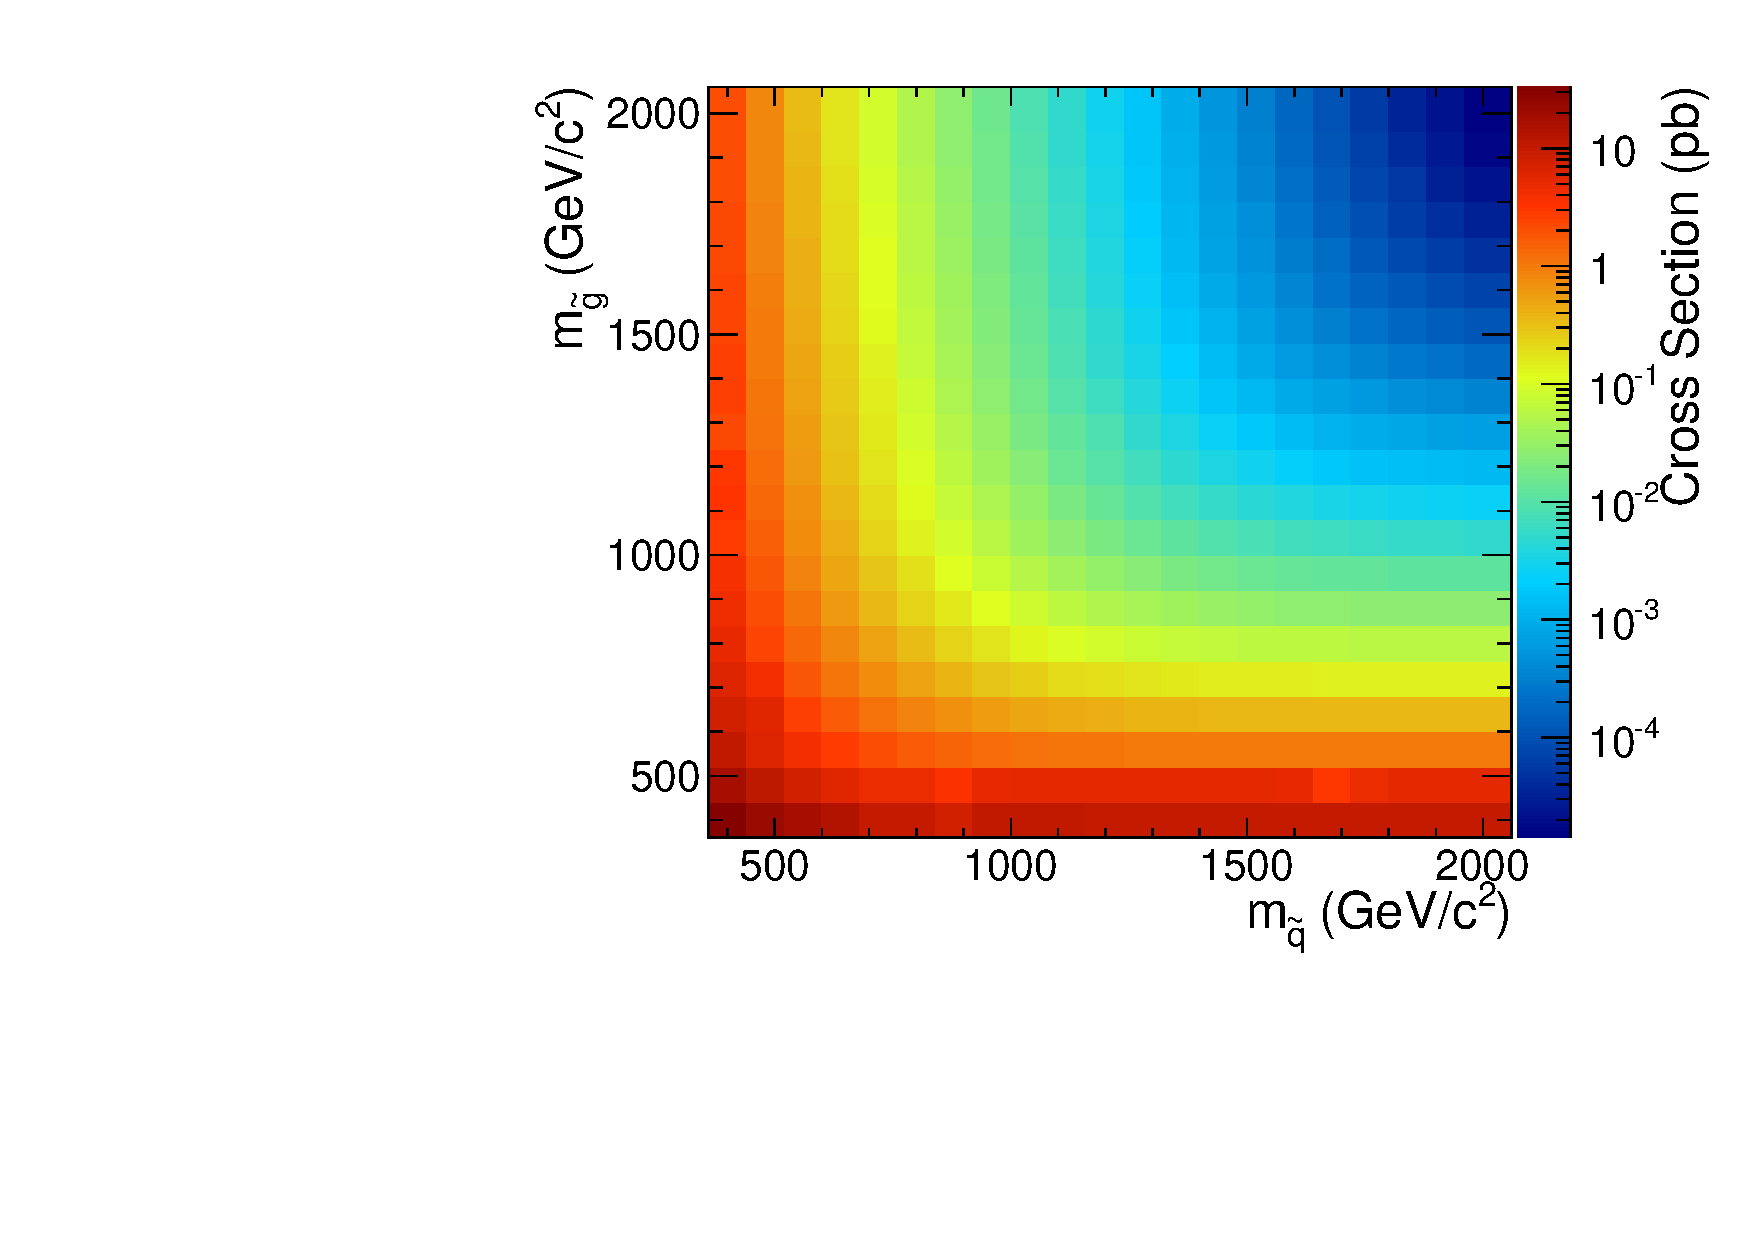
\includegraphics[scale=0.3]{can_xsec_bino_mN375_met100_nojet}}
	\\
	\subfloat[$M_{1}$ decoupled ($M_{1}$ = 3.5 TeV), $M_{2}$ = 375 GeV, $M_{3}$ vs. $m_{\tilde{q}}$.]{\label{fig:sig_xsec_mgluino_vs_msquark_wino}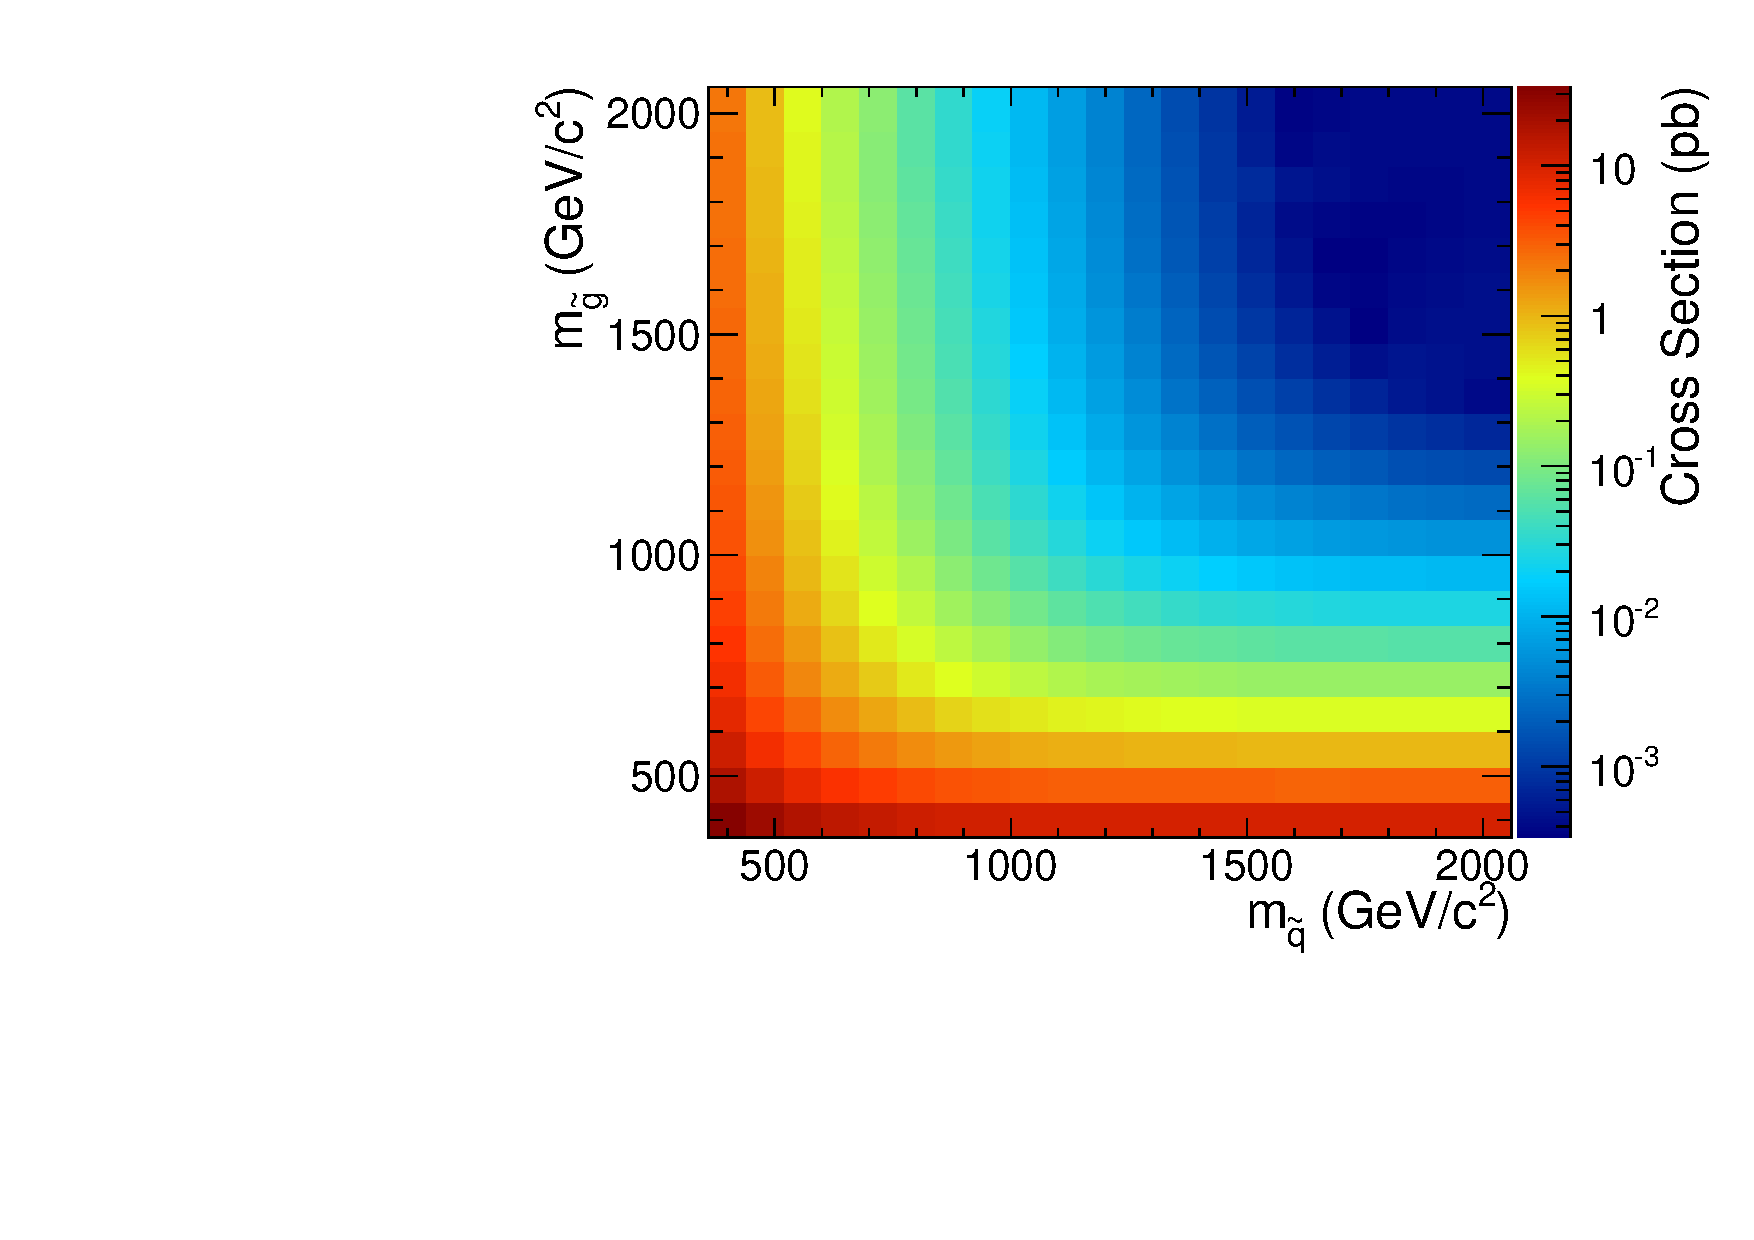
\includegraphics[scale=0.3]{can_xsec_wino_mN375_met100_nojet}}
	\\
	\subfloat[$m_{\tilde{q}}$ decoupled ($m_{\tilde{q}}$ = 2.5 TeV), $M_{3}$ vs. $M_{1}$.]{\label{fig:sig_xsec_mgluino_vs_mbino_old}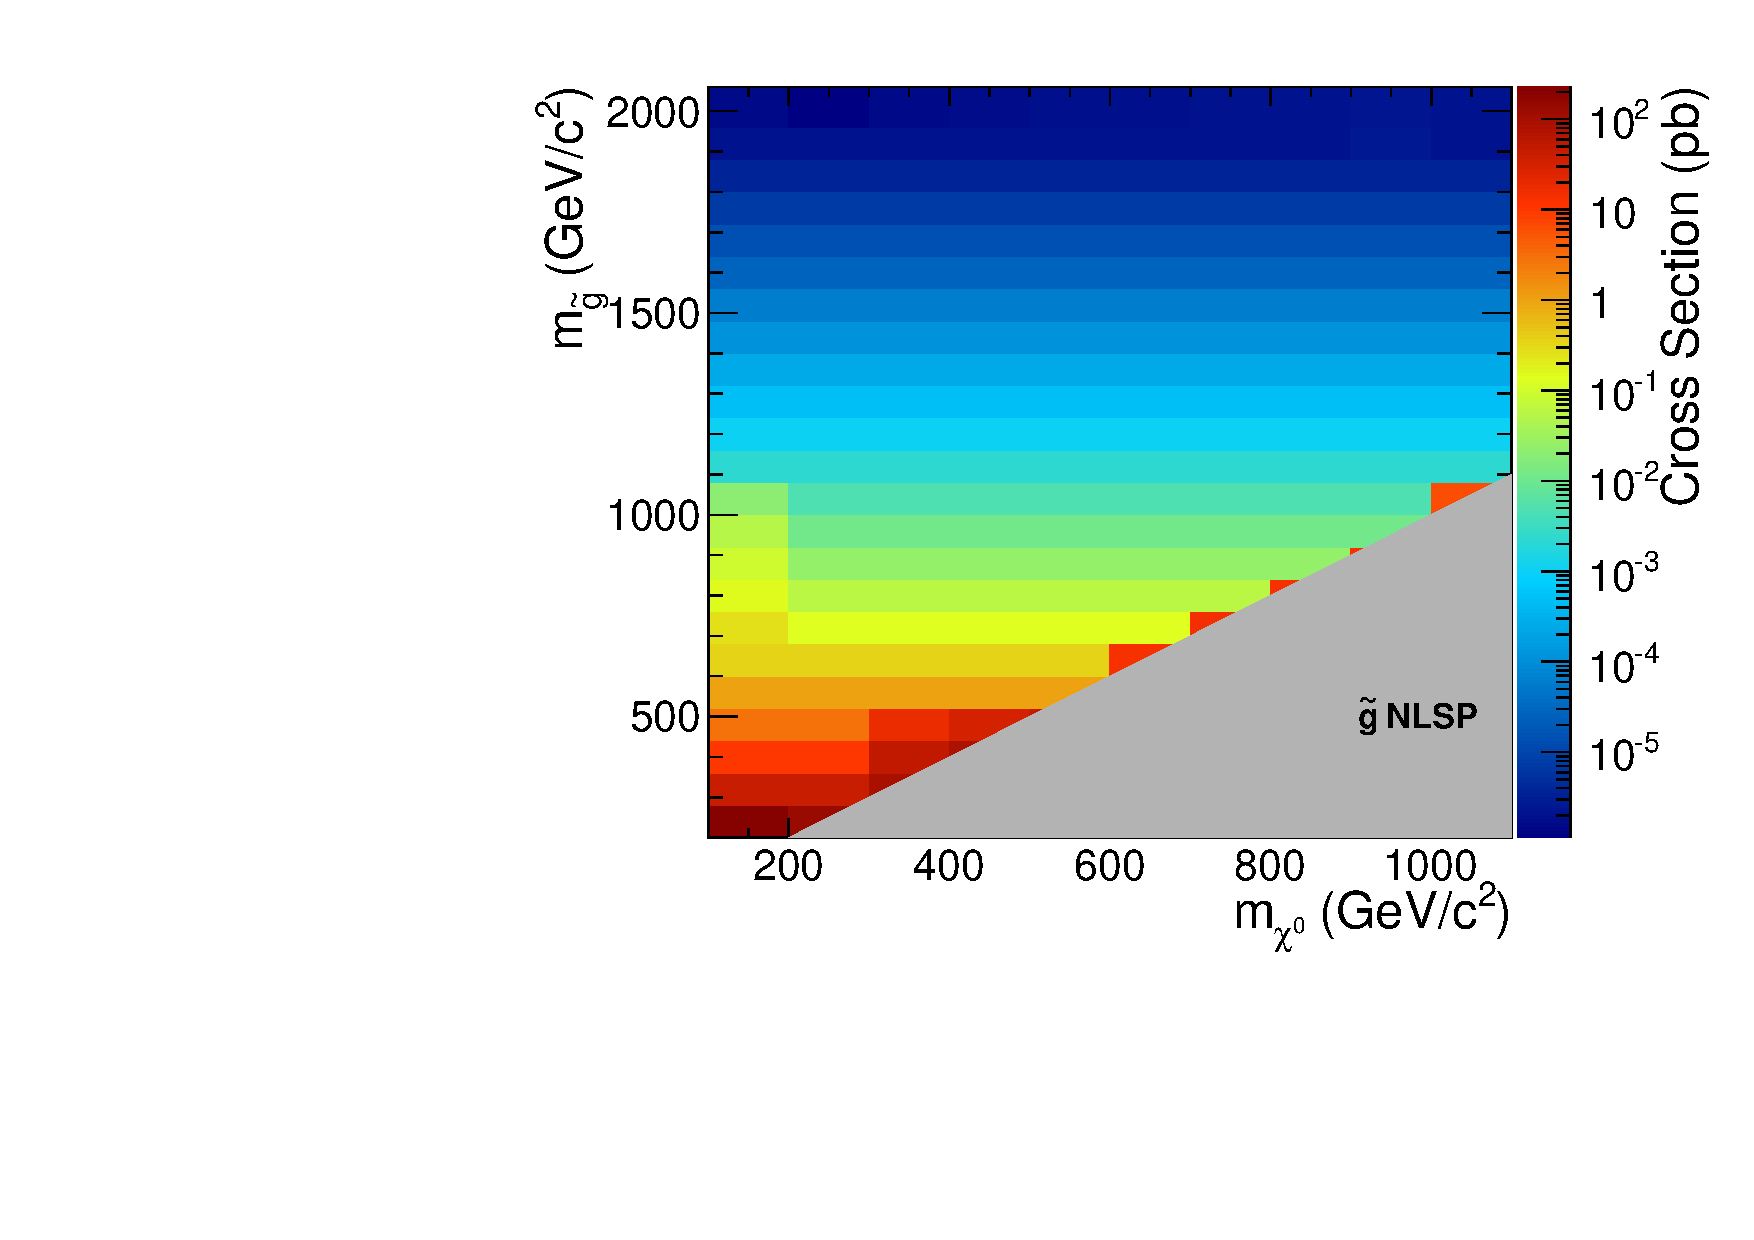
\includegraphics[scale=0.3]{can_xsec_bino_mNScan_met100_nojet}}
	\caption{Next to leading order cross sections for the three different MC scenarios described in the text.}
	\label{fig:sig_xsec}
\end{figure}

\section{Upper Limit Calculation and Model Exclusion}
\label{sec:Upper Limit Calculation and Model Exclusion}

The upper limits are calculated according to the prescription followed for the 2011 ATLAS + CMS Higgs limit combination \cite{CMS-NOTE-2011/005}.  This prescription utilizes the frequentist $\mbox{CL}_{s}$ method \cite{Read} with profile likelihood test statistic \cite{Cowan_Cranmer_Gross_Vitells}.  The $\mbox{CL}_{s}$ method and the profile likelihood are explained in Section~\ref{sec:CLs and the Profile Likelihood Test Statistic}, using specific signal MC points to illustrate the procedure.  First, however, the signal MC acceptance $\times$ efficiency, which is an input to the limit setting procedure, is presented in Section~\ref{sec:Signal Acceptance Times Efficiency}.

\subsection{Signal Acceptance $\times$ Efficiency}
\label{sec:Signal Acceptance Times Efficiency}

The signal acceptance $\times$ efficiency (denoted $\mathcal{A}\times\epsilon$), defined for each signal point as the number of $\gamma\gamma$ events selected with \MET $\geq$ 50 GeV divided by the total number of events generated, is shown in Figure~\ref{fig:sig_Axe} for the three different scenarios described in Sec.~\ref{sec:Simplified Models}.  Acceptance refers to the fraction of true events that can be detected given the fiducial extent of the detector and the $E_{T}$ cuts on the photons.  Efficiency denotes the fraction of accepted events (i.e. those events passing the $E_{T}$ and $\eta$ cuts) that have two photons passing the photon identification criteria.

\begin{figure}
	\centering
%	\subfloat[$M_{2}$ decoupled ($M_{2}$ = 2 TeV), $M_{1}$ = 375 GeV, $M_{3}$ vs. $m_{\tilde{q}}$.]{\label{fig:sig_Axe_mgluino_vs_msquark}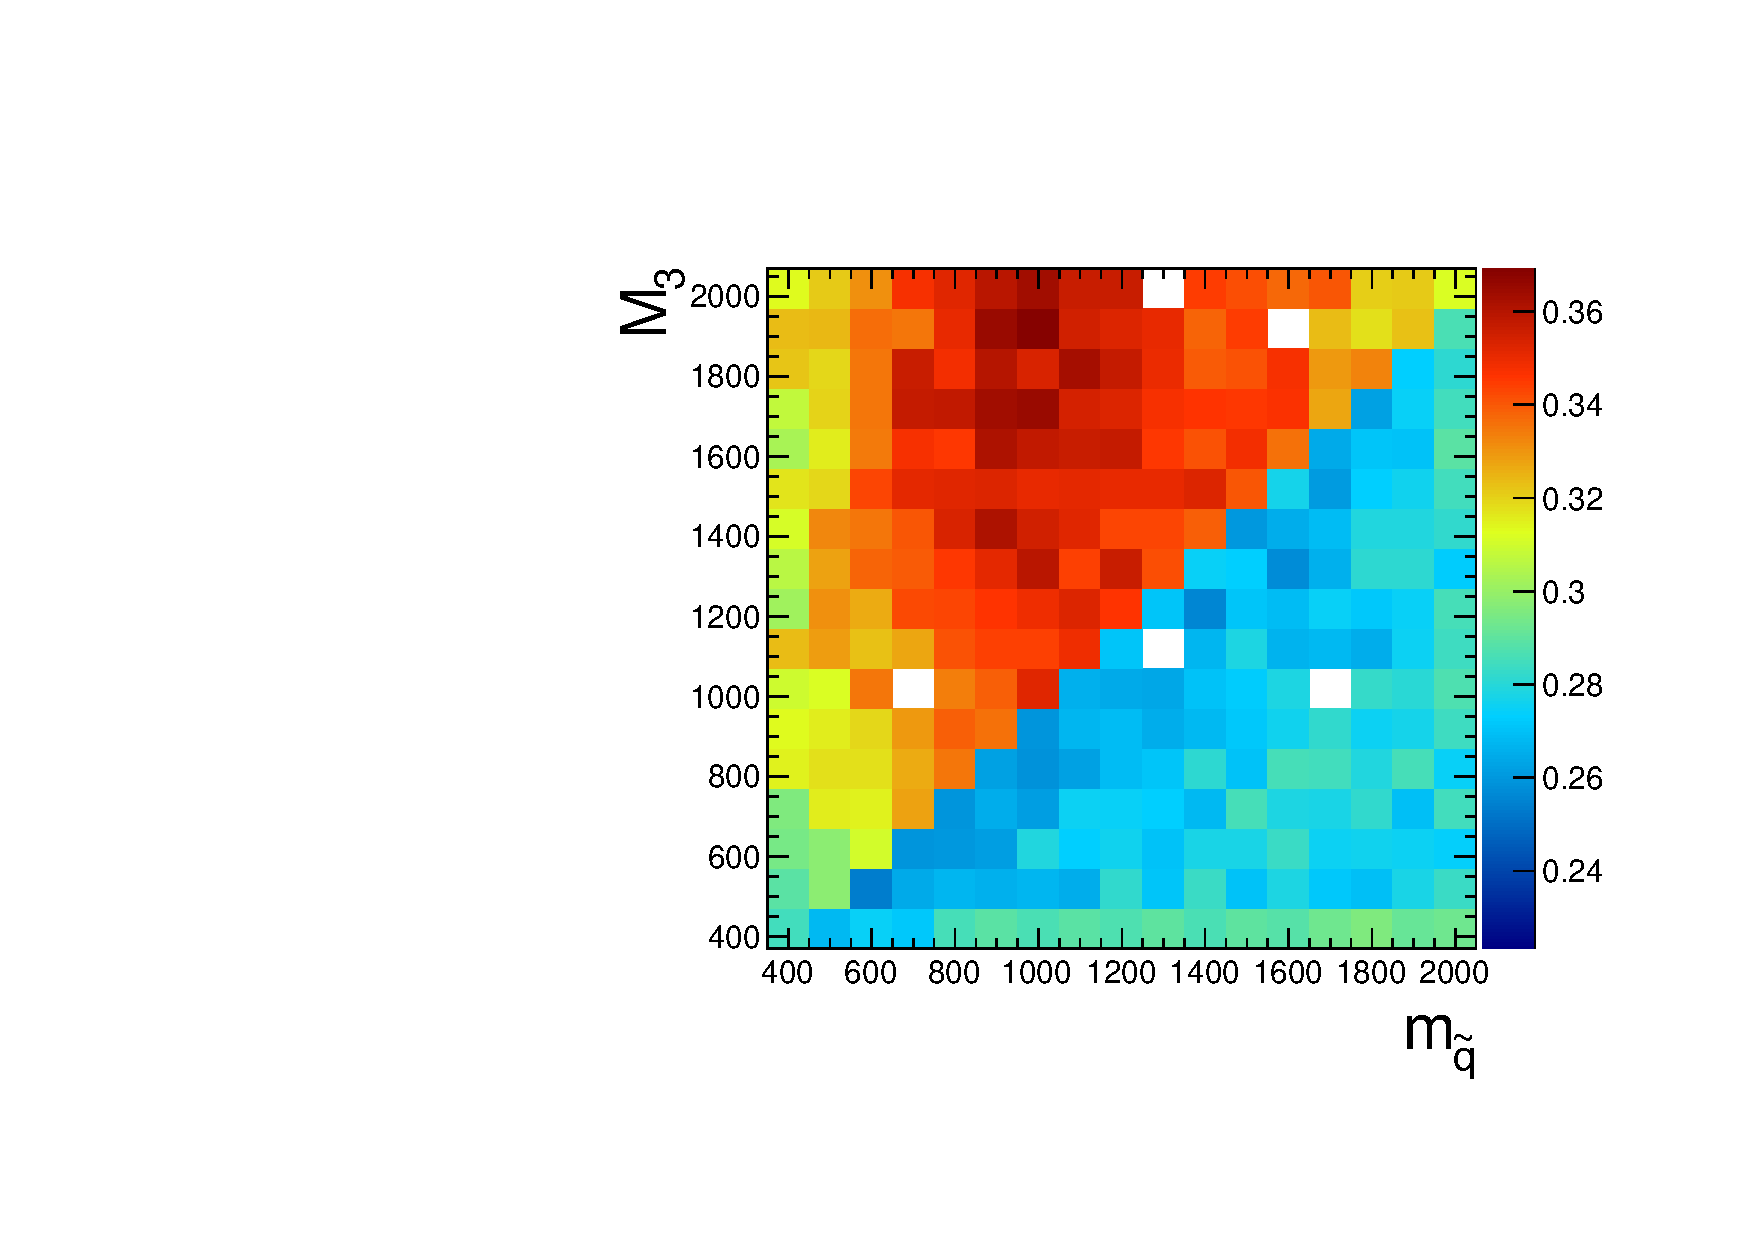
\includegraphics[scale=0.3]{mgluino_vs_msquark_METGeq50GeV}}
%	\\
%	\subfloat[$m_{\tilde{q}}$ decoupled ($m_{\tilde{q}}$ = 5 TeV), $M_{3}$ vs. $M_{1}$.]{\label{fig:sig_Axe_mgluino_vs_mbino}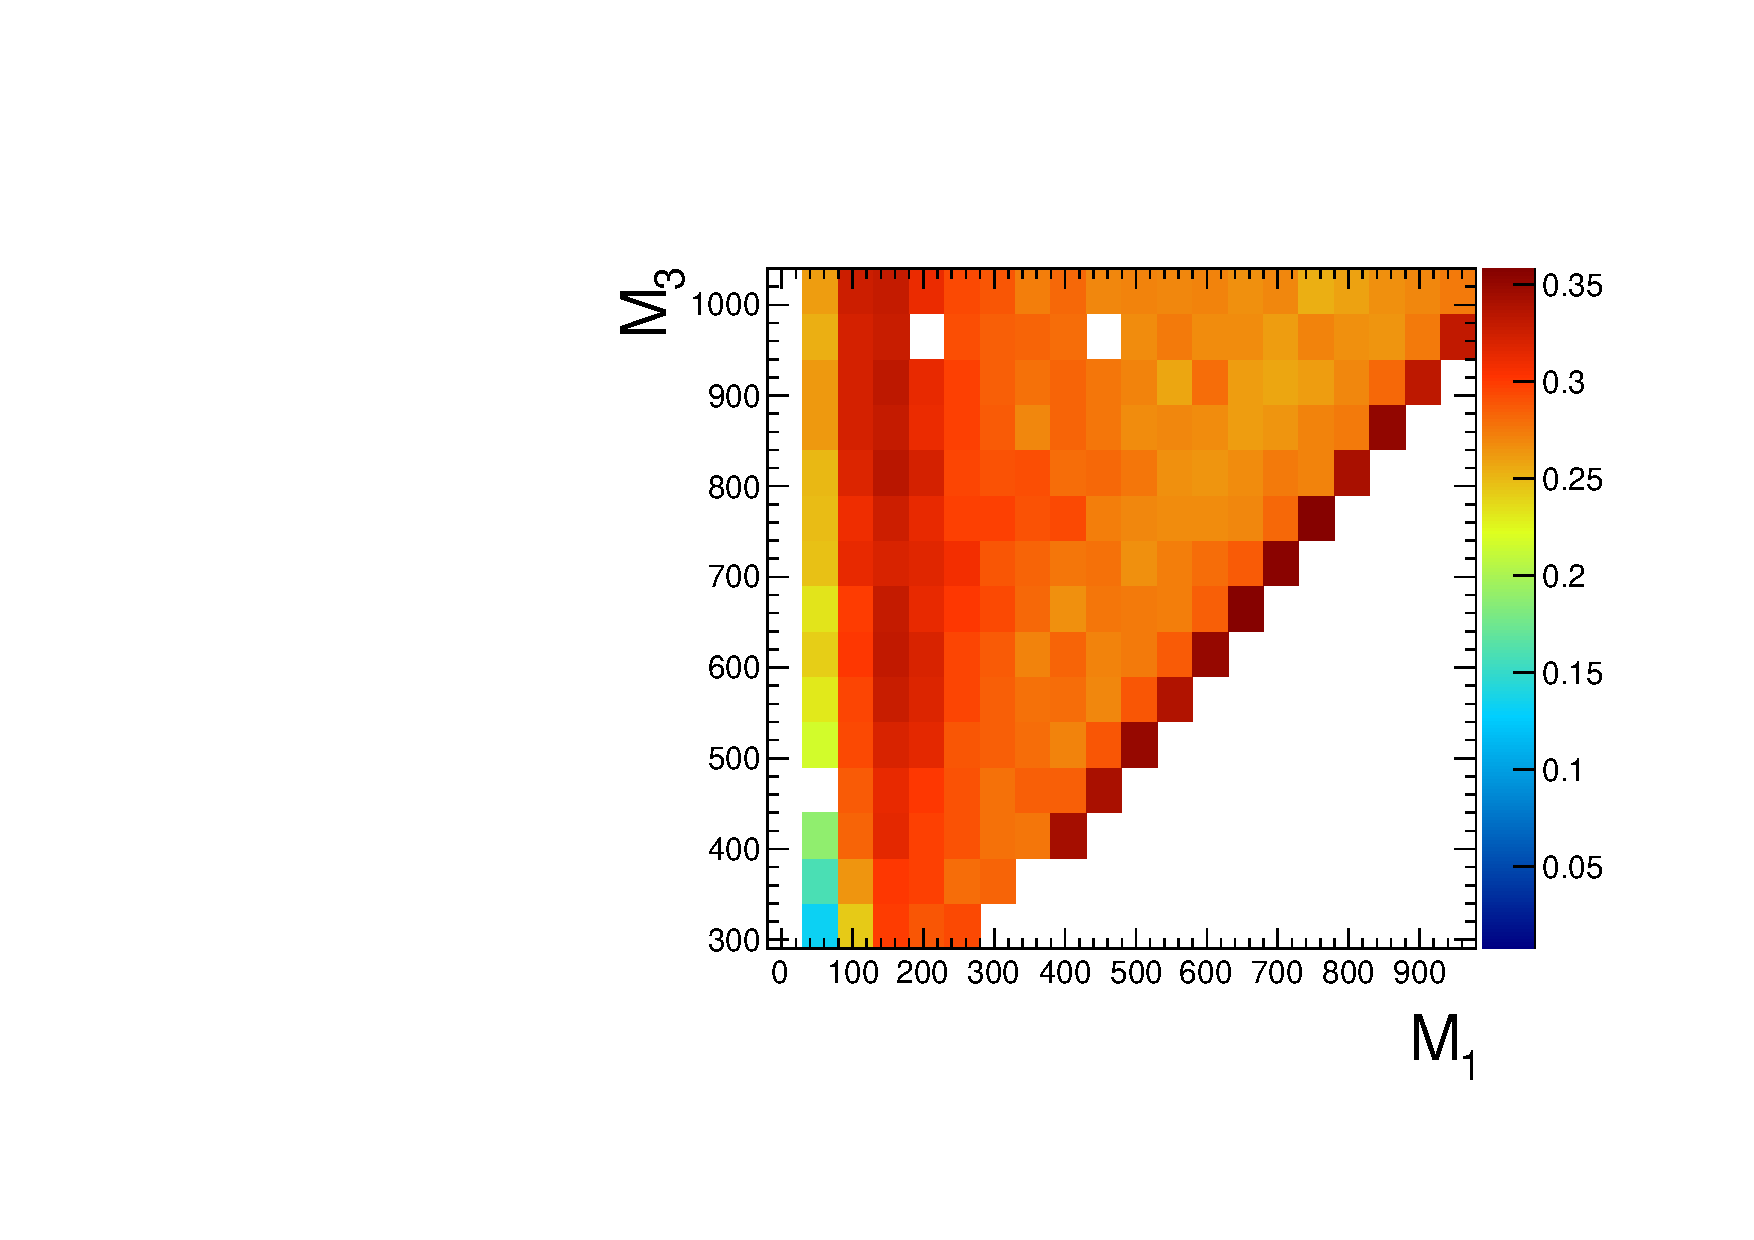
\includegraphics[scale=0.3]{mgluino_vs_mbino_METGeq50GeV}}
%	\\
%	\subfloat[$M_{3}$ and $m_{\tilde{q}}$ decoupled ($M_{3} = m_{\tilde{q}}$ = 5 TeV), $M_{1}$ vs. $M_{2}$.]{\label{fig:sig_Axe_mbino_vs_mwino}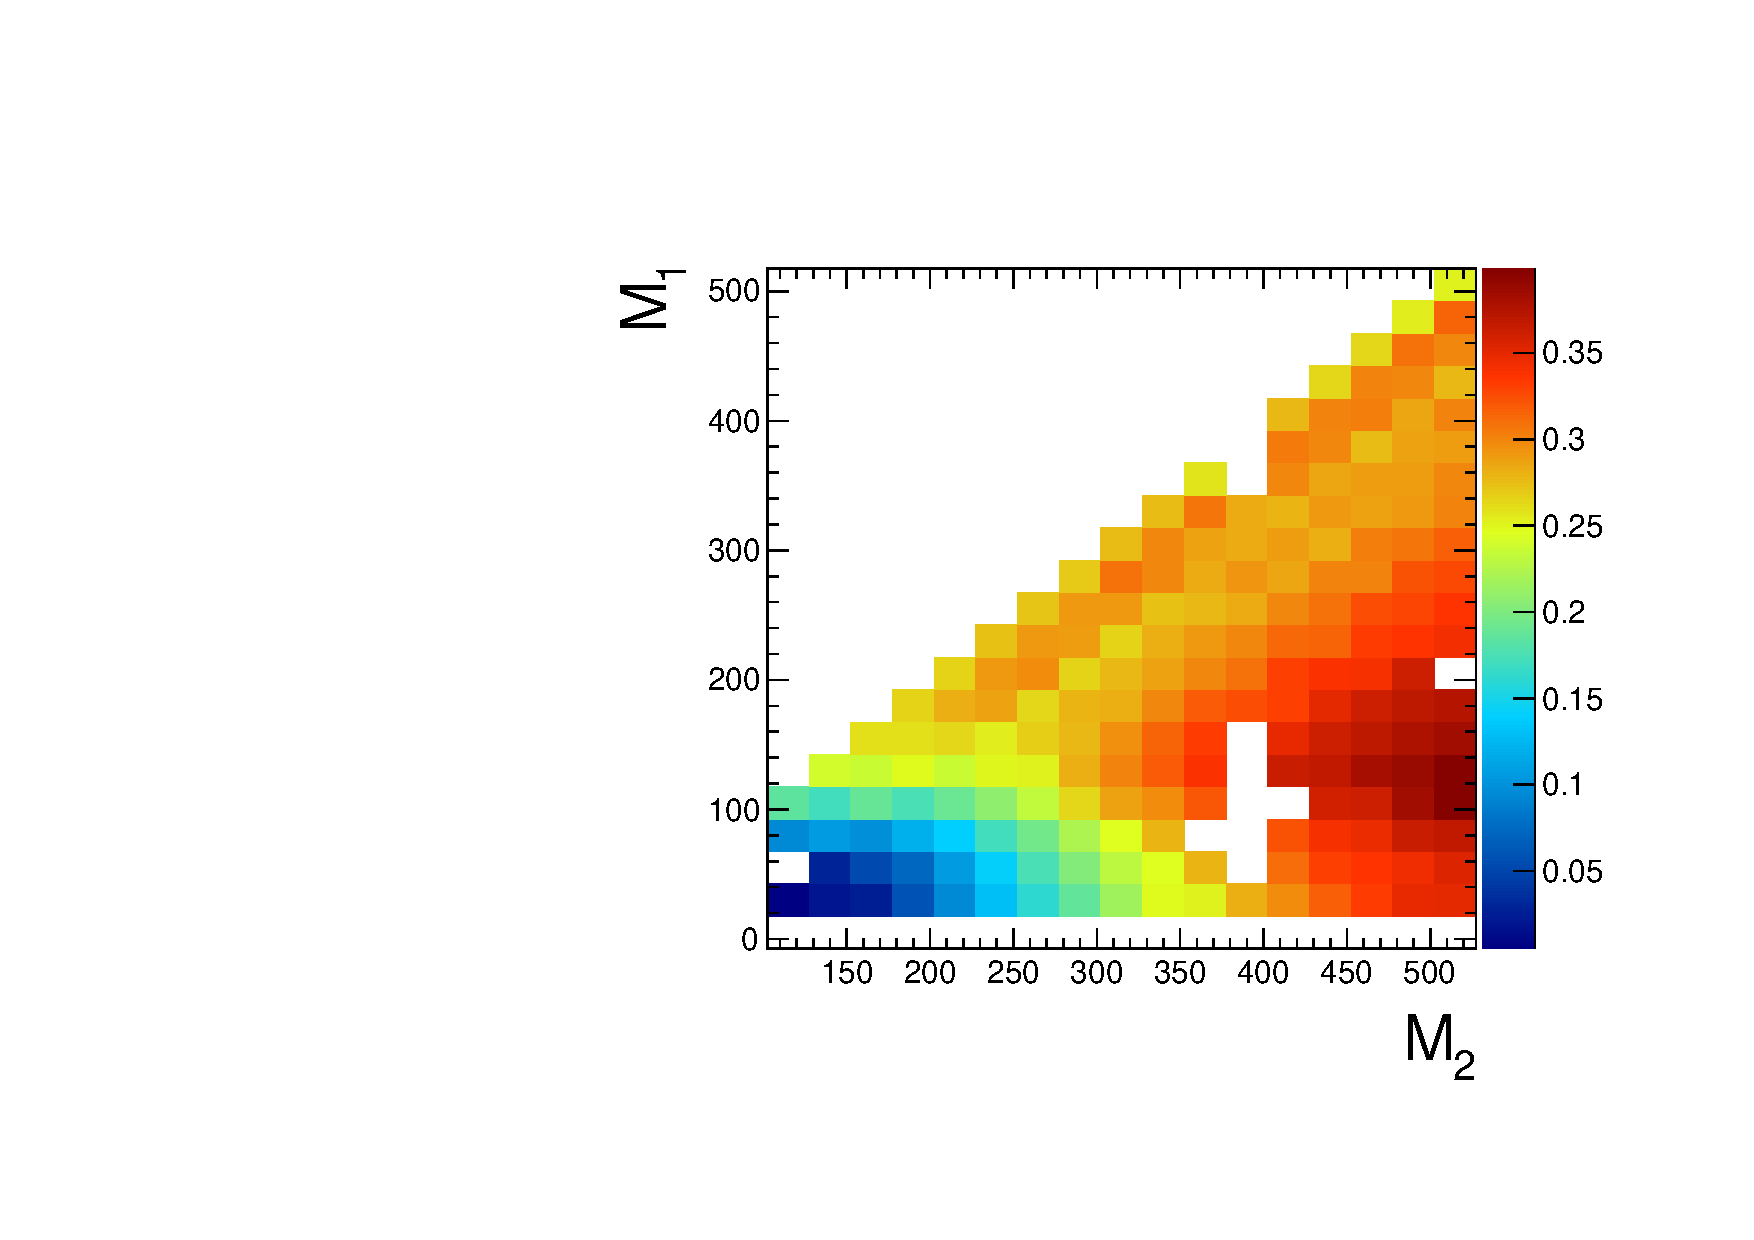
\includegraphics[scale=0.3]{mbino_vs_mwino_METGeq50GeV}}
%	\\
	\subfloat[$M_{2}$ decoupled ($M_{2}$ = 3.5 TeV), $M_{1}$ = 375 GeV, $M_{3}$ vs. $m_{\tilde{q}}$, $\geq0$ jets.]{\label{fig:sig_Axe_mgluino_vs_msquark_bino}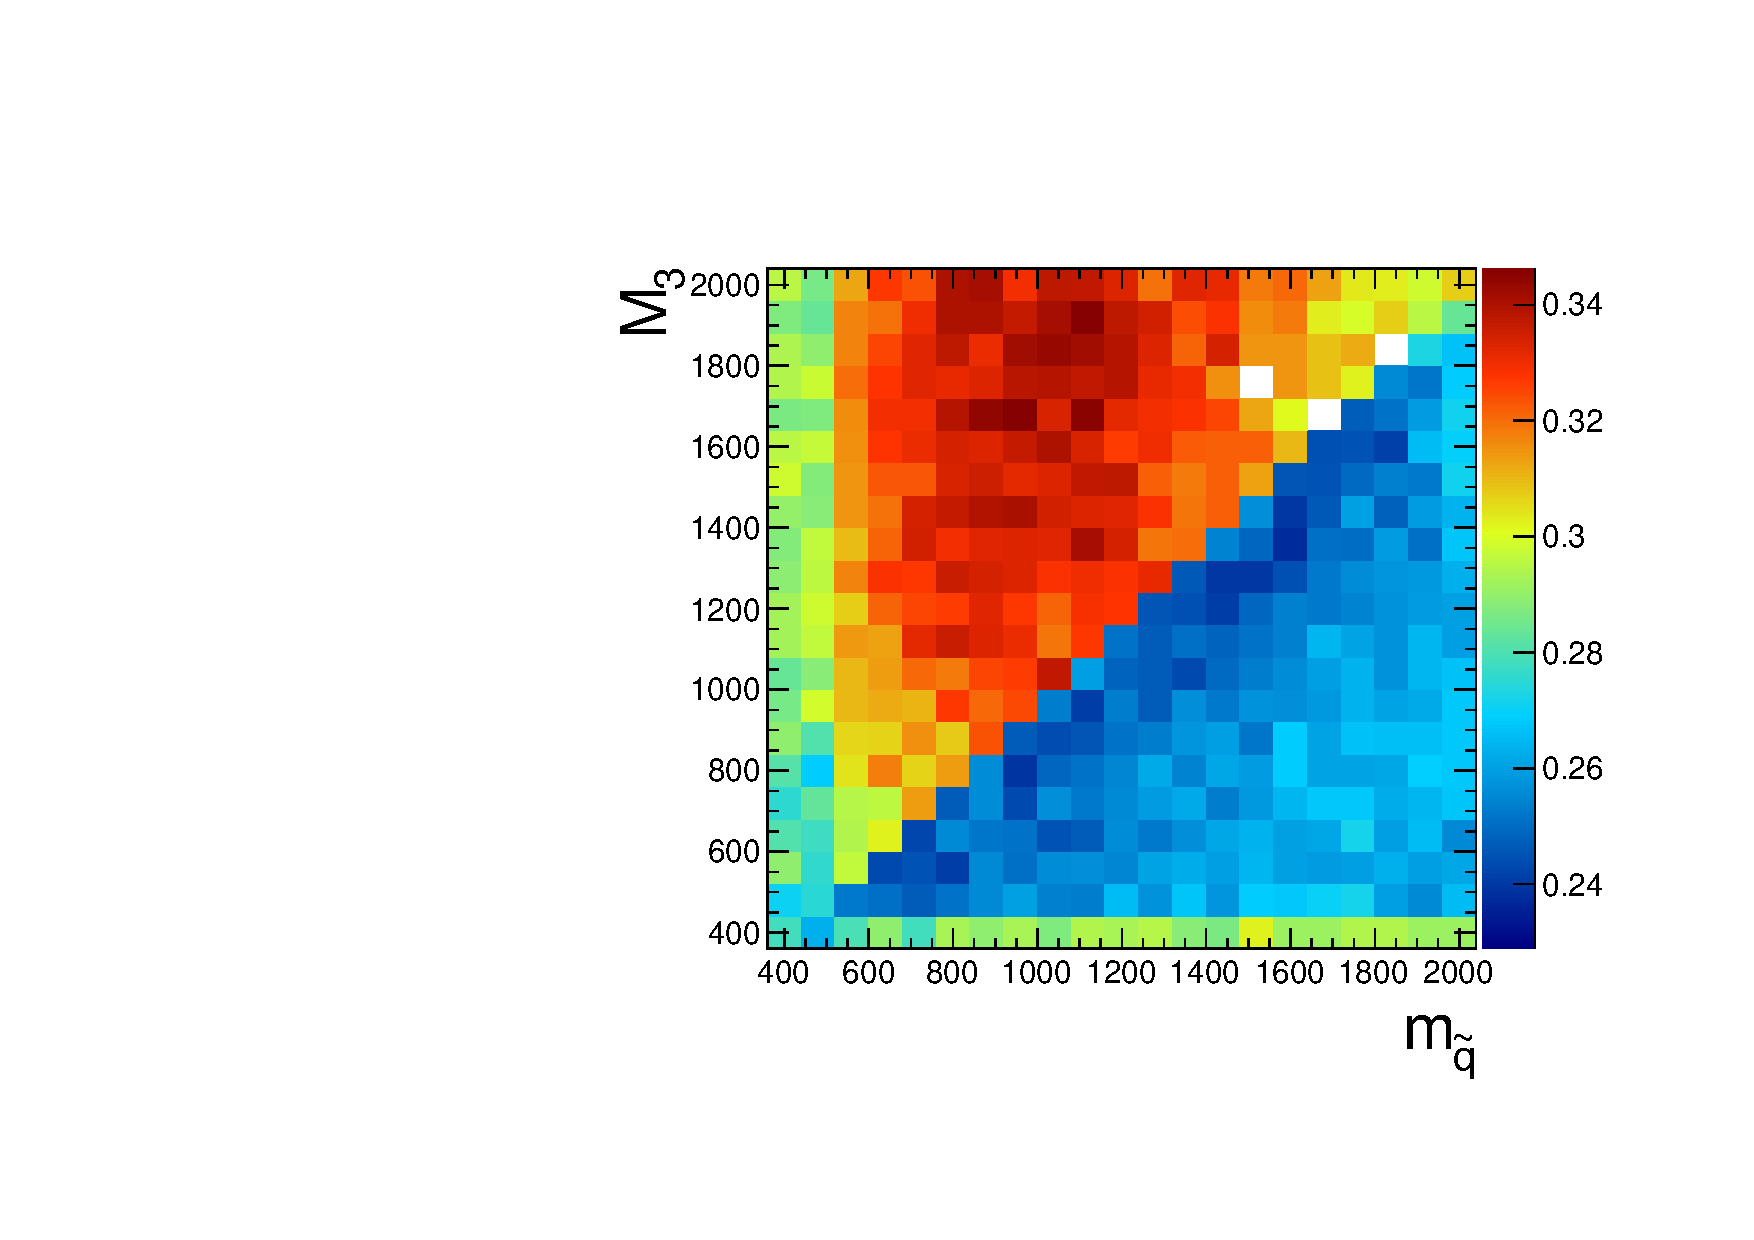
\includegraphics[scale=0.3]{mgluino_vs_msquark_METGeq50GeV_bino_old}}
	\hspace{1cm}
	\subfloat[$M_{2}$ decoupled ($M_{2}$ = 3.5 TeV), $M_{1}$ = 375 GeV, $M_{3}$ vs. $m_{\tilde{q}}$, $\geq1$ jet.]{\label{fig:sig_Axe_mgluino_vs_msquark_bino_1jet}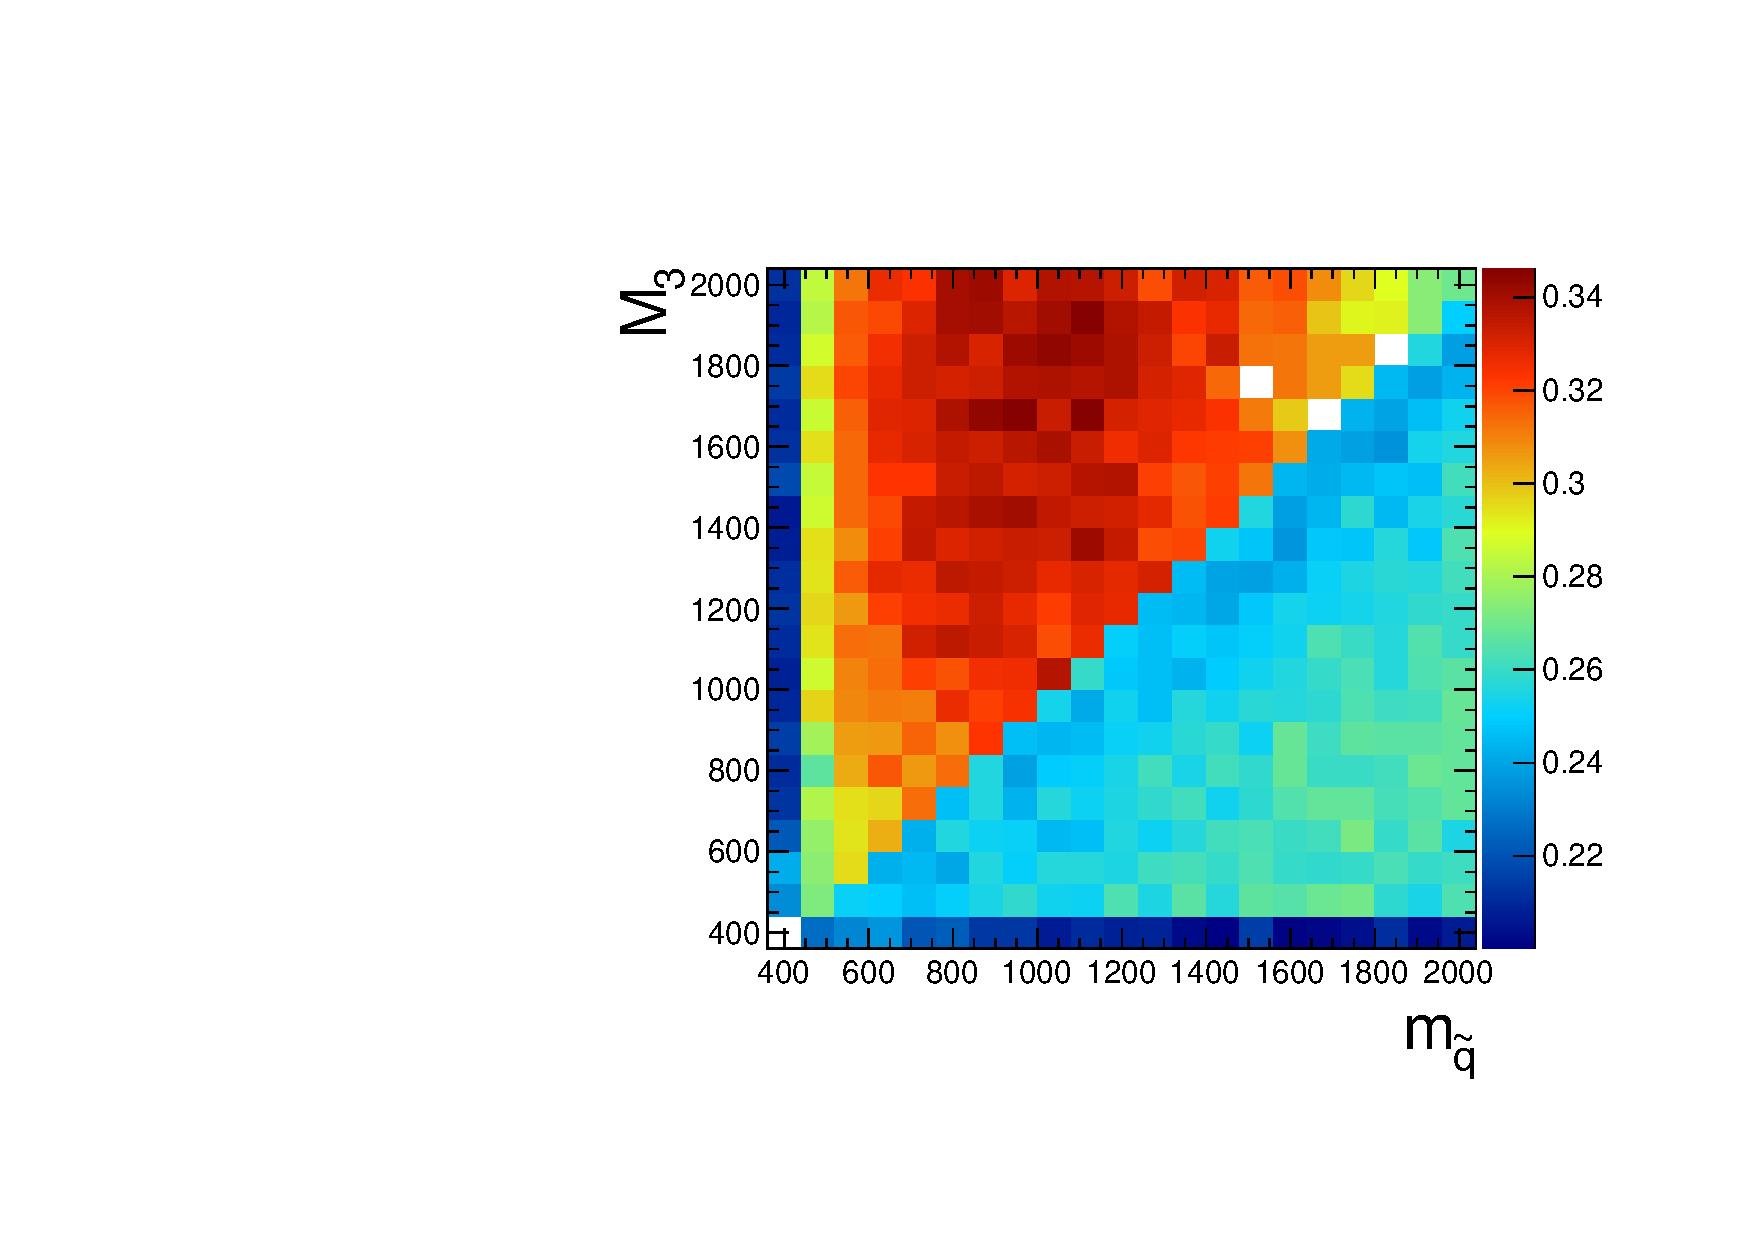
\includegraphics[scale=0.3]{mgluino_vs_msquark_METGeq50GeV_bino_old_1jet}}
	\\
	\subfloat[$M_{1}$ decoupled ($M_{1}$ = 3.5 TeV), $M_{2}$ = 375 GeV, $M_{3}$ vs. $m_{\tilde{q}}$, $\geq0$ jets.]{\label{fig:sig_Axe_mgluino_vs_msquark_wino}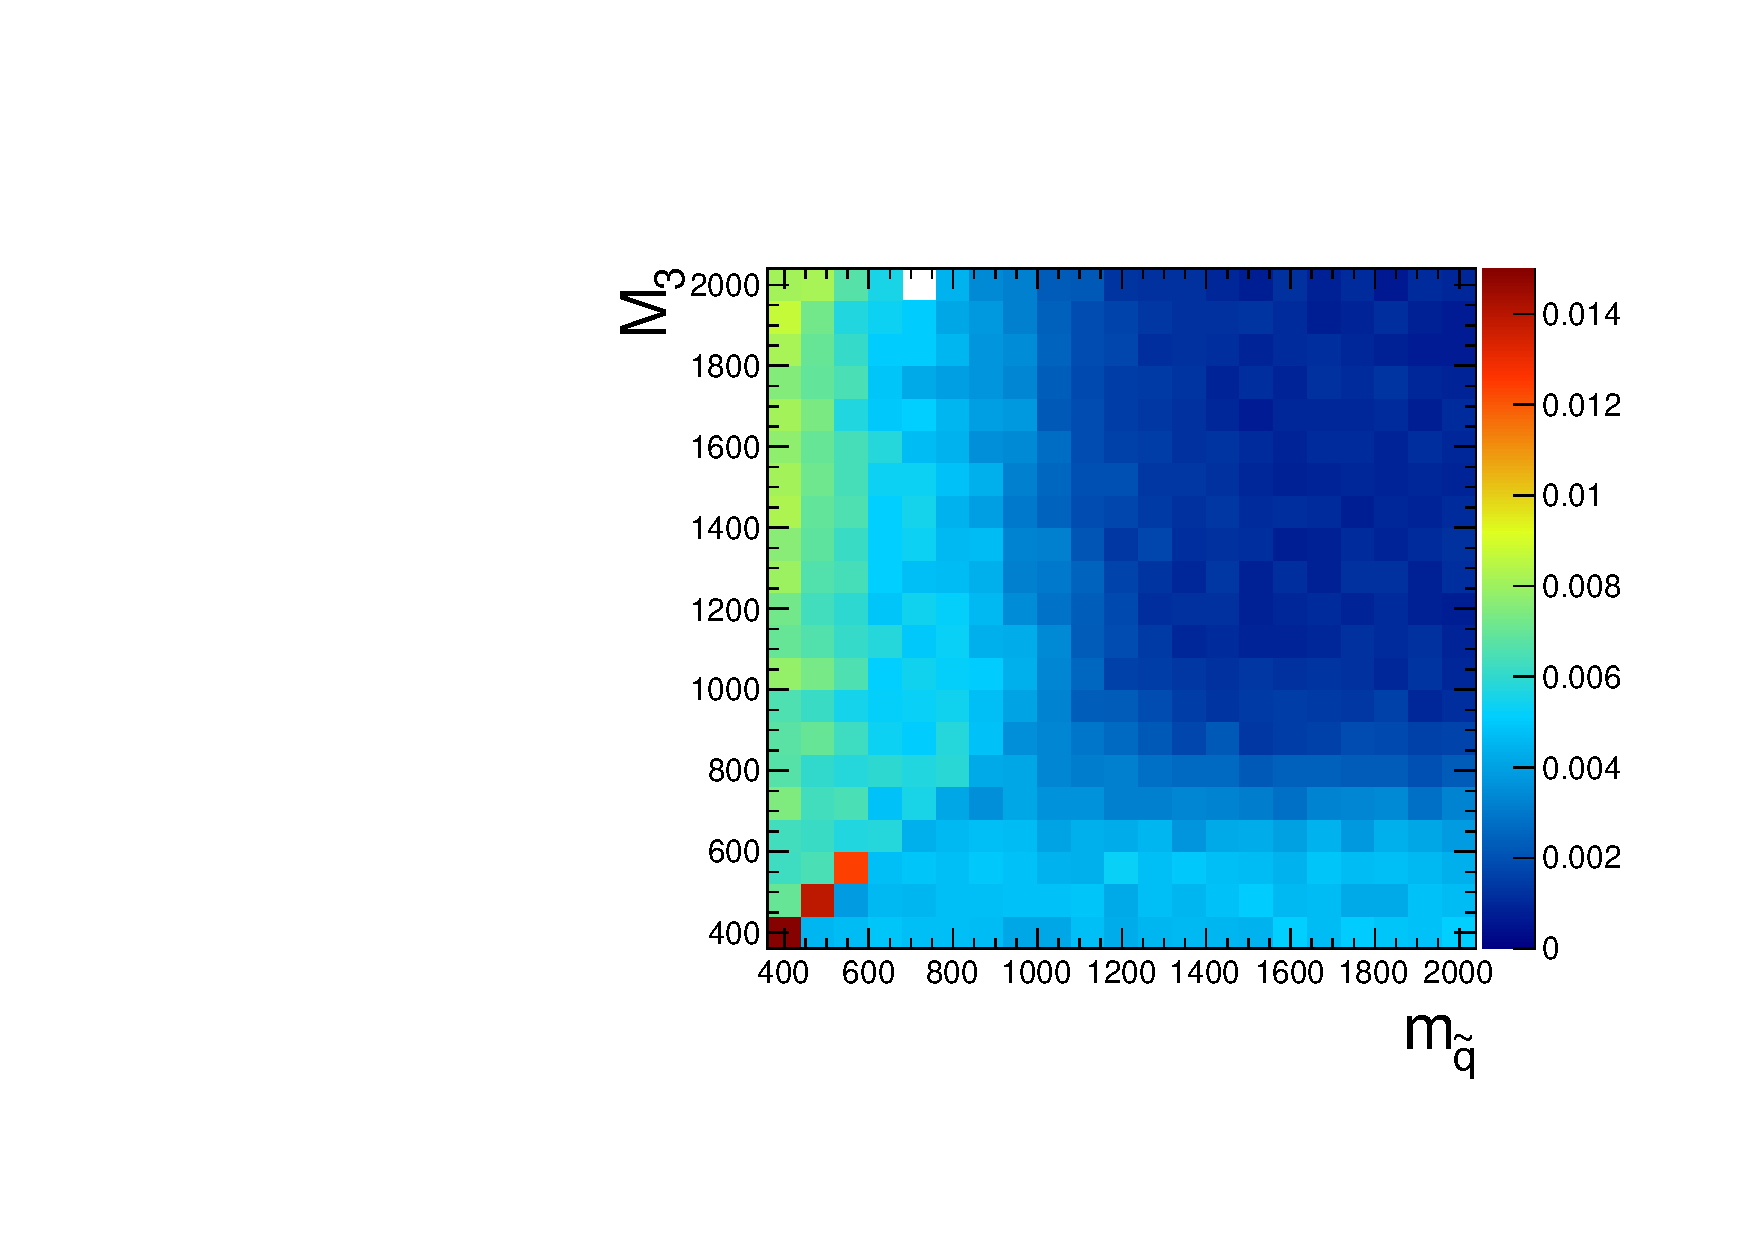
\includegraphics[scale=0.3]{mgluino_vs_msquark_METGeq50GeV_wino_old}}
	\hspace{1cm}
	\subfloat[$M_{1}$ decoupled ($M_{1}$ = 3.5 TeV), $M_{2}$ = 375 GeV, $M_{3}$ vs. $m_{\tilde{q}}$, $\geq1$ jet.]{\label{fig:sig_Axe_mgluino_vs_msquark_wino_1jet}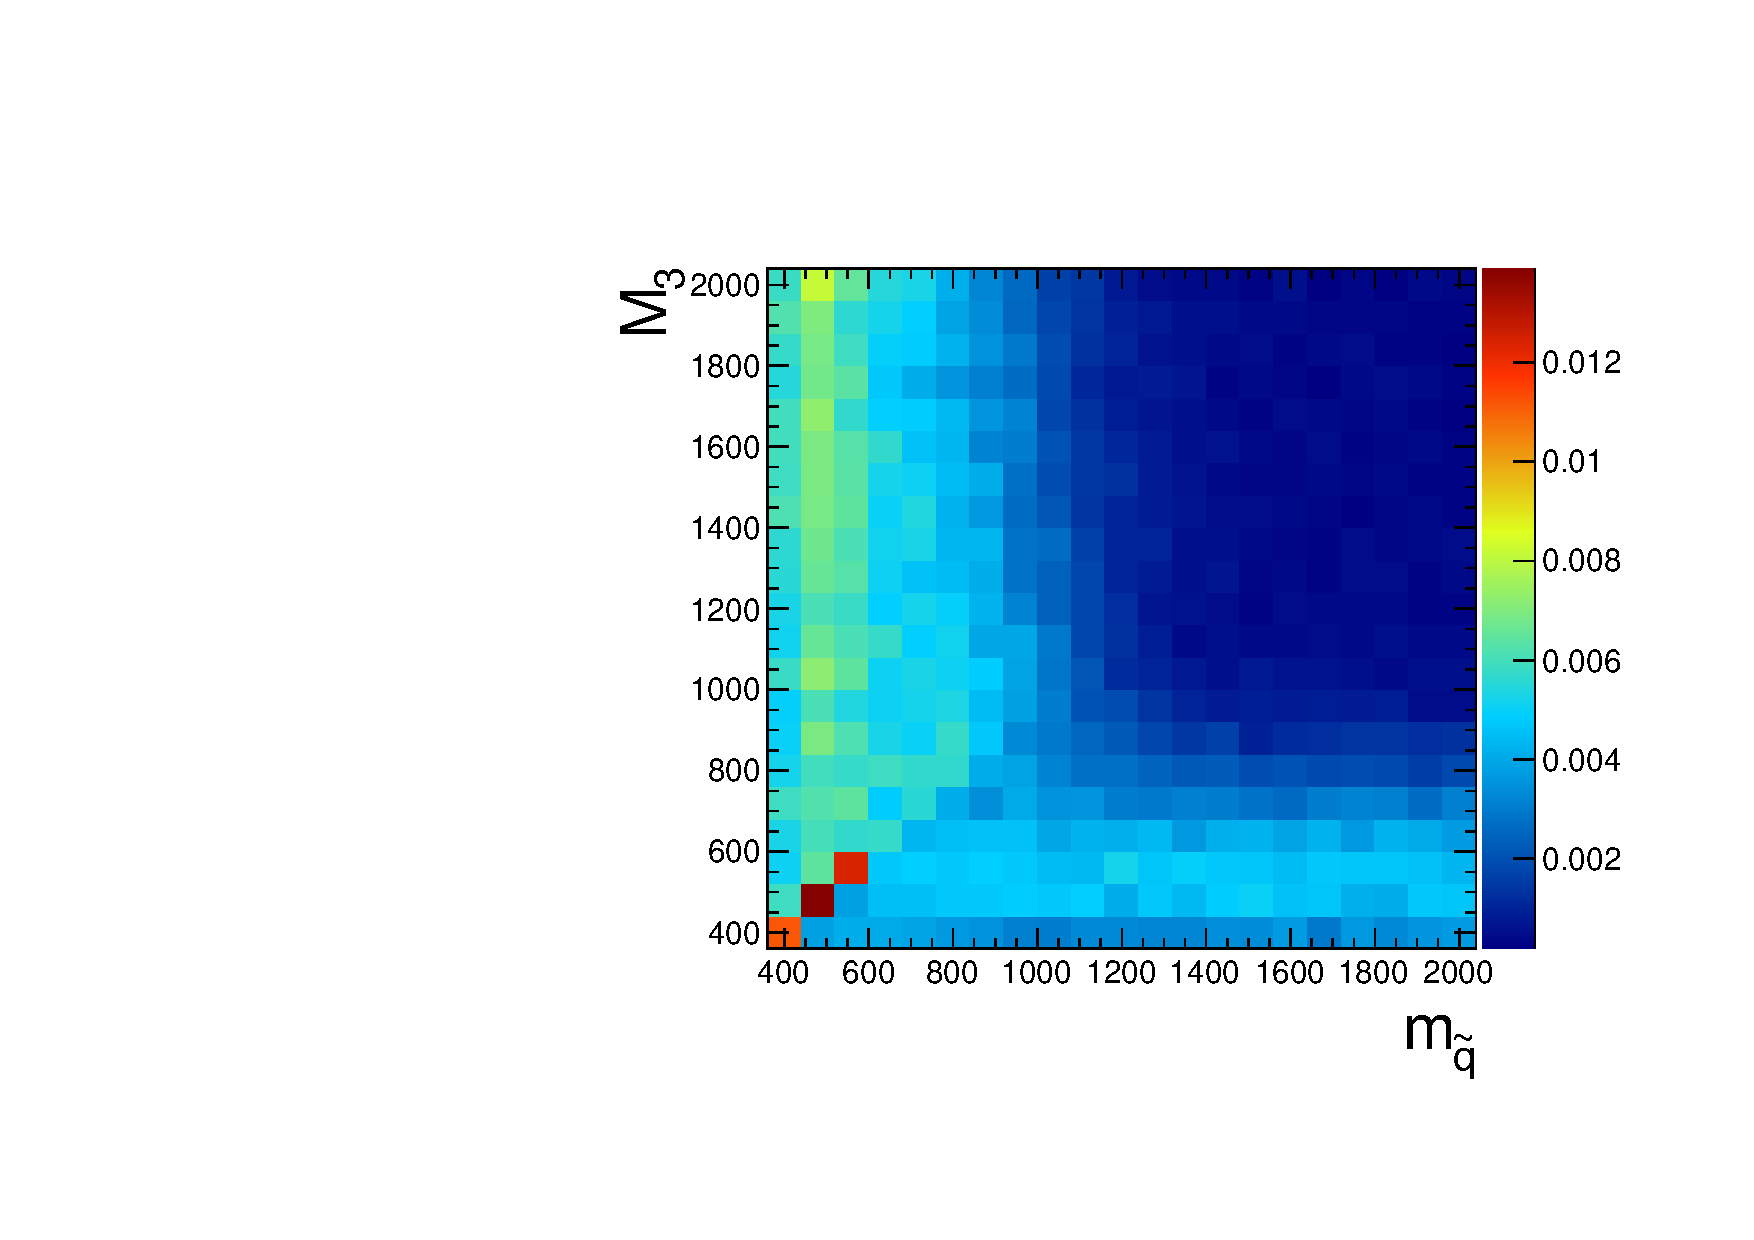
\includegraphics[scale=0.3]{mgluino_vs_msquark_METGeq50GeV_wino_old_1jet}}
	\\
	\subfloat[$m_{\tilde{q}}$ decoupled ($m_{\tilde{q}}$ = 2.5 TeV), $M_{3}$ vs. $M_{1}$, $\geq0$ jets.]{\label{fig:sig_Axe_mgluino_vs_mbino_old}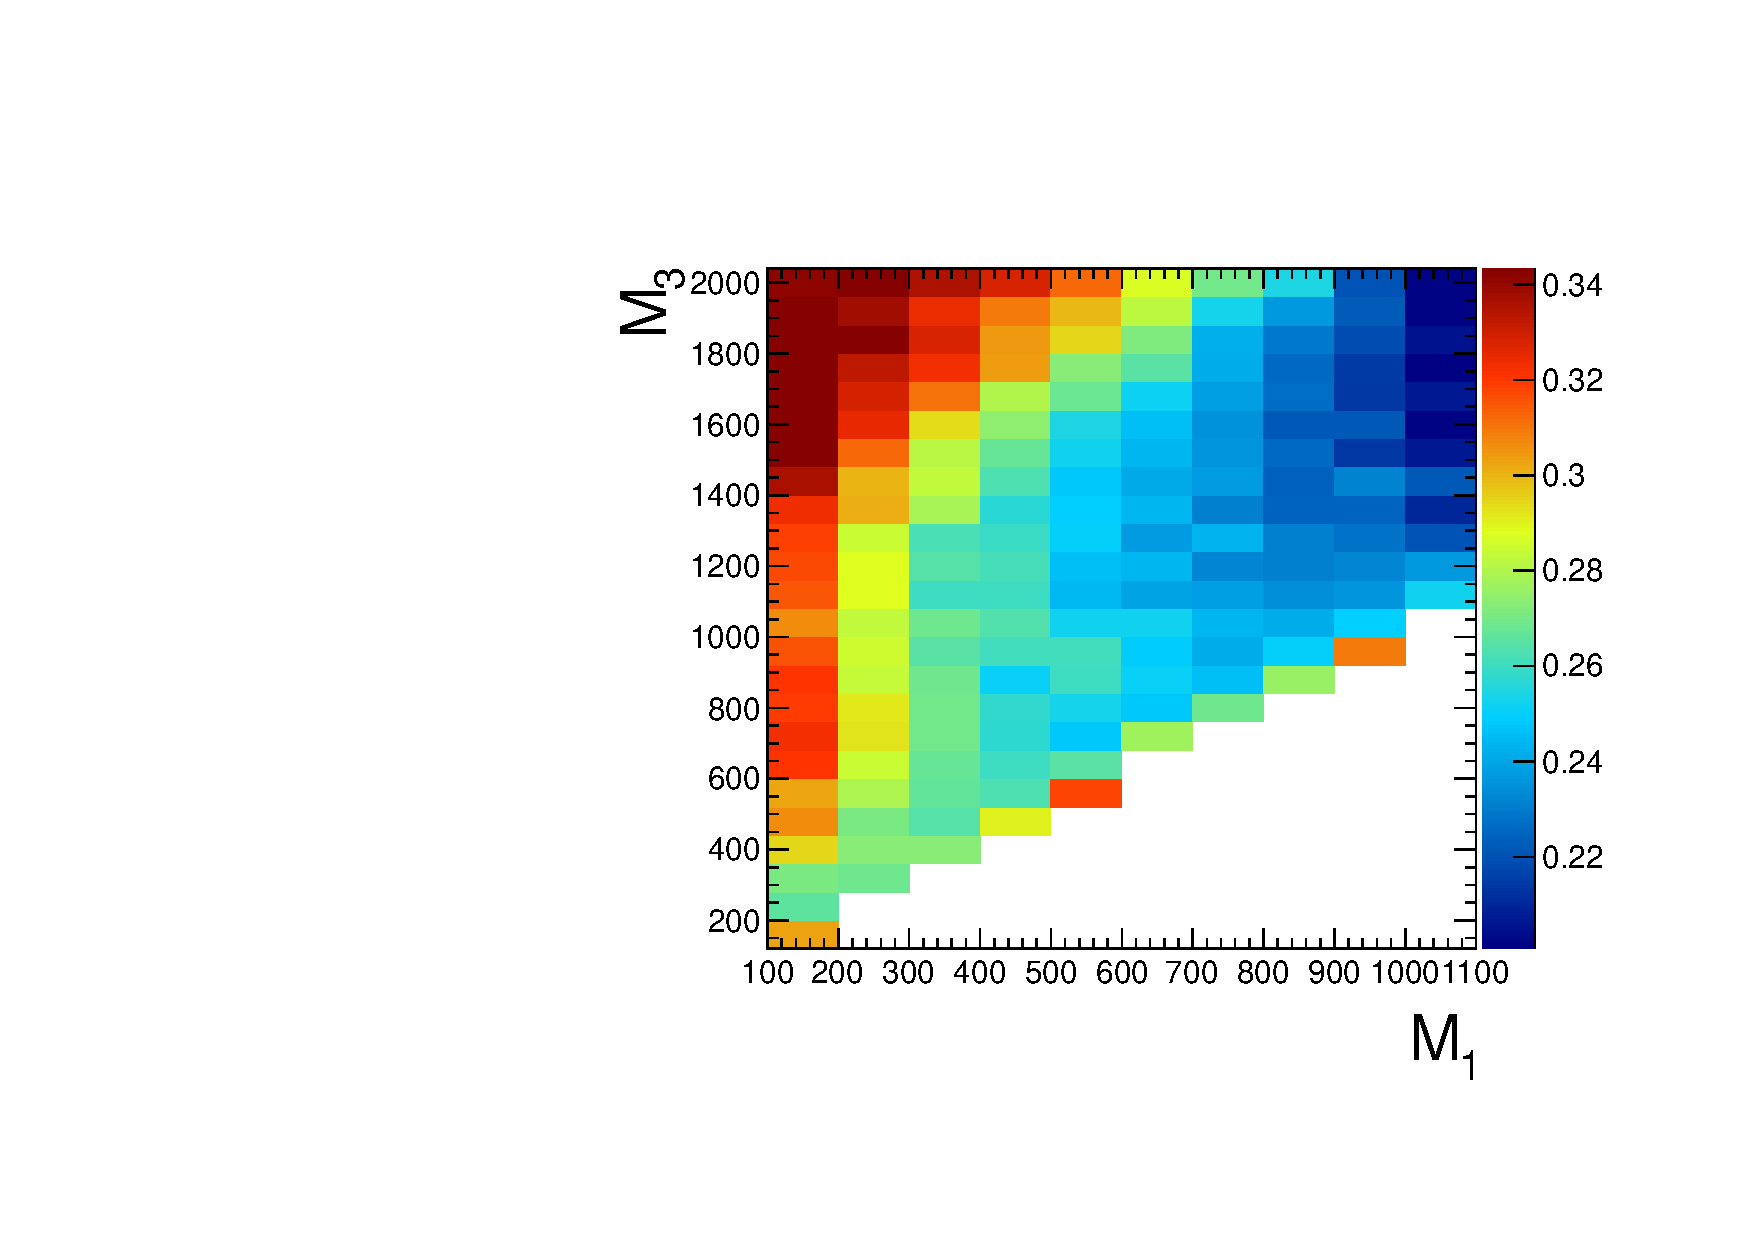
\includegraphics[scale=0.3]{mgluino_vs_mbino_METGeq50GeV_old}}
	\hspace{1cm}
	\subfloat[$m_{\tilde{q}}$ decoupled ($m_{\tilde{q}}$ = 2.5 TeV), $M_{3}$ vs. $M_{1}$, $\geq1$ jet.]{\label{fig:sig_Axe_mgluino_vs_mbino_old_1jet}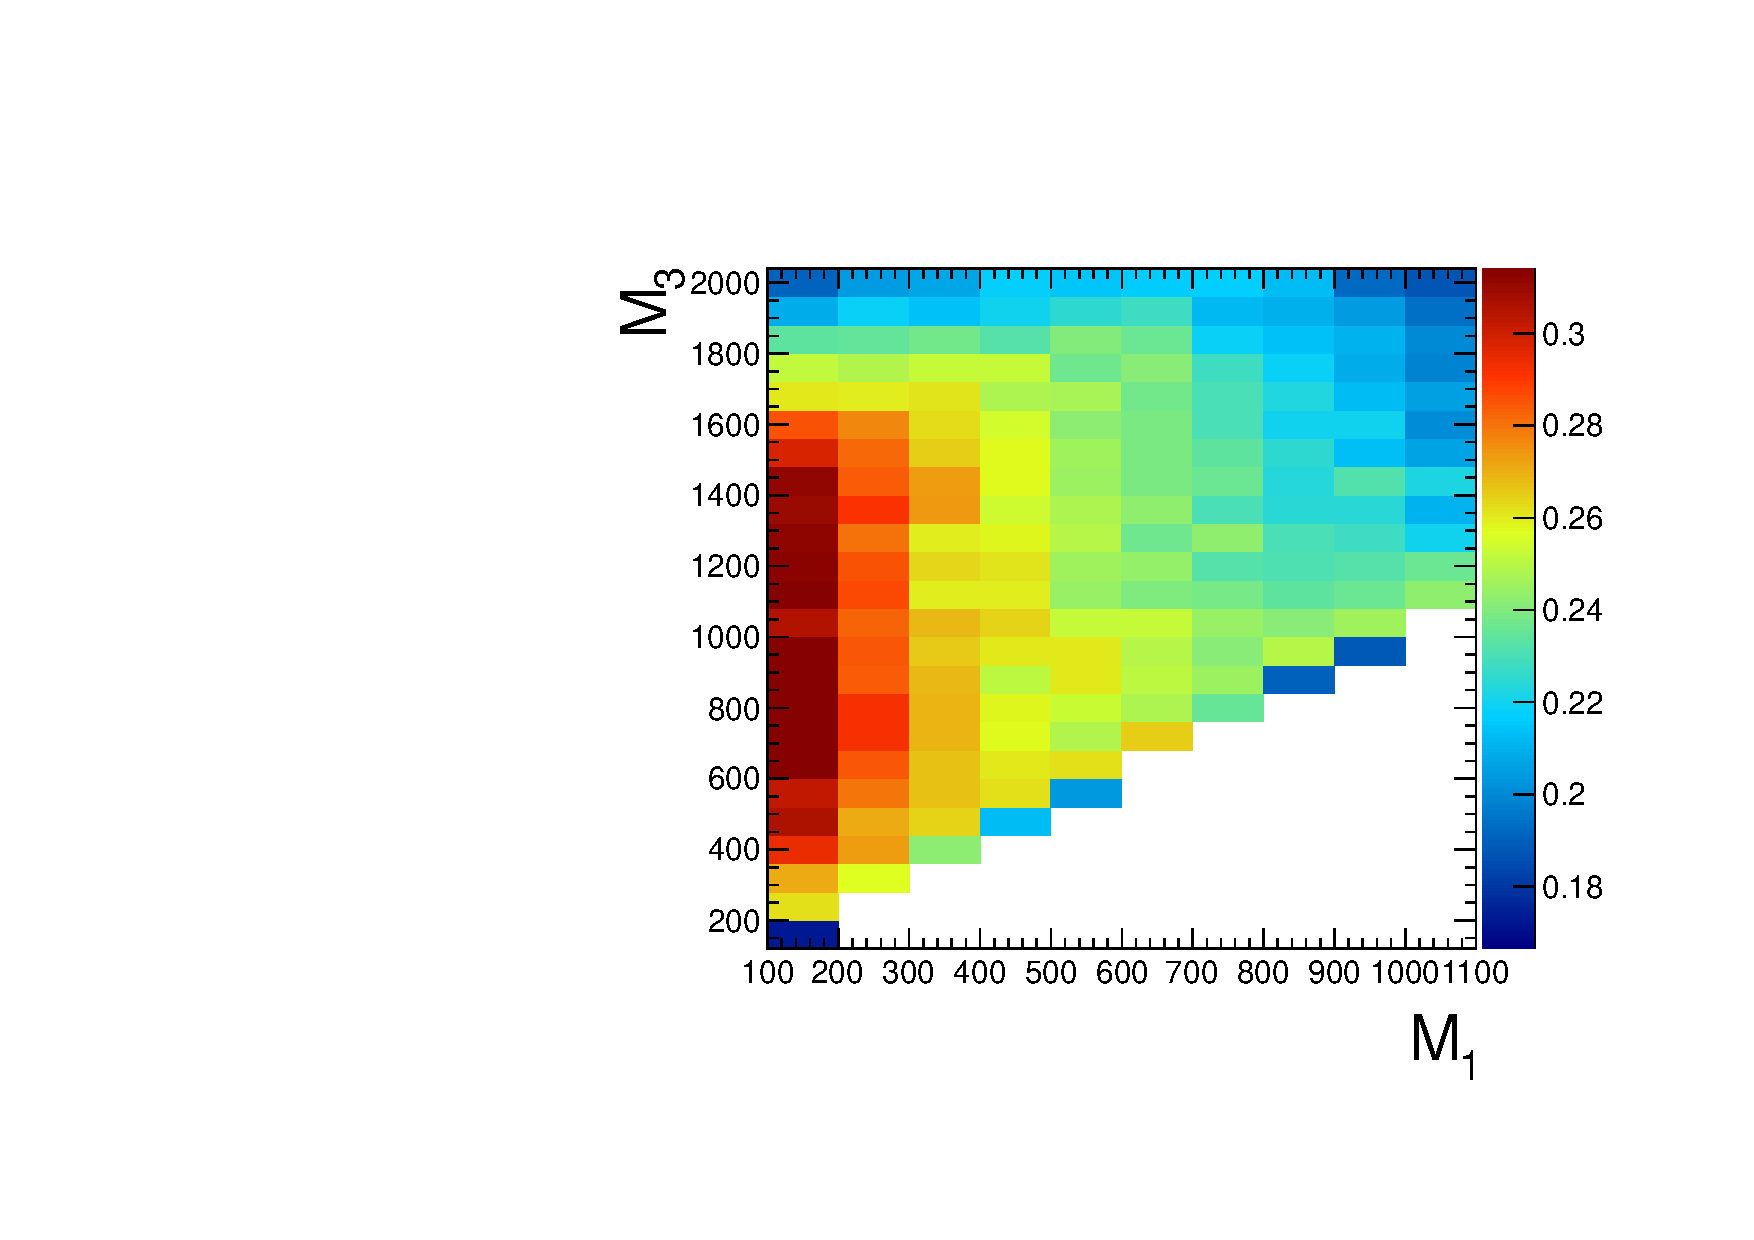
\includegraphics[scale=0.3]{mgluino_vs_mbino_METGeq50GeV_old_1jet}}
	\caption{Signal acceptance $\times$ efficiency (defined in the text) for the three different scenarios described in Sec.~\ref{sec:Simplified Models}.}
	\label{fig:sig_Axe}
\end{figure}

In Figs.~\ref{fig:sig_Axe_mgluino_vs_msquark_bino} and~\ref{fig:sig_Axe_mgluino_vs_msquark_bino_1jet}, the large drop in $\mathcal{A}\times\epsilon$ for $m_{\tilde{q}} > M_{3}$ is due to an increase in the number of jets produced per event and a consequent reduction in the number of photons that pass the $I_{\mathrm{comb}} <$ 6 GeV cut.  For $m_{\tilde{q}} > M_{3}$, there is more phase space available to produce gluinos in the hard scatter than squarks.  However, since gluinos must decay via squarks, and in these models all squarks are heavier than the gluino, only the two-jet decay $\tilde{g}\rightarrow qq\tilde{\chi}^{0}$ is available.  Conversely, when $m_{\tilde{q}} < M_{3}$, there is more phase space available to produce squarks, which may then decay via one jet as $\tilde{q}\rightarrow q\tilde{\chi}^{0}$.  Jets in SUSY events may be very close to the neutralino decay photons, and as a result the photons may fail the strict isolation requirements, leading to lower $\mathcal{A}\times\epsilon$ for jet-rich events.  The worsened acceptance along $M_{3} = 400$ GeV and $m_{\tilde{q}} = 400$ GeV in Fig.~\ref{fig:sig_Axe_mgluino_vs_msquark_bino_1jet} is due to efficiency of the jet cut, which decreases drastically as $M_{3}$ and $m_{\tilde{q}}$ approach $M_{1}$ because of shrinking  phase space to produce hard jets in the squark and gluino decays to neutralinos.

%why does A x e decrease for msquark > ~1600 GeV and mgluino > msquark?
The broad peak in $\mathcal{A}\times\epsilon$ shown in Fig.~\ref{fig:sig_Axe_mgluino_vs_msquark_bino} for $m_{\tilde{q}} < M_{3}$ and $\sim600\mbox{ GeV }<\mbox{ }m_{\tilde{q}}\mbox{ }<\mbox{ }\sim$ 1600 GeV is due to the \MET $>$ 50 GeV cut.  The efficiency of the cut decreases as $m_{\tilde{q}}$ decreases because of the fixed $M_{1}$ of 375 GeV.  If the squark-neutralino mass splitting gets too small, the likelihood of producing an energetic enough gravitino to pass the \MET cut decreases.

$\mathcal{A}\times\epsilon$ is generally much lower for the $M_{2}$ = 375 GeV grid (Figs.~\ref{fig:sig_Axe_mgluino_vs_msquark_wino} and~\ref{fig:sig_Axe_mgluino_vs_msquark_wino_1jet}) due to the larger contribution from chargino decays to $W + \tilde{G}$, which do not give rise to photons in the final state.  The increased acceptance for $M_{3} > m_{\tilde{q}}$ is due to the same jet multiplicity issue affecting the $M_{1}$ = 375 GeV grid.  As $M_{3}$ and $m_{\tilde{q}}$ increase relative to the fixed $M_{2}$, the jets from squark and gluino decay get more energetic, increasing the chance that they will overlap with the neutralino decay photon and cause it to fail the isolation cut.  For $m_{\tilde{q}} \gtrsim$ 1 TeV and $M_{3} \gtrsim$ 800 GeV, the acceptance is so low that not enough events were simulated to see the acceptance decrease over the statistical error.

%why is A x e so high for mgluino = mbino?
%why does A x e drop in the >=1-jet case for M1 ~ 150 GeV, M3 ~> 1600 GeV?  are the jets falling outside acceptance?
In Fig.~\ref{fig:sig_Axe_mgluino_vs_mbino_old}, the neutralino is always heavy enough to guarantee decay to a photon that can pass the 40 GeV $p_{T}$ cut.  $\mathcal{A}\times\epsilon$ increases as $M_{3}$ increases because the larger gluino-neutralino mass splitting gives the neutralino a larger kinetic energy, increasing the chance that it will decay to a photon with 40 GeV $p_{T}$ or higher.  After the bino mass increases beyond the threshold needed to produce high $p_{T}$ photons, $\mathcal{A}\times\epsilon$ decreases with increasing $M_{1}$, independent of gluino mass, because higher $M_{1}$ means more phase space is open to decays of the form $\NLSP\rightarrow Z\tilde{G}$ and $\NLSP\rightarrow H\tilde{G}$.  The two-photon search is naturally not as efficient for these decays.

%explanation of WB scan
%In the $M_{2}$-$M_{1}$ plane, $\mathcal{A}\times\epsilon$ is highest when $M_{2} \gg M_{1}$ and $M_{1}$ is low enough for neutralino decays to photons to dominate (over decays to $Z$ or $H$).  This scenario is what the two-photon search is optimized for.  For large $M_{2}$, $\mathcal{A}\times\epsilon$ decreases as $M_{1}$ increases due to the increasing phase space for neutralino decays to $Z$ and $H$.  For low $M_{1}$, $\mathcal{A}\times\epsilon$ decreases as $M_{2}$ decreases because lowering $M_{2}$ makes the lightest chargino light enough to play a role as co-NLSP in LHC collisions (cf. Sec.~\ref{sec:Phenomenology of General Gauge Mediation}).  In the co-NLSP scenario, the chargino will decay to a $W$ boson and a gravitino, squeezing out phase space for neutralino decays to photons.

\marginpar{\textcolor{blue}{Added signal contamination par.}}There is a small chance that some real GMSB signal events could be reconstructed as $\mathit{ff}$ events in the data.  To correct the signal acceptance for this effect, the number of signal events reconstructed as $\mathit{ff}$ events is subtracted from the number of signal $\gamma\gamma$ events, effectively reducing the signal acceptance.  This is generally a small correction ($\sim5$\%).

\subsection{$\mbox{CL}_{s}$ and the Profile Likelihood Test Statistic}
\label{sec:CLs and the Profile Likelihood Test Statistic}

The process of setting a cross section upper limit entails (1) defining a test statistic, (2) generating a distribution for that test statistic under the signal + background and background-only hypotheses, and (3) deciding whether or not the observed value of the test statistic is more compatible with the signal + background (i.e. weaker upper limit) or background-only (i.e. stronger upper limit) hypotheses by considering where it falls within the test statistic distributions.  An important requirement on the choice of test statistic is that it be able to effectively discriminate between the signal + background and background-only hypotheses, i.e. the shape of its distribution for these two hypotheses should be different.  The procedure for determining the excludability of a particular model given the value of the test statistic observed should not give rise to pathological behavior in the presence of small signals, low statistics, or weak sensitivity to models, as is commonly the case in high energy physics.  These demands on the test statistic and the limit setting procedure itself dictate the choice of the profile likelihood test statistic and $\mbox{CL}_{s}$ procedure.

In the remainder of this section, the notation is taken from ref. \cite{CMS-NOTE-2011/005}.

\subsubsection{Profile Likelihood}
\label{sec:Profile Likelihood}

For a specific model of GMSB, the limit setting procedure concerns the question of whether to reject the signal + background hypothesis $\mu s + b$ in favor of the background-only (Standard Model) hypothesis of $b$ ($\mu$ = 0).  $\mu$ is a dimensionless signal strength parameter.  $s$ is the expected number of signal events, calculated from MC simulated signal events as in Secs.~\ref{sec:Simplified Models} and~\ref{sec:Signal Acceptance Times Efficiency}.  $b$ is the expected number of background events, estimated in Chap.~\ref{chap:Data Analysis}.  By the Neyman-Pearson lemma \cite{Neyman_Pearson}, the ratio of the likelihood of $\mu s + b$ to the likelihood of $b$ is the test statistic with the highest power to reject $\mu s + b$ at whatever confidence level is desired.  In practice, this means that the likelihood ratio is the best discriminator between the GMSB and Standard Model hypotheses.

The likelihood of the signal + background hypothesis as a function of the data (either real or generated) is defined as 

\begin{eqnarray}
\label{eq:L_sb}
\mathcal{L}(\mbox{data} | \mu, \theta) &=& \prod_{i = 1}^{N} \frac{(\mu s_{i}(\theta) + b_{i}(\theta))^{n_{i}}}{n_{i}!}e^{-\mu s_{i}(\theta) - b_{i}(\theta)}p(\tilde{\theta} | \theta)
\end{eqnarray}
%
where $N$ = 5 is the number of \MET bins used in the analysis ([50, 60) GeV, [60, 70) GeV, [70, 80) GeV, [80, 100) GeV, and [100, $\infty$) GeV); $s_{i}(\theta)$ and $b_{i}(\theta)$ are the expected number of signal and background events in \MET bin $i$, respectively; $n_{i}$ is the number of events observed in \MET bin $i$; and $\theta$ represents all the nuisance parameters (uncertainties).  $p(\tilde{\theta} | \theta)$ represents the product of probability distribution functions (PDFs) for the nuisance parameters, where $\tilde{\theta}$ is the default value of the nuisance parameter.  In this analysis, there are eight experimental nuisance parameters per \MET bin, given here as relative errors on the expected number of signal events:

\begin{itemize}
\item Uncertainty on the measured integrated luminosity (4.5\% in all bins) \cite{CMS_PAS_EWK-11-001}
\item Uncertainty on the signal acceptance due to $\epsilon_{e}^{\mathrm{data}}/\epsilon_{e}^{\mathrm{MC}}$ and the pixel veto efficiency error (cf. Sec.~\ref{sec:Photon_Efficiency_Scale_Factor}) (8\% in all bins)
\item Uncertainty on the signal acceptance due to imperfect pileup simulation (2.6\% in all bins)
\item Systematic uncertainty on QCD background prediction due to difference between $\mathit{ff}$ and $ee$ estimates (5.5\%-53\% of the QCD background depending on bin)
\item Systematic uncertainty on electroweak background prediction due to $p_{T}$ dependence of $f_{e\rightarrow\gamma}$ (29\%-30\% of the electroweak background depending on bin)
%high stat. errors for high mq~, high mg~ wino-like grid where analysis is not very sensitive, or lower MET bins for high mg~ in gluino-bino grid
\item Statistical uncertainty on the signal acceptance (1.8\%-100\% depending on model and bin)
\item Statistical uncertainty on the QCD background prediction (7.2\%-38\% of the QCD background depending on bin)
\item Statistical uncertainty on the electroweak background prediction (3.6\%-7.2\% of the electroweak background depending on bin)
\end{itemize}
%
and one very small theoretical nuisance parameter: the uncertainty on the signal acceptance due to underlying parton distribution function (PDF) uncertainties.  In the limit-setting code, the uncertainties on signal acceptance due to photon efficiency and PDF errors are added in quadrature and treated as one.  The uncertainty on the signal acceptance due to jet energy correction uncertainties is negligible, due to the presence of many hard jets in GMSB signal events.  The uncertainties on integrated luminosity and pileup are 100\% correlated between \MET bins, and the uncertainty on signal acceptance can usually be treated similarly because the error on $\epsilon_{e}^{\mathrm{data}}/\epsilon_{e}^{\mathrm{MC}}$ often dominates the PDF error on acceptance (although these three uncertainties are 0\% correlated with each other).

To estimate the uncertainty due to imperfect simulation of LHC pileup, the square of the average data efficiency for photons over the range 1-15 reconstructed primary vertices (see Fig.~\ref{fig:eff_vs_NPV}), weighted by the number of $\gamma\gamma$ events per primary vertex bin, is calculated.  The efficiency per primary vertex bin is estimated from a linear fit to Fig.~\ref{fig:eff_vs_NPV}.  The process is repeated for MC using the entire range of primary vertices in Fig.~\ref{fig:eff_vs_NPV} (all MC signal points have the same pileup simulation).  The error is taken as 2 $\times$ $|$ avg. data efficiency squared - avg. MC efficiency squared $|$/(avg. data efficiency squared + avg. MC efficiency squared).

Each nuisance parameter PDF is modeled by a log-normal distribution:

\begin{eqnarray}
\label{eq:log-normal}
p(\tilde{\theta} | \theta) &=& \frac{1}{\sqrt{2\pi}\ln\kappa} \exp(-\frac{(\ln\tilde{\theta}/\theta)^{2}}{2(\ln\kappa)^{2}})\frac{1}{\tilde{\theta}}
\end{eqnarray}
%
where $\tilde{\theta}$ = 1 and $\kappa$ = 1 + the one-standard-deviation relative error on the nuisance parameter (e.g. for the 4.5\% error due to integrated luminosity, $\kappa$ = 1.045).

Similarly, the likelihood of the background-only hypothesis as a function of the data (either real or generated) is defined as 

\begin{eqnarray}
\label{eq:L_b}
\mathcal{L}(\mbox{data} | 0, \theta) &=& \prod_{i = 1}^{N} \frac{b_{i}(\theta)^{n_{i}}}{n_{i}!}e^{- b_{i}(\theta)}p(\tilde{\theta} | \theta)
\end{eqnarray}

The profile likelihood test statistic is defined as 

\begin{eqnarray}
\label{eq:profile_likelihood}
\tilde{q}_{\mu} &=& -2\ln\frac{\mathcal{L}(\mbox{data} | \mu, \hat{\theta}_{\mu})}{\mathcal{L}(\mbox{data} | \hat{\mu}, \hat{\theta})}, 0 \leq \hat{\mu} \leq \mu
\end{eqnarray}
%
where the $\hat{\theta}_{\mu}$ maximize $\mathcal{L}(\mbox{data} | \mu, \hat{\theta}_{\mu})$ when it is evaluated at a particular $\mu$, and $\hat{\mu}$ and $\hat{\theta}$ are the global maximum likelihood estimators of $\mu$ and $\theta$.  The condition $\hat{\mu} \leq \mu$ insures that the obtained cross section upper limit is one-sided, i.e. there is no possibility to find a lower limit on the cross section.  The profile likelihood test statistic has the nice property that in the asymptotic (large statistics) limit its PDF can be approximated by analytic formulae, eliminating the need to generate multiple toy experiments to get the PDF.  However, the approximation breaks down for small numbers of observed events, so in practice the asymptotic limit is only used as a first guess at the location of the true limit.

The PDFs $f(\tilde{q}_{\mu} | \mu, \hat{\theta}_{\mu}^{\mathrm{obs}})$ and $f(\tilde{q}_{\mu} | 0, \hat{\theta}_{0}^{\mathrm{obs}})$ for the profile likelihood test statistic under the signal + background and background-only hypotheses, respectively, are obtained by generating toy MC pseudo-experiments.  $\hat{\theta}_{\mu}^{\mathrm{obs}}$ and $\hat{\theta}_{0}^{\mathrm{obs}}$ maximize Eqs.~\ref{eq:L_sb} and~\ref{eq:L_b}, respectively, when they are evaluated for the observed data.  For each $\mu$ (and the background-only hypothesis $\mu$ = 0), the pseudo-experiments are generated by picking random values of $s$ and $b$ from a Poisson distribution with the $\theta$ fixed as just described.

\subsubsection{$\mbox{CL}_{s}$}
\label{sec:CLs}

In the classical frequentist approach, a signal model may be excluded at the 95\% confidence level (CL) if the probability of any measurement of the test statistic to be greater than or equal to the observed value given the signal + background hypothesis is 5\%.  This means that the observed value of the test statistic is so incompatible with what one would expect to observe if the signal model were true that, under the assumption that the signal model \textit{is} true, the chance of observing a test statistic even further afield from the signal expectation is only 5\%.  Mathematically, 

\begin{eqnarray}
\label{eq:CLsb_p_value}
p_{\mu} &\equiv& P(\tilde{q}_{\mu} \geq \tilde{q}_{\mu}^{\mathrm{obs}} | \mu s + b) = \int_{\tilde{q}_{\mu}^{\mathrm{obs}}}^{\infty} f(\tilde{q}_{\mu} | \mu, \hat{\theta}_{\mu}^{\mathrm{obs}}) d\tilde{q}_{\mu} \\
p_{\mu} &\leq& 0.05 \Rightarrow \mbox{exclude }\mu \nonumber
\end{eqnarray}
%
where $\tilde{q}_{\mu}^{\mathrm{obs}}$ is the observed value of the test statistic and $p_{\mu}$ is the p-value.  As indicated in Eq.~\ref{eq:CLsb_p_value}, the p-value is simply the integral of the PDF of $\tilde{q}_{\mu}$ from $\tilde{q}_{\mu}^{\mathrm{obs}}$ to infinity.

By construction, the classical 95\% CL frequentist approach described above will reject a true signal + background hypothesis 5\% of the time.  This can happen if the experiment gets ``unlucky" and the observation fluctuates low, causing $\tilde{q}_{\mu}^{\mathrm{obs}}$ to fall in the tail of the $\tilde{q}_{\mu}$ distribution.  This poses a problem for the case of very weak signals ($\mu \sim 0$), because it will lead to spurious exclusions of models to which the experiment has little sensitivity.  To avoid this pitfall, the $\mbox{CL}_{s}$ limit setting method is used.

In the $\mbox{CL}_{s}$ method, the classical frequentist p-value of Eq.~\ref{eq:CLsb_p_value} is simply divided by one minus the p-value of the background-only hypothesis, and it is this ratio, rather than the p-value of the signal + background hypothesis alone, that is required to be $\leq$ 0.05.  Mathematically, 

\begin{eqnarray}
\label{eq:CLb_p_value}
1 - p_{0} &\equiv& P(\tilde{q}_{\mu} \geq \tilde{q}_{\mu}^{\mathrm{obs}} | b) = \int_{\tilde{q}_{\mu}^{\mathrm{obs}}}^{\infty} f(\tilde{q}_{\mu} | 0, \hat{\theta}_{0}^{\mathrm{obs}}) d\tilde{q}_{\mu} \\
\mbox{CL}_{s}(\mu) &\equiv& \frac{p_{\mu}}{1 - p_{0}} \\
\mbox{CL}_{s}(\mu) &\leq& 0.05 \Rightarrow \mbox{exclude }\mu \nonumber
\end{eqnarray}
%
where $p_{0}$ is the p-value for the background-only hypothesis ($\mu$ = 0).  In the case of low sensitivity to $\mu$, $p_{\mu} \lesssim 1 - p_{0}$, so $\mbox{CL}_{s}(\mu) \lesssim$ 1 and $\mu$ will not be excluded.  On the contrary, for high sensitivity to $\mu$ ($\mu s \gg \sigma_{b}$), $p_{\mu} \ll 1 - p_{0}$, so models that can be excluded by the criterion $p_{\mu} \leq$ 0.05 will also be excluded by the criterion $\mbox{CL}_{s} \leq$ 0.05.  Compared to the classical frequentist method, $\mbox{CL}_{s}$ limits can be a little stronger in the case of low signal sensitivity \cite{CMS-NOTE-2011/005}.

To determine the upper limit on the cross section of a particular model, the lowest value of $\mu$ for which $\mbox{CL}_{s}(\mu) \leq$ 0.05, denoted $\mu^{95\%\mathrm{CL}}$, is found.  The cross section upper limit of that model is then simply $\mu^{95\%\mathrm{CL}}$ multiplied by the expected cross section of the model (cf. Fig.~\ref{fig:sig_xsec}).

In contrast to the observed upper limit, the expected upper limit is calculated from an ensemble of background-only MC pseudo-experiments.  The distribution $f(\mu^{95\%\mathrm{CL}}_{\mathrm{pseudo}})$ is plotted (one entry per pseudo-experiment).  The median expected upper limits and $\pm1\sigma$ and $\pm2\sigma$ bands are defined as 

\begin{eqnarray}
\label{eq:exp_limits}
0.5 &=& \int_{0}^{\mu^{95\%\mathrm{CL}}_{\mathrm{,exp}}} f(\mu^{95\%\mathrm{CL}}_{\mathrm{pseudo}})d\mu^{95\%\mathrm{CL}}_{\mathrm{pseudo}} \\
0.16 &=& \int_{0}^{\mu^{95\%\mathrm{CL}}_{-1\sigma\mathrm{,exp}}} f(\mu^{95\%\mathrm{CL}}_{\mathrm{pseudo}})d\mu^{95\%\mathrm{CL}}_{\mathrm{pseudo}} \\
0.84 &=& \int_{0}^{\mu^{95\%\mathrm{CL}}_{+1\sigma\mathrm{,exp}}} f(\mu^{95\%\mathrm{CL}}_{\mathrm{pseudo}})d\mu^{95\%\mathrm{CL}}_{\mathrm{pseudo}} \\
0.025 &=& \int_{0}^{\mu^{95\%\mathrm{CL}}_{-2\sigma\mathrm{,exp}}} f(\mu^{95\%\mathrm{CL}}_{\mathrm{pseudo}})d\mu^{95\%\mathrm{CL}}_{\mathrm{pseudo}} \\
0.975 &=& \int_{0}^{\mu^{95\%\mathrm{CL}}_{+2\sigma\mathrm{,exp}}} f(\mu^{95\%\mathrm{CL}}_{\mathrm{pseudo}})d\mu^{95\%\mathrm{CL}}_{\mathrm{pseudo}}
\end{eqnarray}

The technical procedure followed to calculate the 95\% CL cross section upper limits for each GMSB model tested is given below.

\begin{enumerate}
\item Calculate a guess for the median expected limit and $\pm2\sigma$ error bands ($\mu^{95\%\mathrm{CL}}_{\pm2\sigma\mathrm{,guess}}$) using the asymptotic formulae for $f(\tilde{q}_{\mu} | 0, \hat{\theta}_{0}^{\mathrm{obs}})$.
\item Calculate observed ($\mu^{95\%\mathrm{CL}}_{\mathrm{obs,asym}}$), median expected ($\mu^{95\%\mathrm{CL}}_{\mathrm{exp,asym}}$), and $\pm1\sigma$ ($\mu^{95\%\mathrm{CL}}_{\pm1\sigma\mathrm{,asym}}$) and $\pm2\sigma$ ($\mu^{95\%\mathrm{CL}}_{\pm2\sigma\mathrm{,asym}}$) expected $\mbox{CL}_{s}$ limits using the asymptotic formulae for $f(\tilde{q}_{\mu} | \mu, \hat{\theta}_{\mu}^{\mathrm{obs}})$ and $f(\tilde{q}_{\mu} | 0, \hat{\theta}_{0}^{\mathrm{obs}})$.  Restrict the range of $\mu^{95\%\mathrm{CL}}_{\mathrm{obs,asym}}$ and $\mu^{95\%\mathrm{CL}}_{\mathrm{exp,asym}}$ to $\left[0, 5\times\mu^{95\%\mathrm{CL}}_{\pm2\sigma\mathrm{,guess}}\right]$ (this avoids pathological behavior of the limit-setting code when the expected number of signal events is much greater than the observed number of events and only introduces a $\sim5$\% upward bias in the observed limit, well within the $\pm1\sigma$ error bands).
\item Calculate median expected ($\mu^{95\%\mathrm{CL}}_{\mathrm{exp}}$) and $\pm1\sigma$ ($\mu^{95\%\mathrm{CL}}_{\pm1\sigma}$) and $\pm2\sigma$ ($\mu^{95\%\mathrm{CL}}_{\pm2\sigma}$) expected $\mbox{CL}_{s}$ limits using 100 toy MC pseudo-experiments to generate $f(\tilde{q}_{\mu} | \mu, \hat{\theta}_{\mu}^{\mathrm{obs}})$ and $f(\tilde{q}_{\mu} | 0, \hat{\theta}_{0}^{\mathrm{obs}})$.  Restrict the range of $\mu^{95\%\mathrm{CL}}_{\mathrm{exp}}$ to $\left[0, 5\times\mu^{95\%\mathrm{CL}}_{\pm2\sigma\mathrm{,guess}}\right]$.
\item If $\mu^{95\%\mathrm{CL}}_{\pm2\sigma}$ could not be calculated, set $\mu^{95\%\mathrm{CL}}_{\pm2\sigma} = \mu^{95\%\mathrm{CL}}_{\pm2\sigma\mathrm{,asym}}$ instead.
\item If $\mu^{95\%\mathrm{CL}}_{+2\sigma} \neq \mu^{95\%\mathrm{CL}}_{-2\sigma}$ and $\mu^{95\%\mathrm{CL}}_{\mathrm{obs,asym}} >$ 0.0001:
\begin{itemize}
\item If $\mu^{95\%\mathrm{CL}}_{\mathrm{obs,asym}} > \mu^{95\%\mathrm{CL}}_{+2\sigma}$, set $\mu^{95\%\mathrm{CL}}_{+2\sigma} = 1.3\times\mu^{95\%\mathrm{CL}}_{\mathrm{obs,asym}}$.
\item If $\mu^{95\%\mathrm{CL}}_{\mathrm{obs,asym}} < \mu^{95\%\mathrm{CL}}_{-2\sigma}$, set $\mu^{95\%\mathrm{CL}}_{-2\sigma} = 0.7\times\mu^{95\%\mathrm{CL}}_{\mathrm{obs,asym}}$.
\end{itemize}
\item If $\mu^{95\%\mathrm{CL}}_{+2\sigma} = \mu^{95\%\mathrm{CL}}_{-2\sigma}$, set $\mu^{95\%\mathrm{CL}}_{\pm2\sigma} = \mu^{95\%\mathrm{CL}}_{\pm2\sigma\mathrm{,asym}}$ instead.
\item Scan over 100 equally spaced test values of $\mu$ between $\mu^{95\%\mathrm{CL}}_{-2\sigma}$ and $\mu^{95\%\mathrm{CL}}_{+2\sigma}$ and, if $\mu >$ 0.0001, calculate the $\mbox{CL}_{s}$ p-value ($p_{\mu}$) for this test value of $\mu$ to $10^{-6}$ precision using a minimum of 500 toy experiments to generate $f(\tilde{q}_{\mu} | \mu, \hat{\theta}_{\mu}^{\mathrm{obs}})$ and $f(\tilde{q}_{\mu} | 0, \hat{\theta}_{0}^{\mathrm{obs}})$.
\item Determine the observed ($\mu^{95\%\mathrm{CL}}_{\mathrm{obs,scan}}$), median expected ($\mu^{95\%\mathrm{CL}}_{\mathrm{exp,scan}}$), and $\pm1\sigma$ ($\mu^{95\%\mathrm{CL}}_{\pm1\sigma\mathrm{,scan}}$) and $\pm2\sigma$ ($\mu^{95\%\mathrm{CL}}_{\pm2\sigma\mathrm{,scan}}$) expected $\mbox{CL}_{s}$ limits from the scan p-values for the signal + background and background-only pseudo-experiments.
\end{enumerate}

%%fill in details of GMSB model and make plot
%Figure~\ref{fig:test_statistic_distributions} shows $f(\tilde{q}_{\mu_{<}} | \mu_{<}, \hat{\theta}_{\mu_{<}}^{\mathrm{obs}})$ ($\mu < \mu^{95\%\mathrm{CL}}$), $f(\tilde{q}_{\mu^{95\%\mathrm{CL}}} | \mu^{95\%\mathrm{CL}}, \hat{\theta}_{\mu^{95\%\mathrm{CL}}}^{\mathrm{obs}})$, $f(\tilde{q}_{\mu_{>}} | \mu_{>}, \hat{\theta}_{\mu_{>}}^{\mathrm{obs}})$ ($\mu > \mu^{95\%\mathrm{CL}}$), and $f(\tilde{q}_{\mu} | 0, \hat{\theta}_{0}^{\mathrm{obs}})$ for a GMSB model with \textcolor{red}{\textbf{some parameters}}.  The observed value of the test statistic for each value of $\mu$ is also shown, along with the p-values.

%\begin{figure}
%	\centering
%	\includegraphics[scale=1.0]{test_statistic_distributions}
%	\caption{$f(\tilde{q}_{\mu_{<}} | \mu_{<}, \hat{\theta}_{\mu_{<}}^{\mathrm{obs}})$ ($\mu < \mu^{95\%\mathrm{CL}}$, red), $f(\tilde{q}_{\mu^{95\%\mathrm{CL}}} | \mu^{95\%\mathrm{CL}}, \hat{\theta}_{\mu^{95\%\mathrm{CL}}}^{\mathrm{obs}})$ (black), $f(\tilde{q}_{\mu_{>}} | \mu_{>}, \hat{\theta}_{\mu_{>}}^{\mathrm{obs}})$ ($\mu > \mu^{95\%\mathrm{CL}}$, blue), and $f(\tilde{q}_{\mu} | 0, \hat{\theta}_{0}^{\mathrm{obs}})$ (magenta) for a GMSB model with \textcolor{red}{\textbf{some parameters}}.  The observed value of the test statistic for each value of $\mu$ is also shown, along with the p-values.}
%	\label{fig:test_statistic_distributions}
%\end{figure}

Finally, a particular GMSB model is excluded if the upper limit on the cross section for that model is less than the expected theoretical cross section.

\section{Cross Section Upper Limits}
\label{sec:Cross Section Upper Limits}

Figure~\ref{fig:xsec_UL} shows the observed upper limits on the cross sections for the models described in Sec.~\ref{sec:Simplified Models}.  In some ($\mathcal{O}(10^{-3})$) cases, the upper limit is zero due to a computational failure.  The upper limit for these points is estimated from the average of the upper limits of the four neighboring points, as shown in Figure~\ref{fig:UL_estimation_points}.  If any of the four points is also missing a valid upper limit, it is dropped from the average.  The errors on the individual upper limits used in the estimate are propagated to the error on the average.

\begin{figure}
	\centering
	\subfloat[$M_{2}$ decoupled ($M_{2}$ = 3.5 TeV), $M_{1}$ = 375 GeV, $M_{3}$ vs. $m_{\tilde{q}}$, $\geq0$ jets.]{\label{fig:xsec_UL_mgluino_vs_msquark_bino}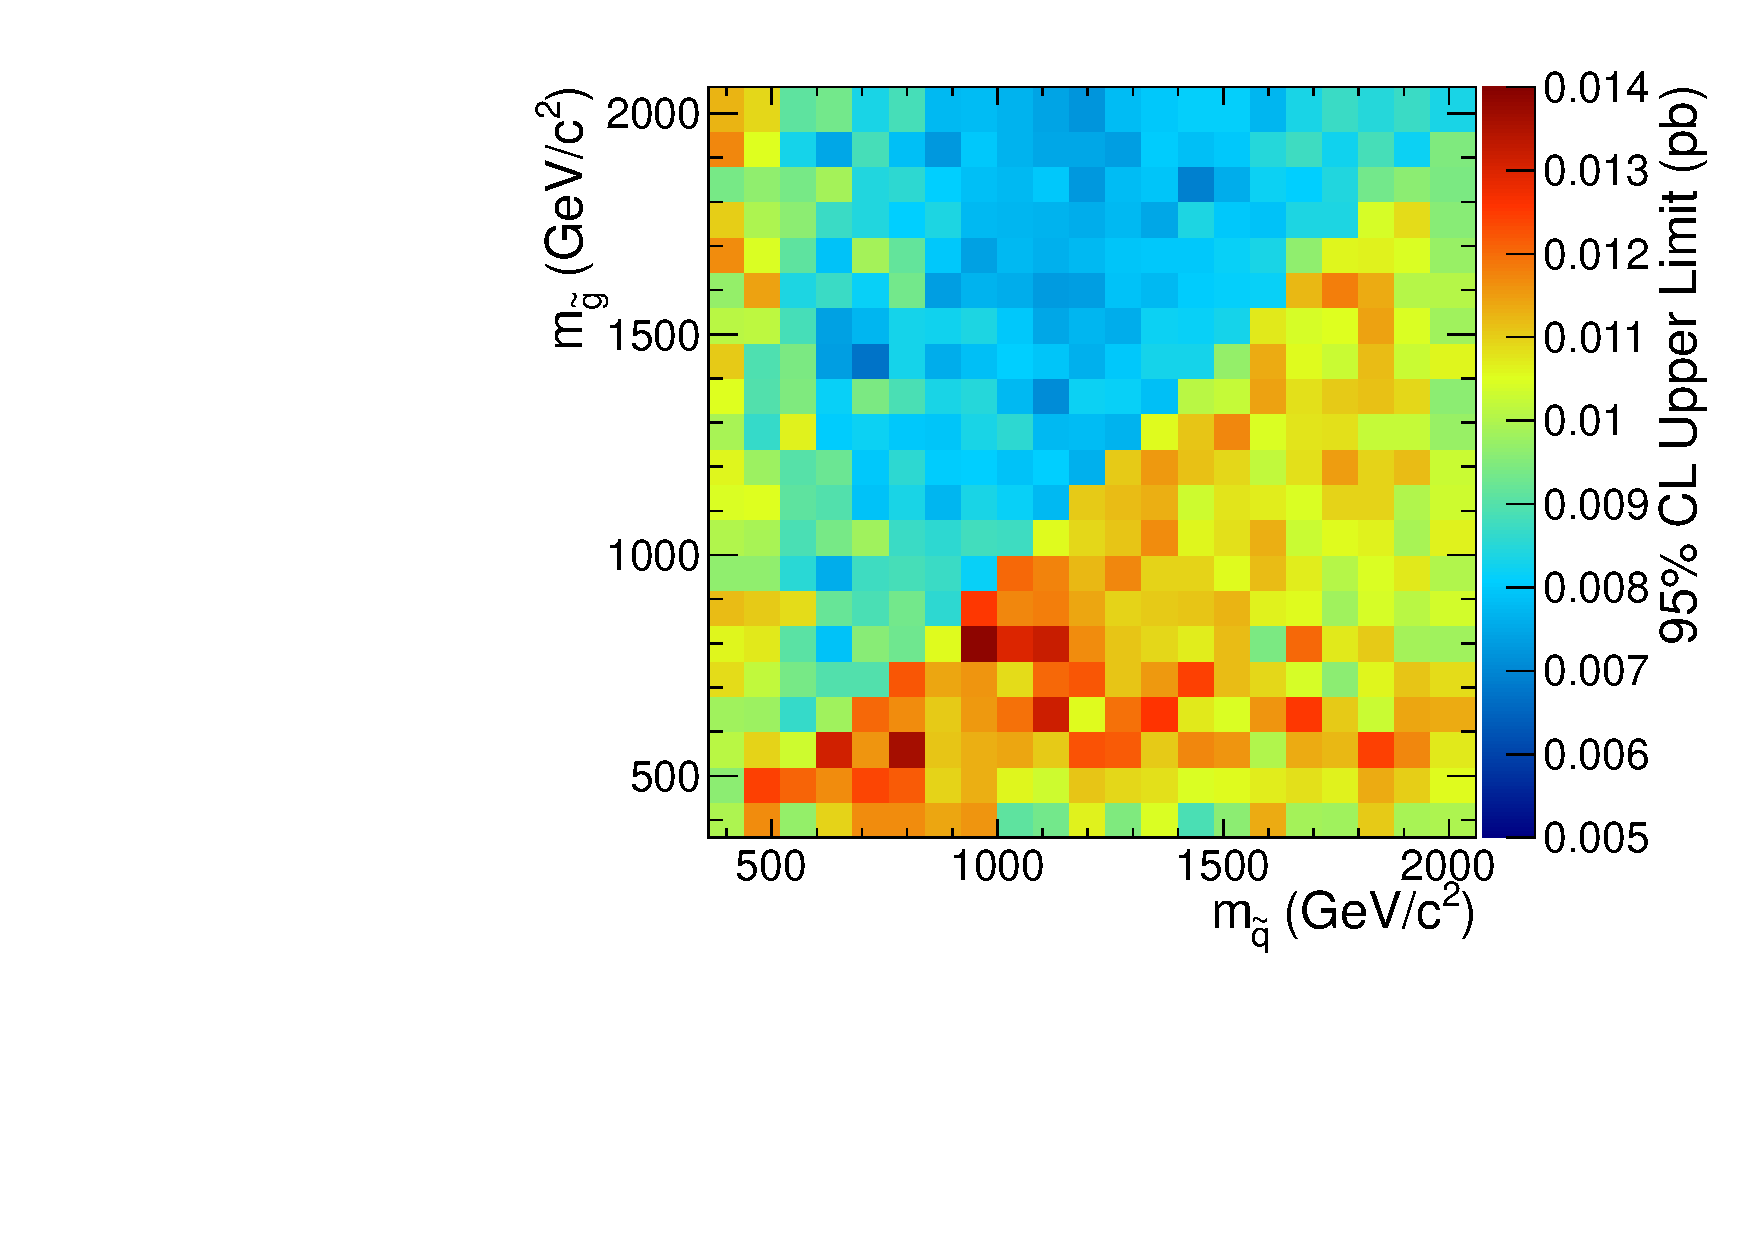
\includegraphics[scale=0.3]{can_limit_bino_mN375_met100_nojet}}
	\hspace{1cm}
	\subfloat[$M_{2}$ decoupled ($M_{2}$ = 3.5 TeV), $M_{1}$ = 375 GeV, $M_{3}$ vs. $m_{\tilde{q}}$, $\geq1$ jet.]{\label{fig:xsec_UL_mgluino_vs_msquark_bino_1jet}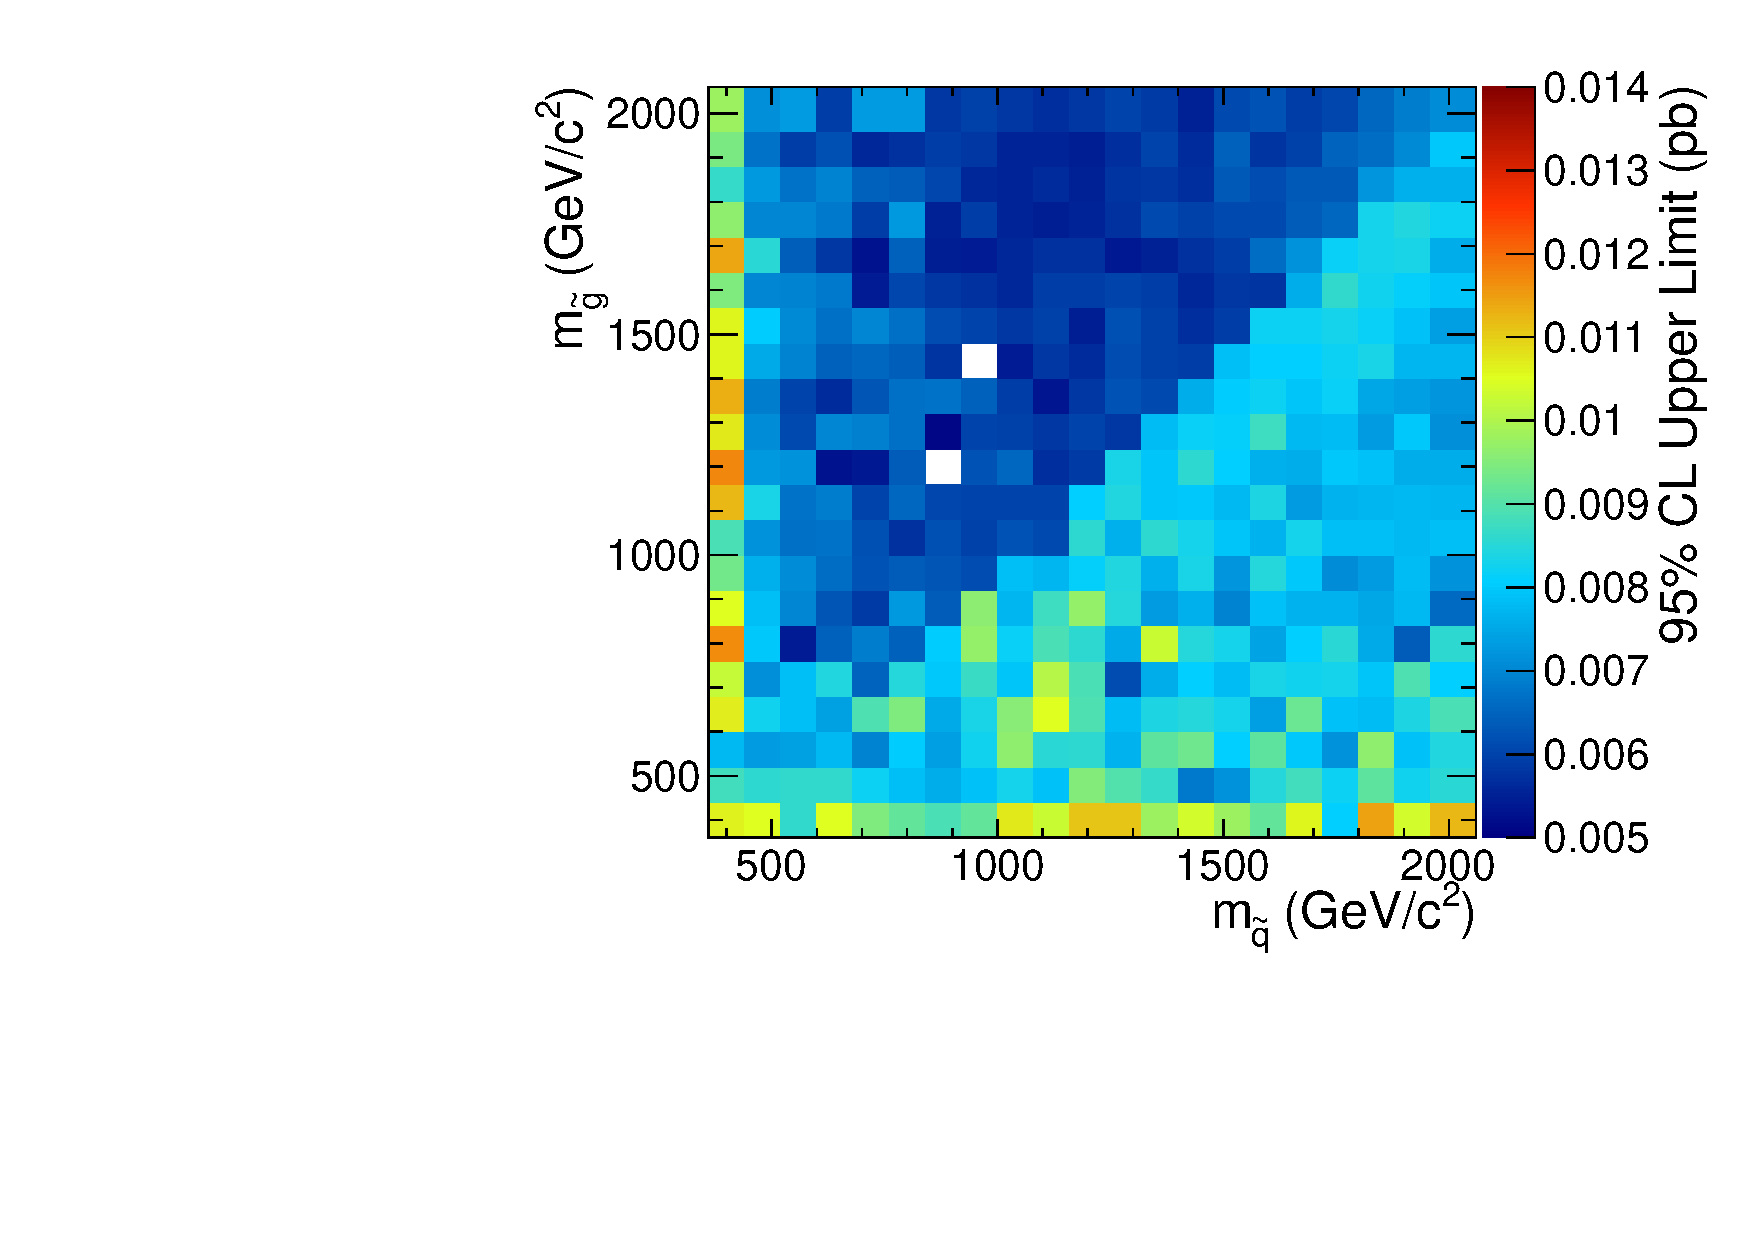
\includegraphics[scale=0.3]{can_limit_bino_mN375_met100_1jet}}
	\\
	\subfloat[$M_{1}$ decoupled ($M_{1}$ = 3.5 TeV), $M_{2}$ = 375 GeV, $M_{3}$ vs. $m_{\tilde{q}}$, $\geq0$ jets.]{\label{fig:xsec_UL_mgluino_vs_msquark_wino}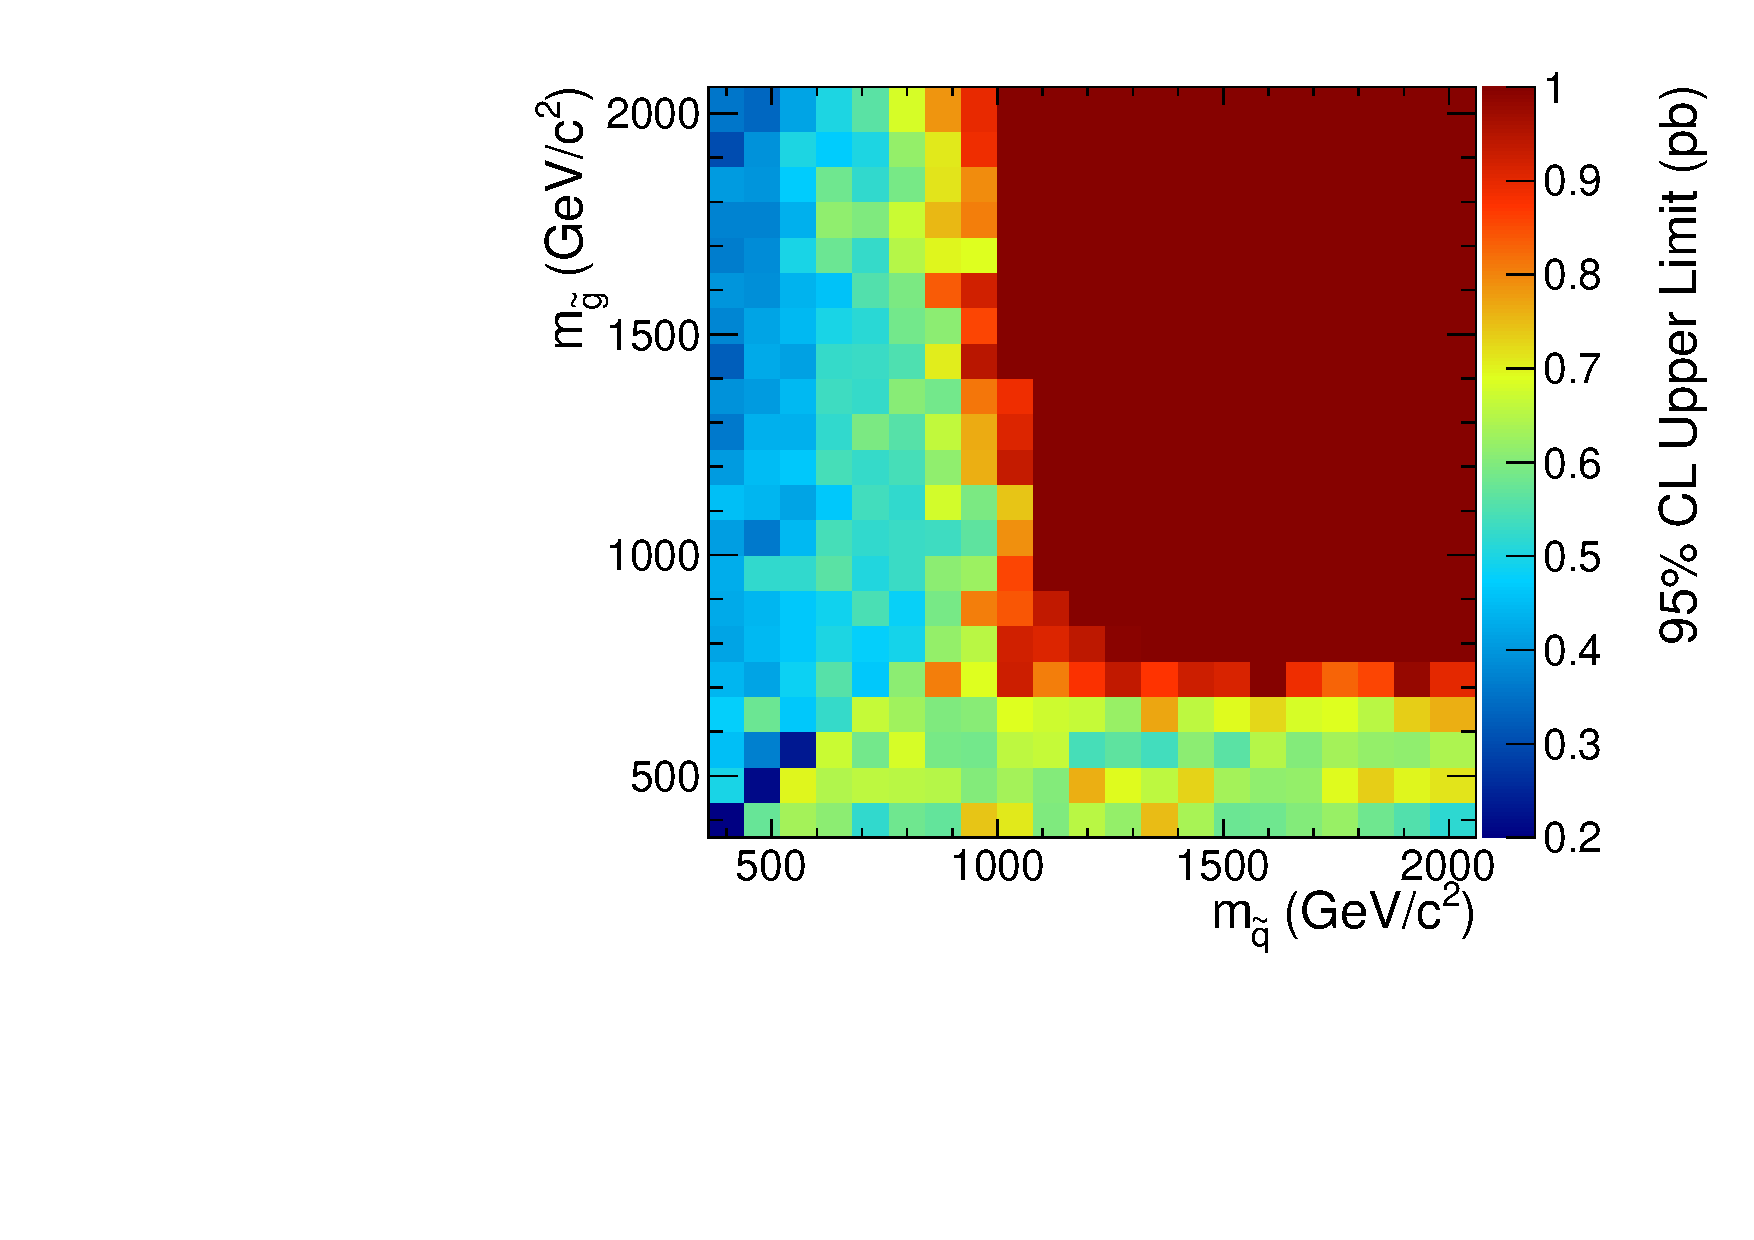
\includegraphics[scale=0.3]{can_limit_wino_mN375_met100_nojet}}
	\hspace{1cm}
	\subfloat[$M_{1}$ decoupled ($M_{1}$ = 3.5 TeV), $M_{2}$ = 375 GeV, $M_{3}$ vs. $m_{\tilde{q}}$, $\geq1$ jet.]{\label{fig:xsec_UL_mgluino_vs_msquark_wino_1jet}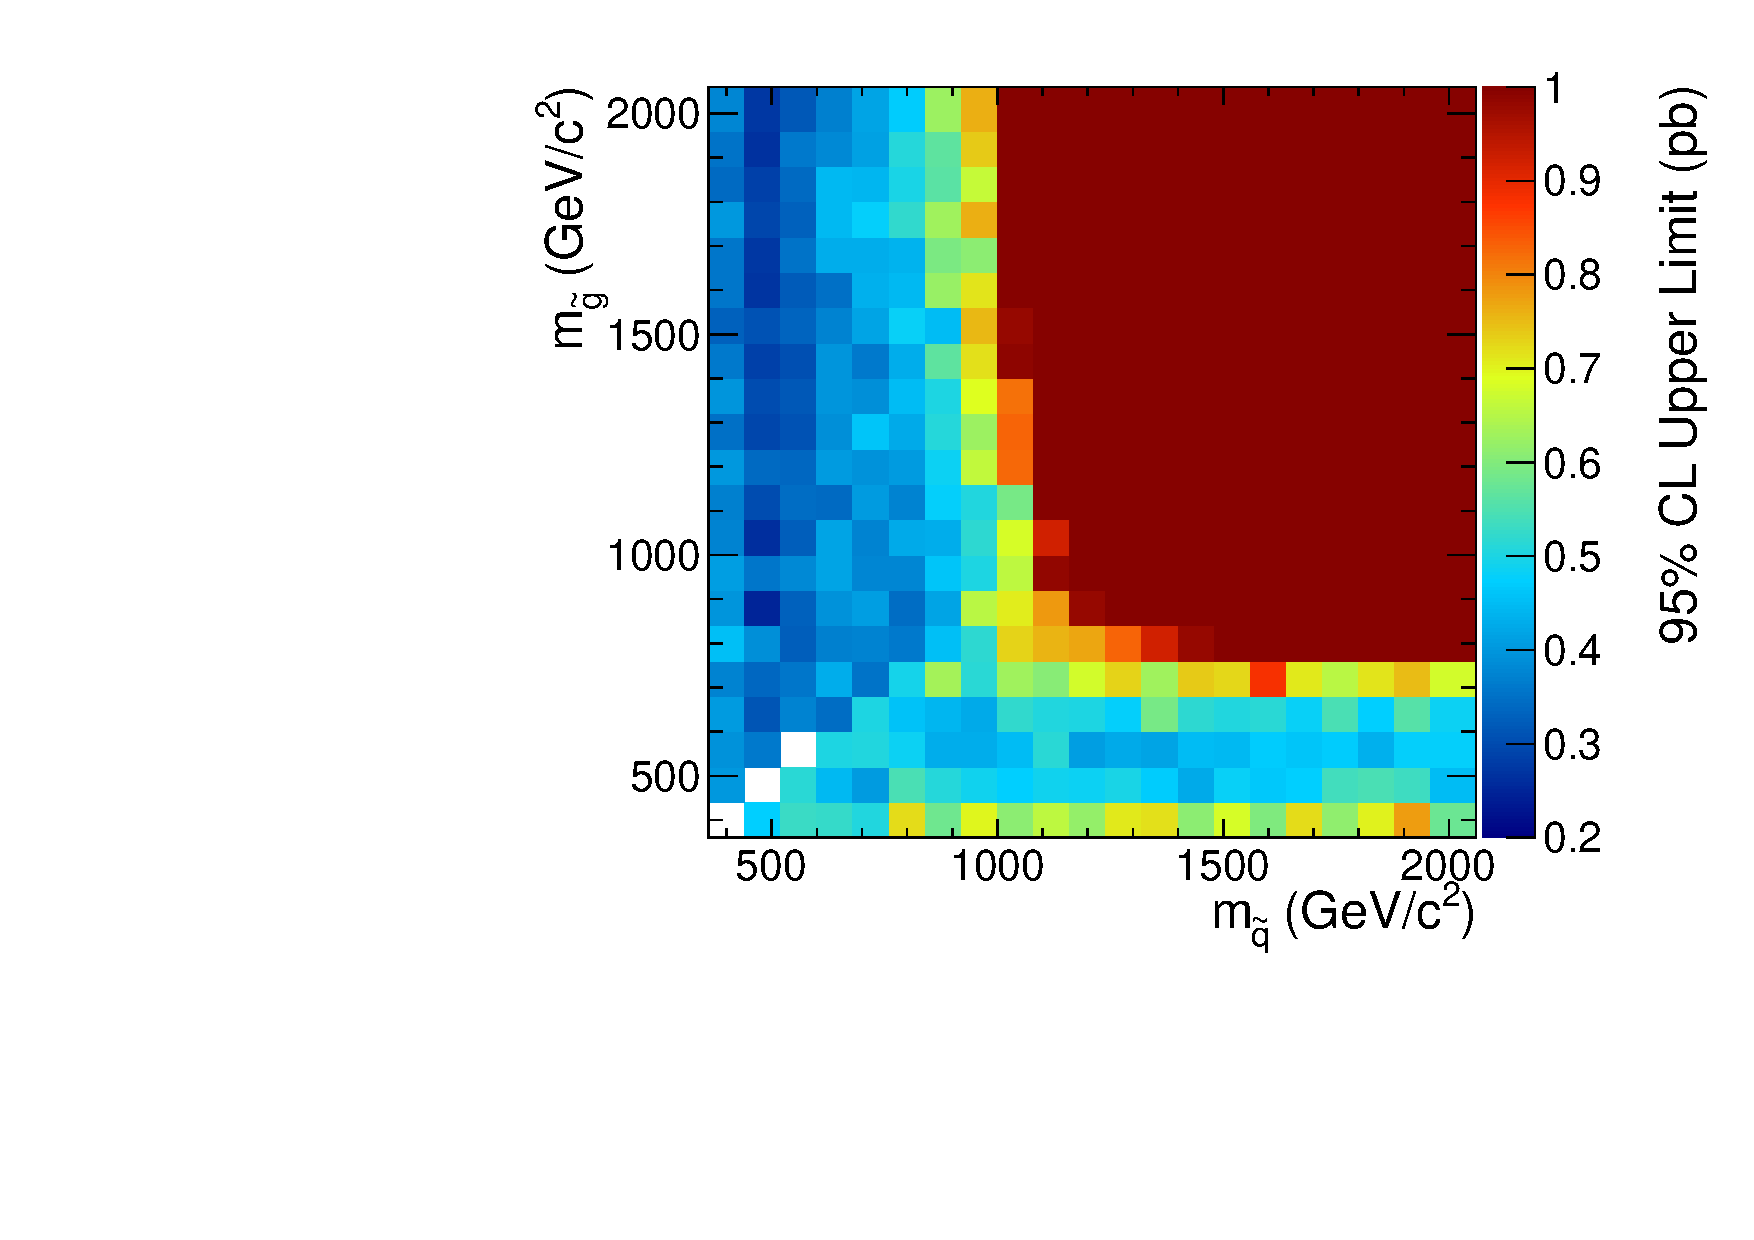
\includegraphics[scale=0.3]{can_limit_wino_mN375_met100_1jet}}
	\\
	\subfloat[$m_{\tilde{q}}$ decoupled ($m_{\tilde{q}}$ = 2.5 TeV), $M_{3}$ vs. $M_{1}$, $\geq0$ jets.]{\label{fig:xsec_UL_mgluino_vs_mbino_old}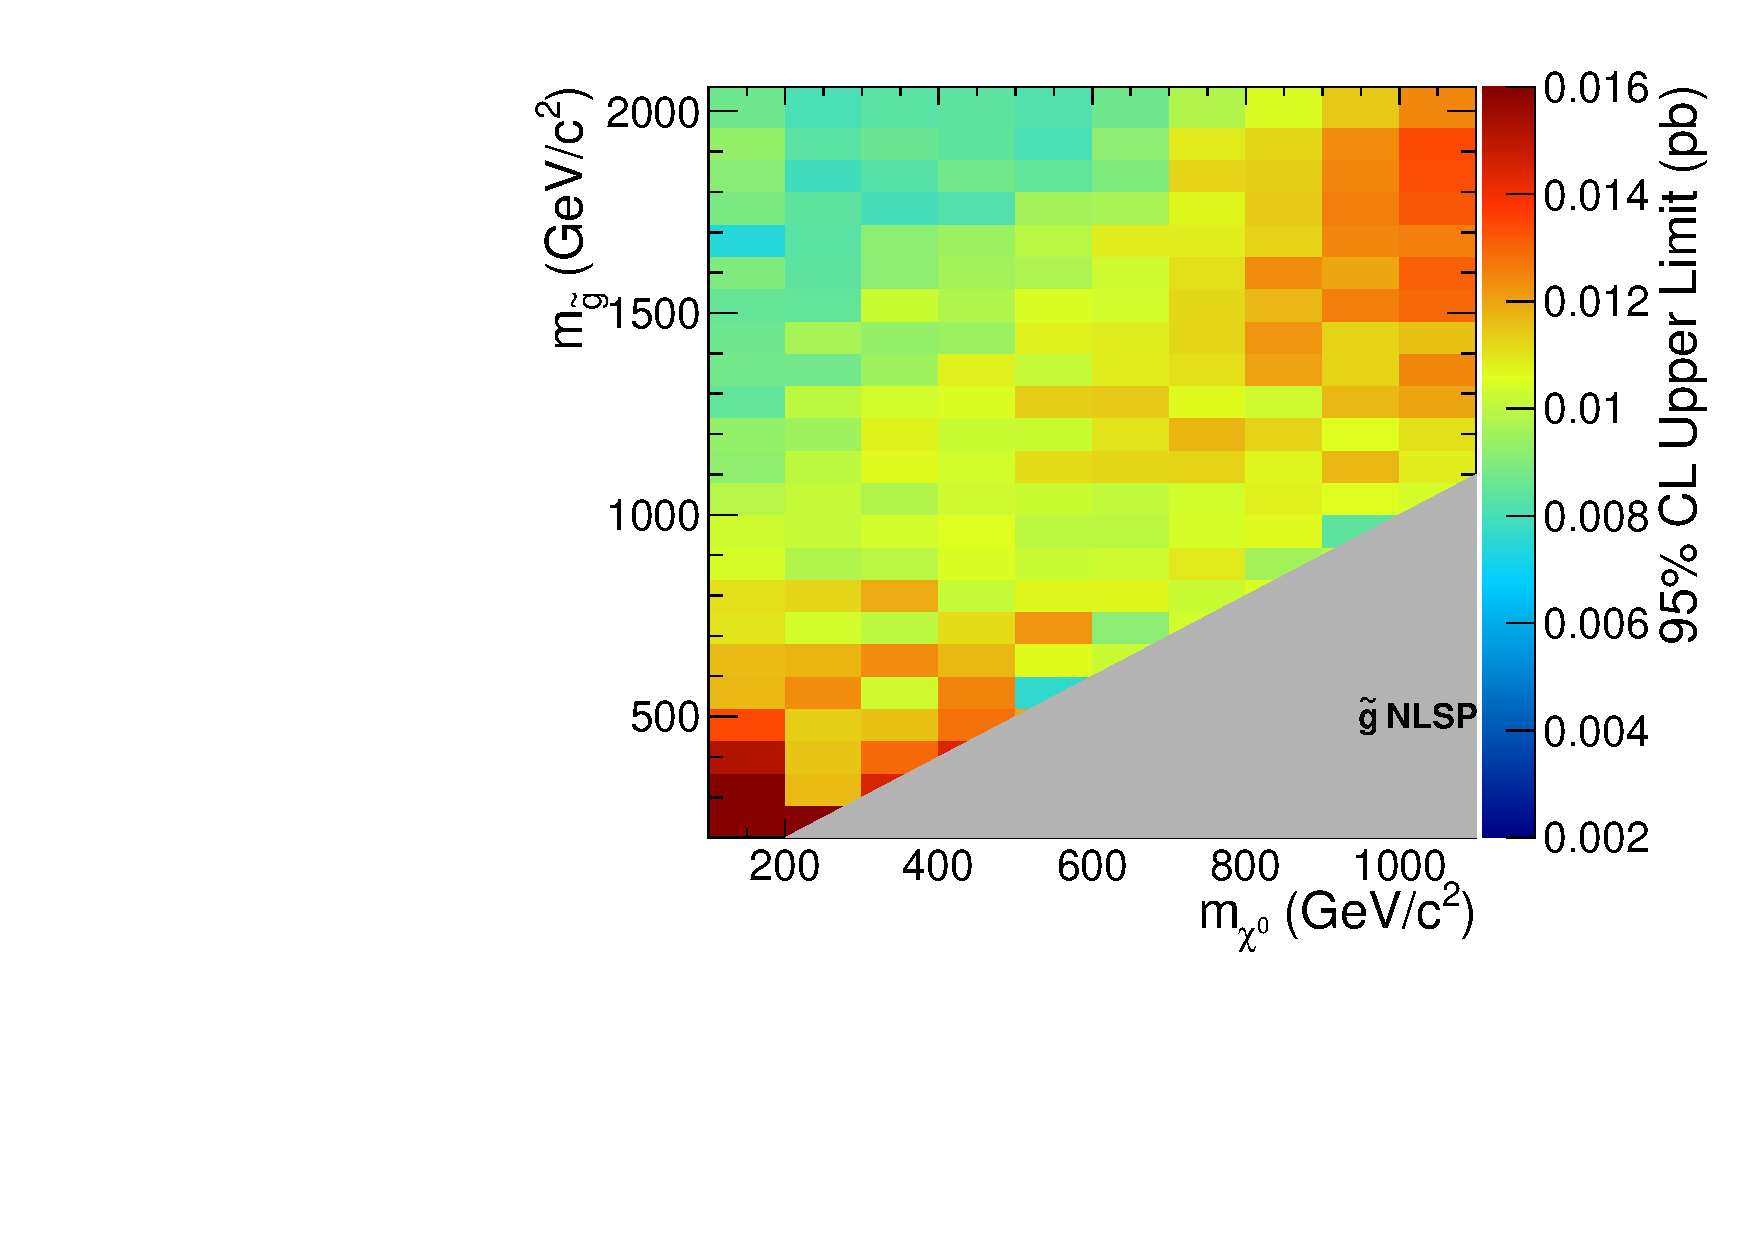
\includegraphics[scale=0.3]{can_limit_bino_mNScan_met100_nojet}}
	\hspace{1cm}
	\subfloat[$m_{\tilde{q}}$ decoupled ($m_{\tilde{q}}$ = 2.5 TeV), $M_{3}$ vs. $M_{1}$, $\geq1$ jet.]{\label{fig:xsec_UL_mgluino_vs_mbino_old_1jet}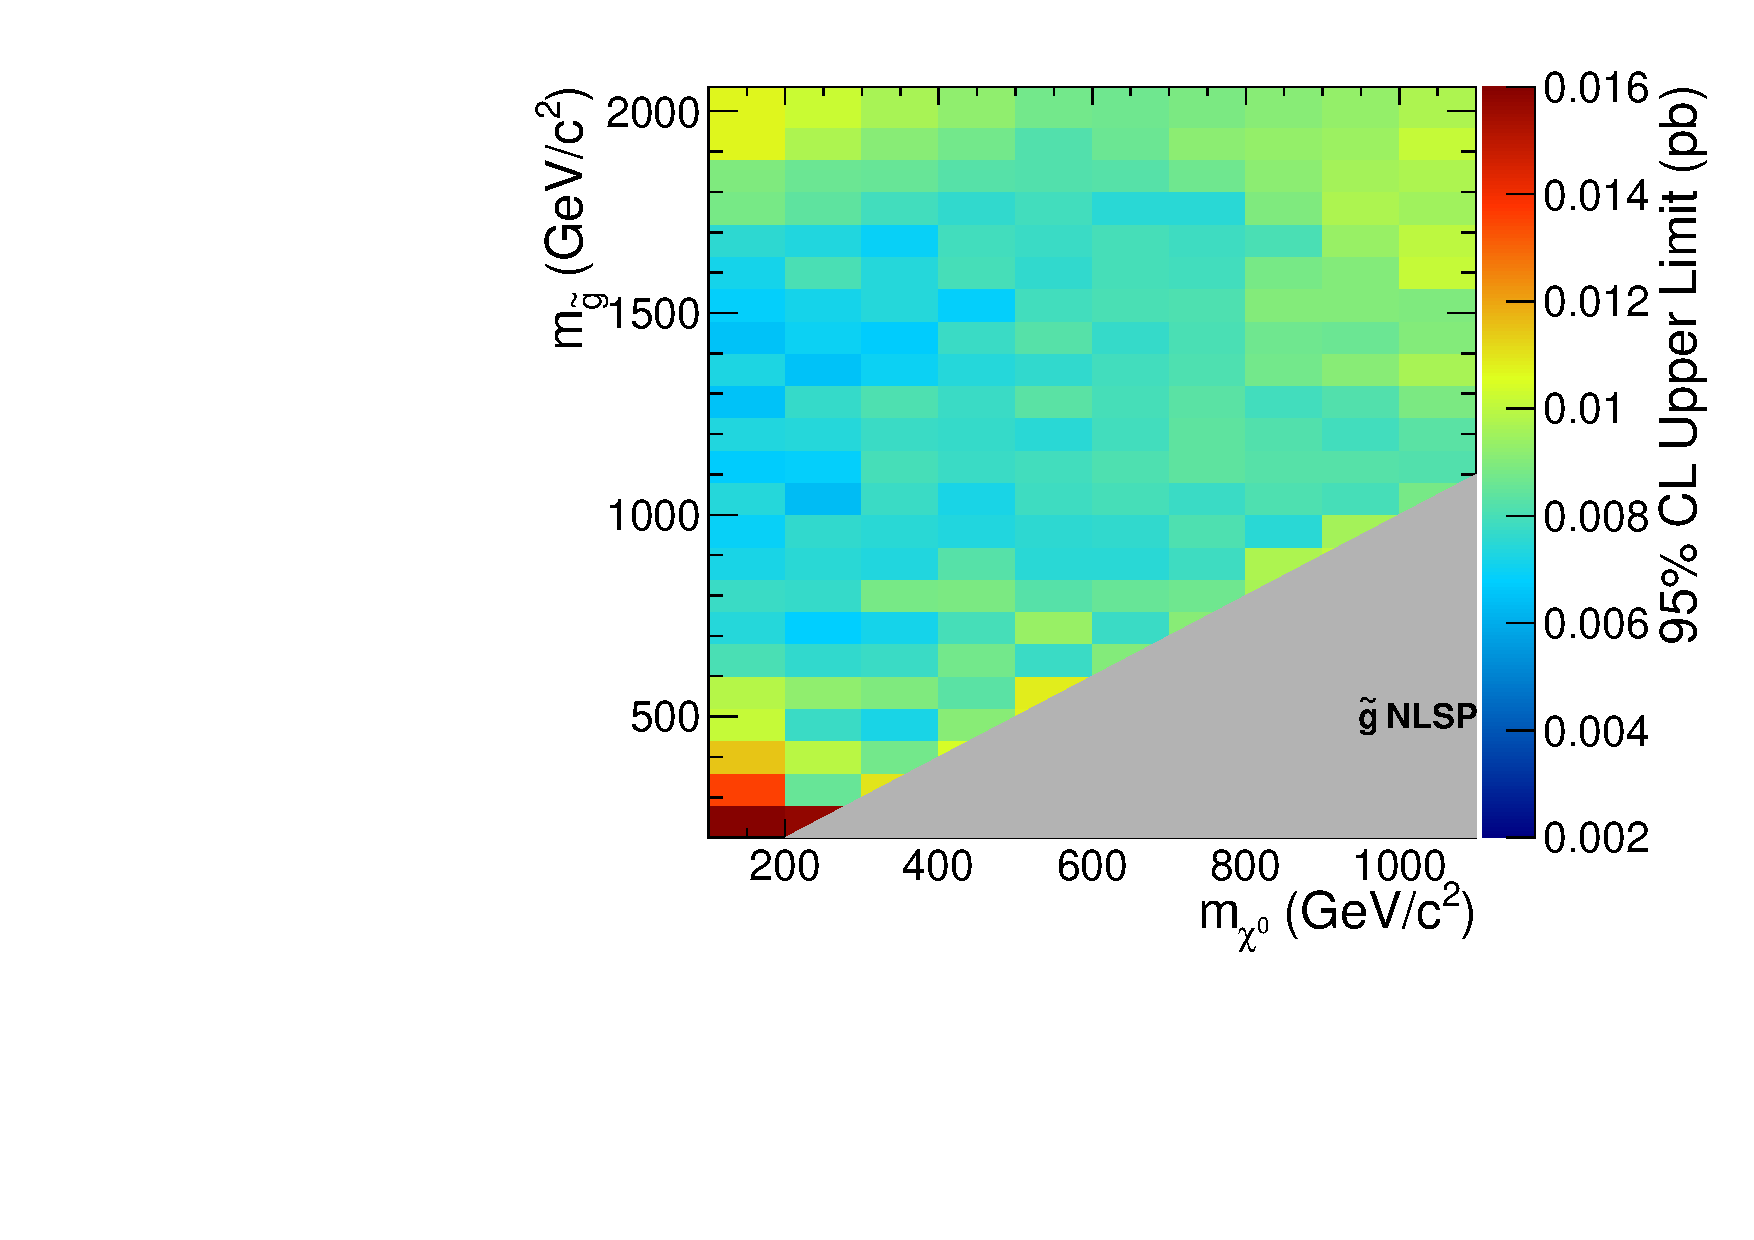
\includegraphics[scale=0.3]{can_limit_bino_mNScan_met100_1jet}}
	\caption{Cross section upper limits for the three different scenarios described in Sec.~\ref{sec:Simplified Models}.}
	\label{fig:xsec_UL}
\end{figure}

\begin{figure}
	\centering
	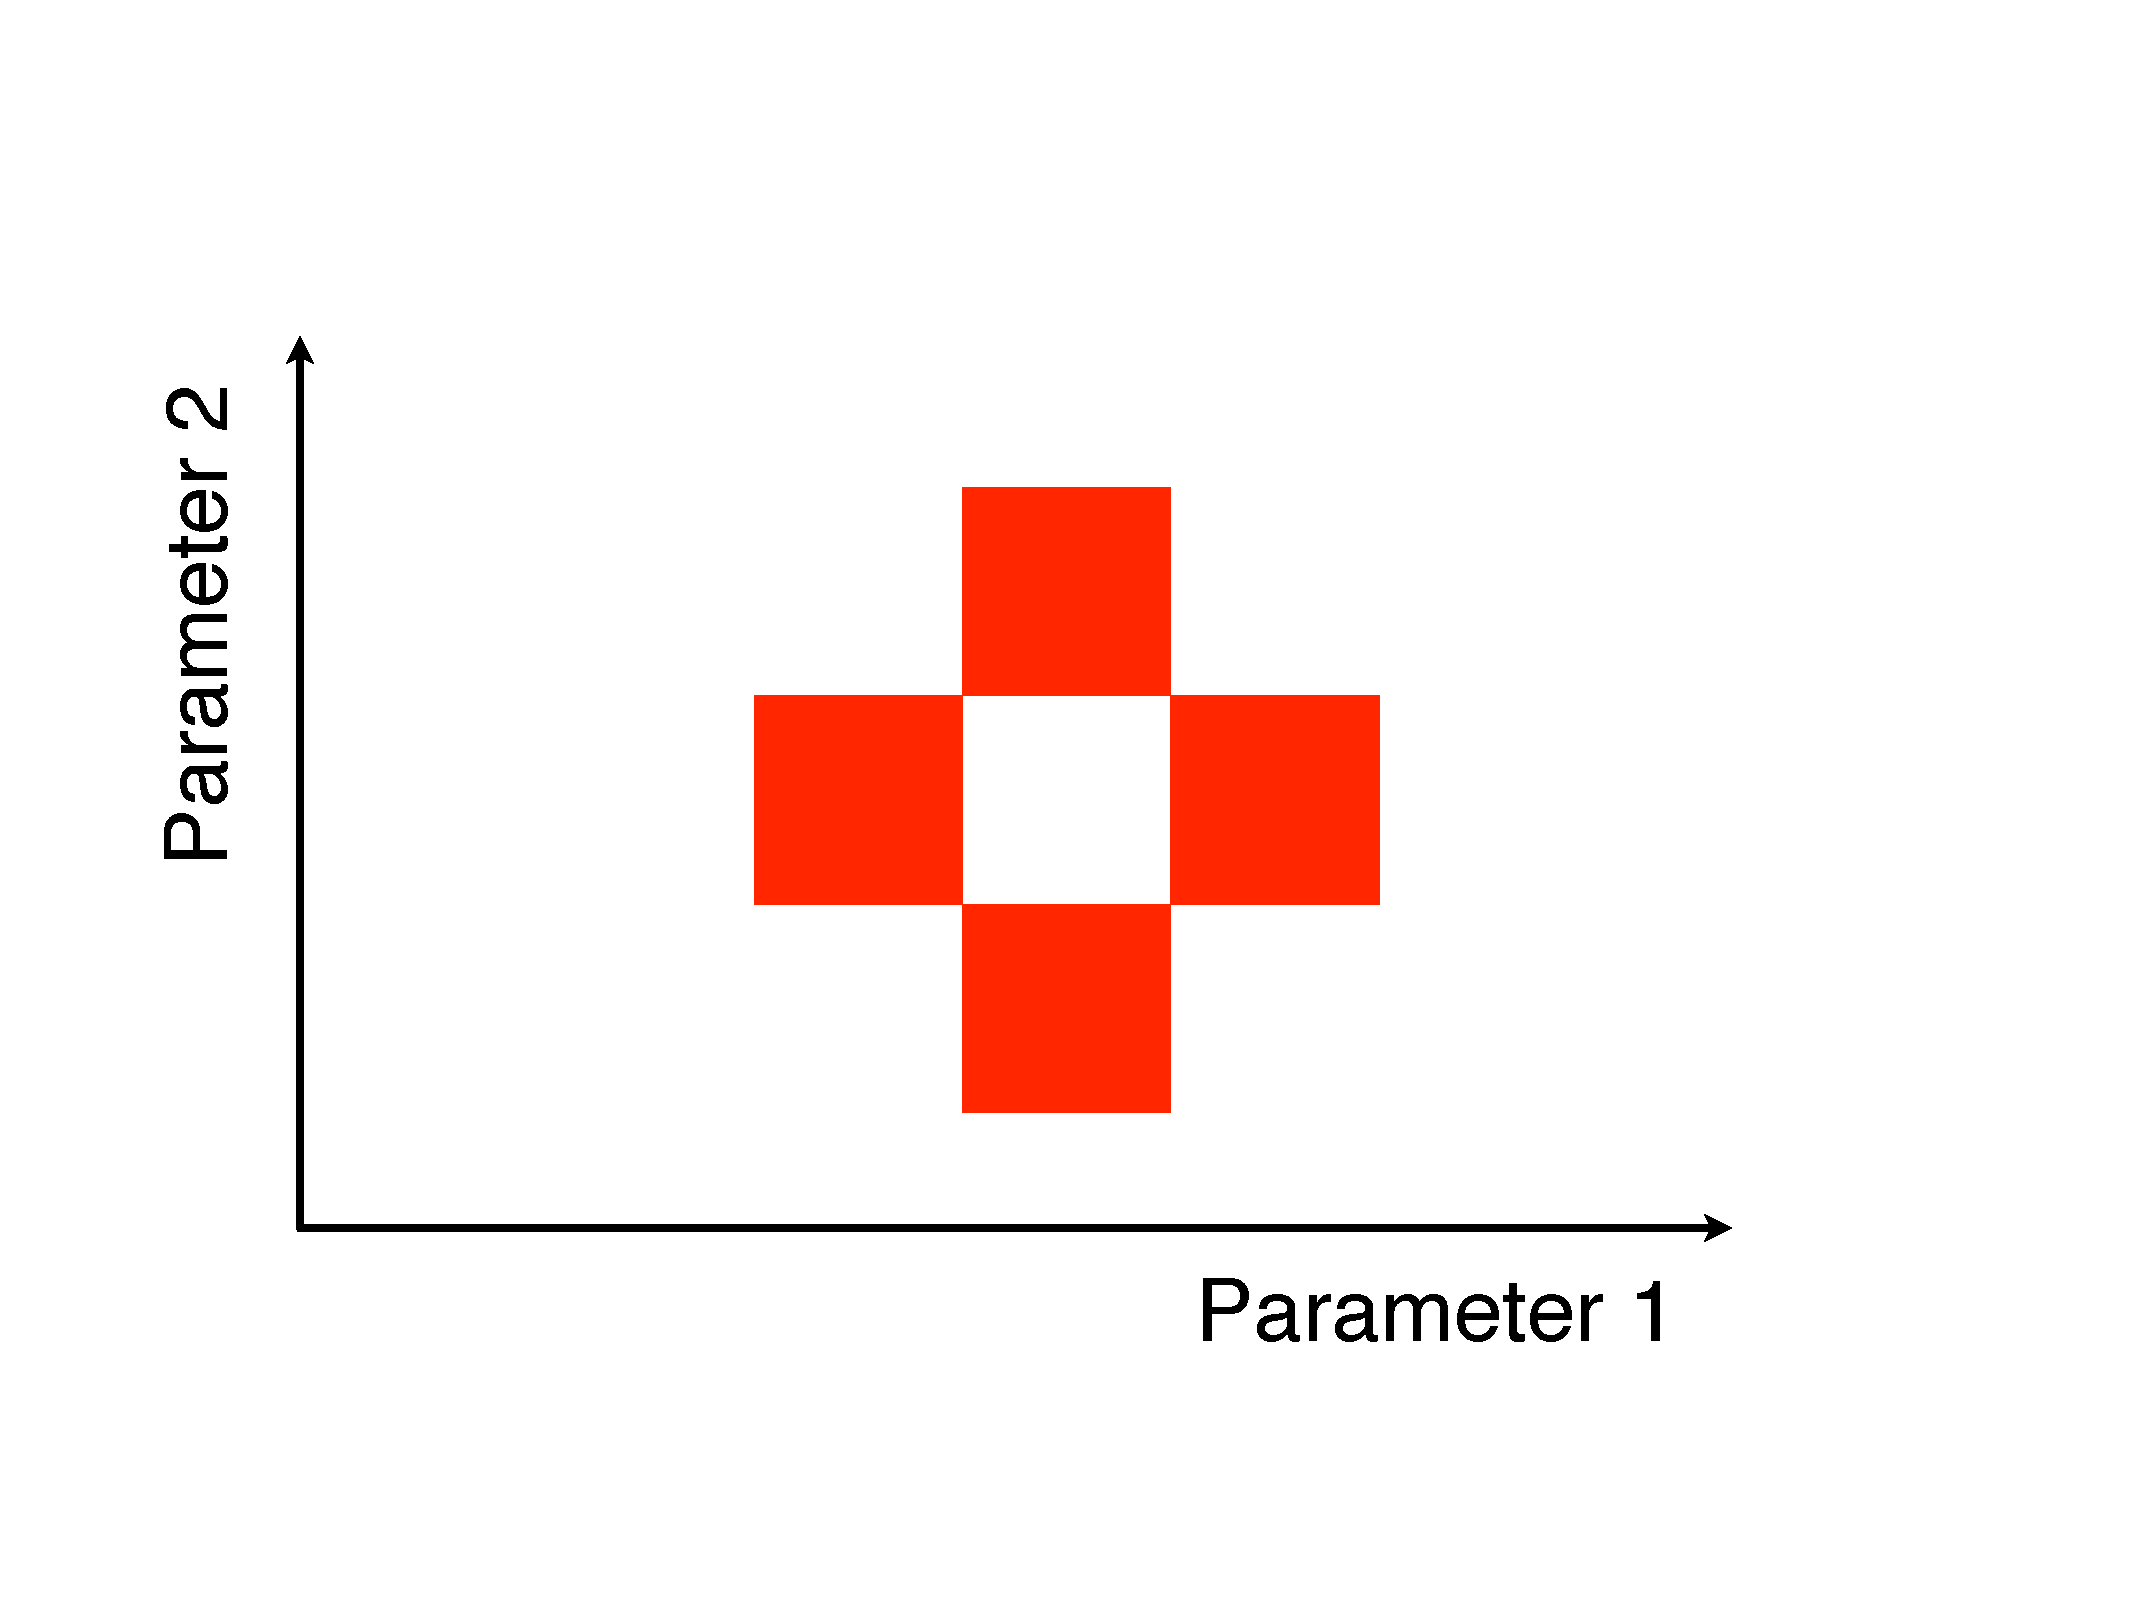
\includegraphics[scale=0.3]{UL_estimation_points}
	\caption{Diagram of the points (red squares) used in the estimation of an upper limit when a computational failure occurs (middle white square).}
	\label{fig:UL_estimation_points}
\end{figure}

\section{Exclusion Contours}
\label{sec:Exclusion Contours}

Exclusion contours for the GMSB models discussed above are shown in Figure~\ref{fig:exclusion_contours}.  The contours are derived from plots of predicted cross section minus cross section upper limit ($\sigma\times(1 - \mu^{95\%\mathrm{CL}})$, where $\sigma$ is the nominal value of the predicted cross section for a given GMSB model) vs. the two model parameters of interest, so the values are either negative (not excluded) or positive (excluded).  Sometimes, a particular point may have a different sign than its four same-sign neighbors (cf. Fig.~\ref{fig:UL_estimation_points}) due to a fluctuation.  In these cases, $\sigma\times(1 - \mu^{95\%\mathrm{CL}})$ for the anomalous point is estimated as the average $\sigma\times(1 - \mu^{95\%\mathrm{CL}})$ of the four neighboring points.  The errors on the individual values of $\sigma\times(1 - \mu^{95\%\mathrm{CL}})$ used in the estimate are propagated to the error on the average.

\begin{figure}
	\centering
	\subfloat[$M_{2}$ decoupled ($M_{2}$ = 3.5 TeV), $M_{1}$ = 375 GeV, $M_{3}$ vs. $m_{\tilde{q}}$, $\geq0$ jets.]{\label{fig:exclusion_contours_mgluino_vs_msquark_bino}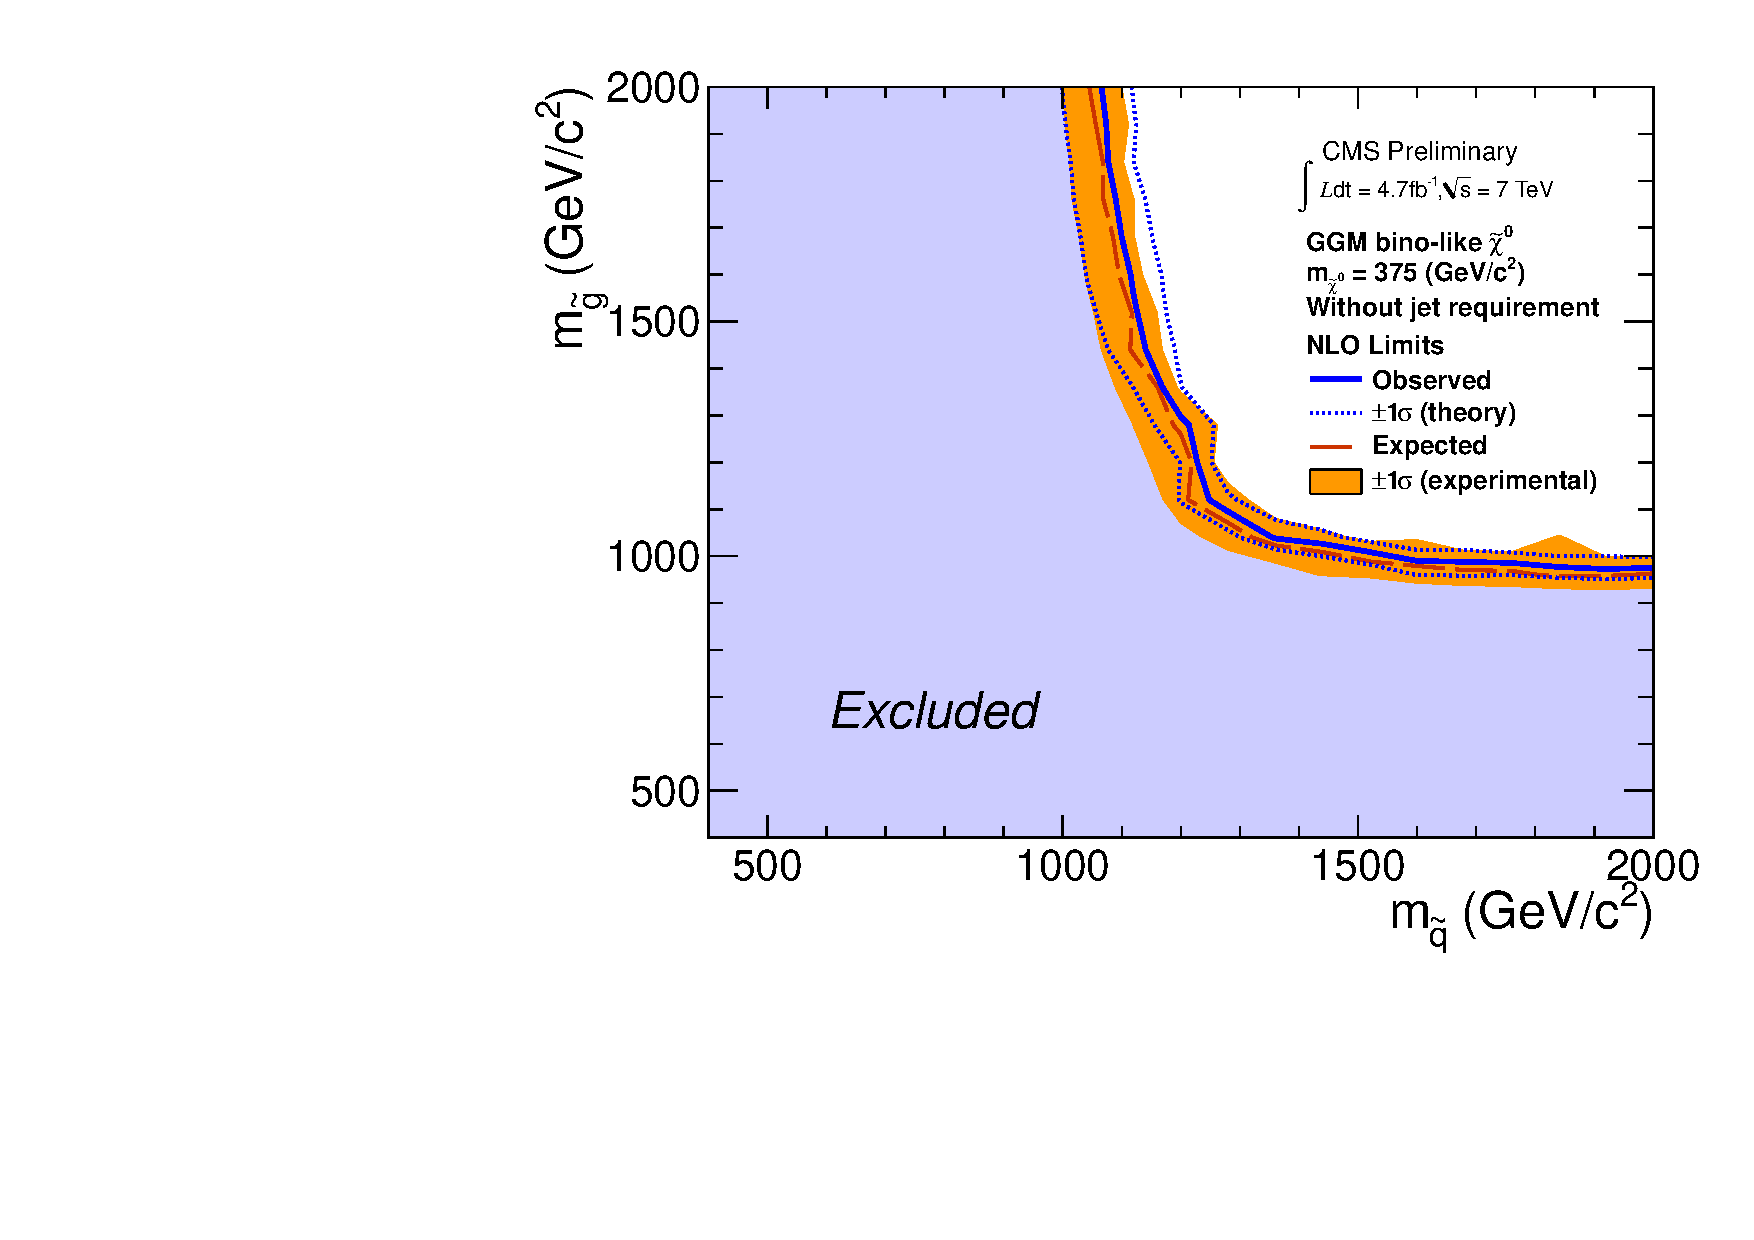
\includegraphics[scale=0.3]{can_excl02_bino_mN375_met100_nojet}}
	\hspace{1cm}
	\subfloat[$M_{2}$ decoupled ($M_{2}$ = 3.5 TeV), $M_{1}$ = 375 GeV, $M_{3}$ vs. $m_{\tilde{q}}$, $\geq1$ jet.]{\label{fig:exclusion_contours_mgluino_vs_msquark_bino_1jet}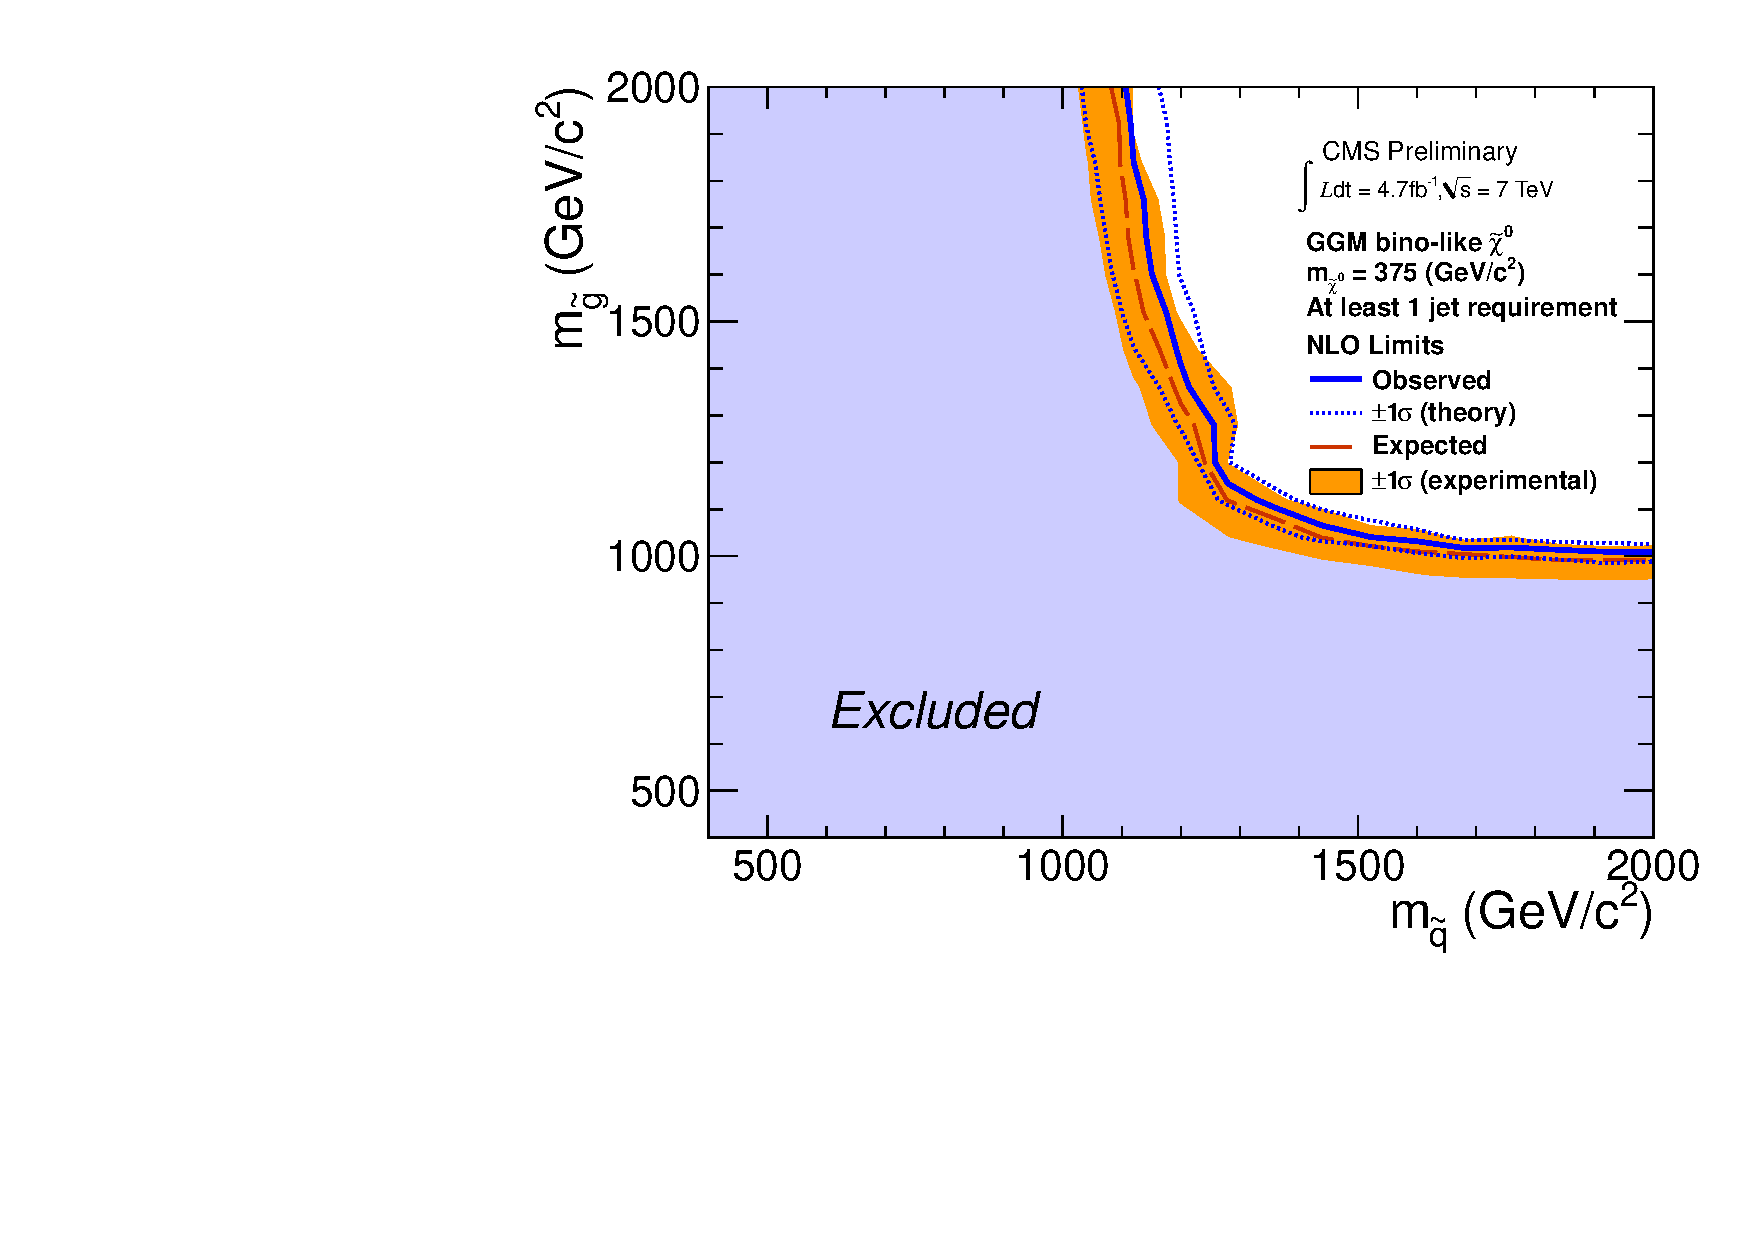
\includegraphics[scale=0.3]{can_excl02_bino_mN375_met100_1jet}}
	\\
	\subfloat[$M_{1}$ decoupled ($M_{1}$ = 3.5 TeV), $M_{2}$ = 375 GeV, $M_{3}$ vs. $m_{\tilde{q}}$, $\geq0$ jets.]{\label{fig:exclusion_contours_mgluino_vs_msquark_wino}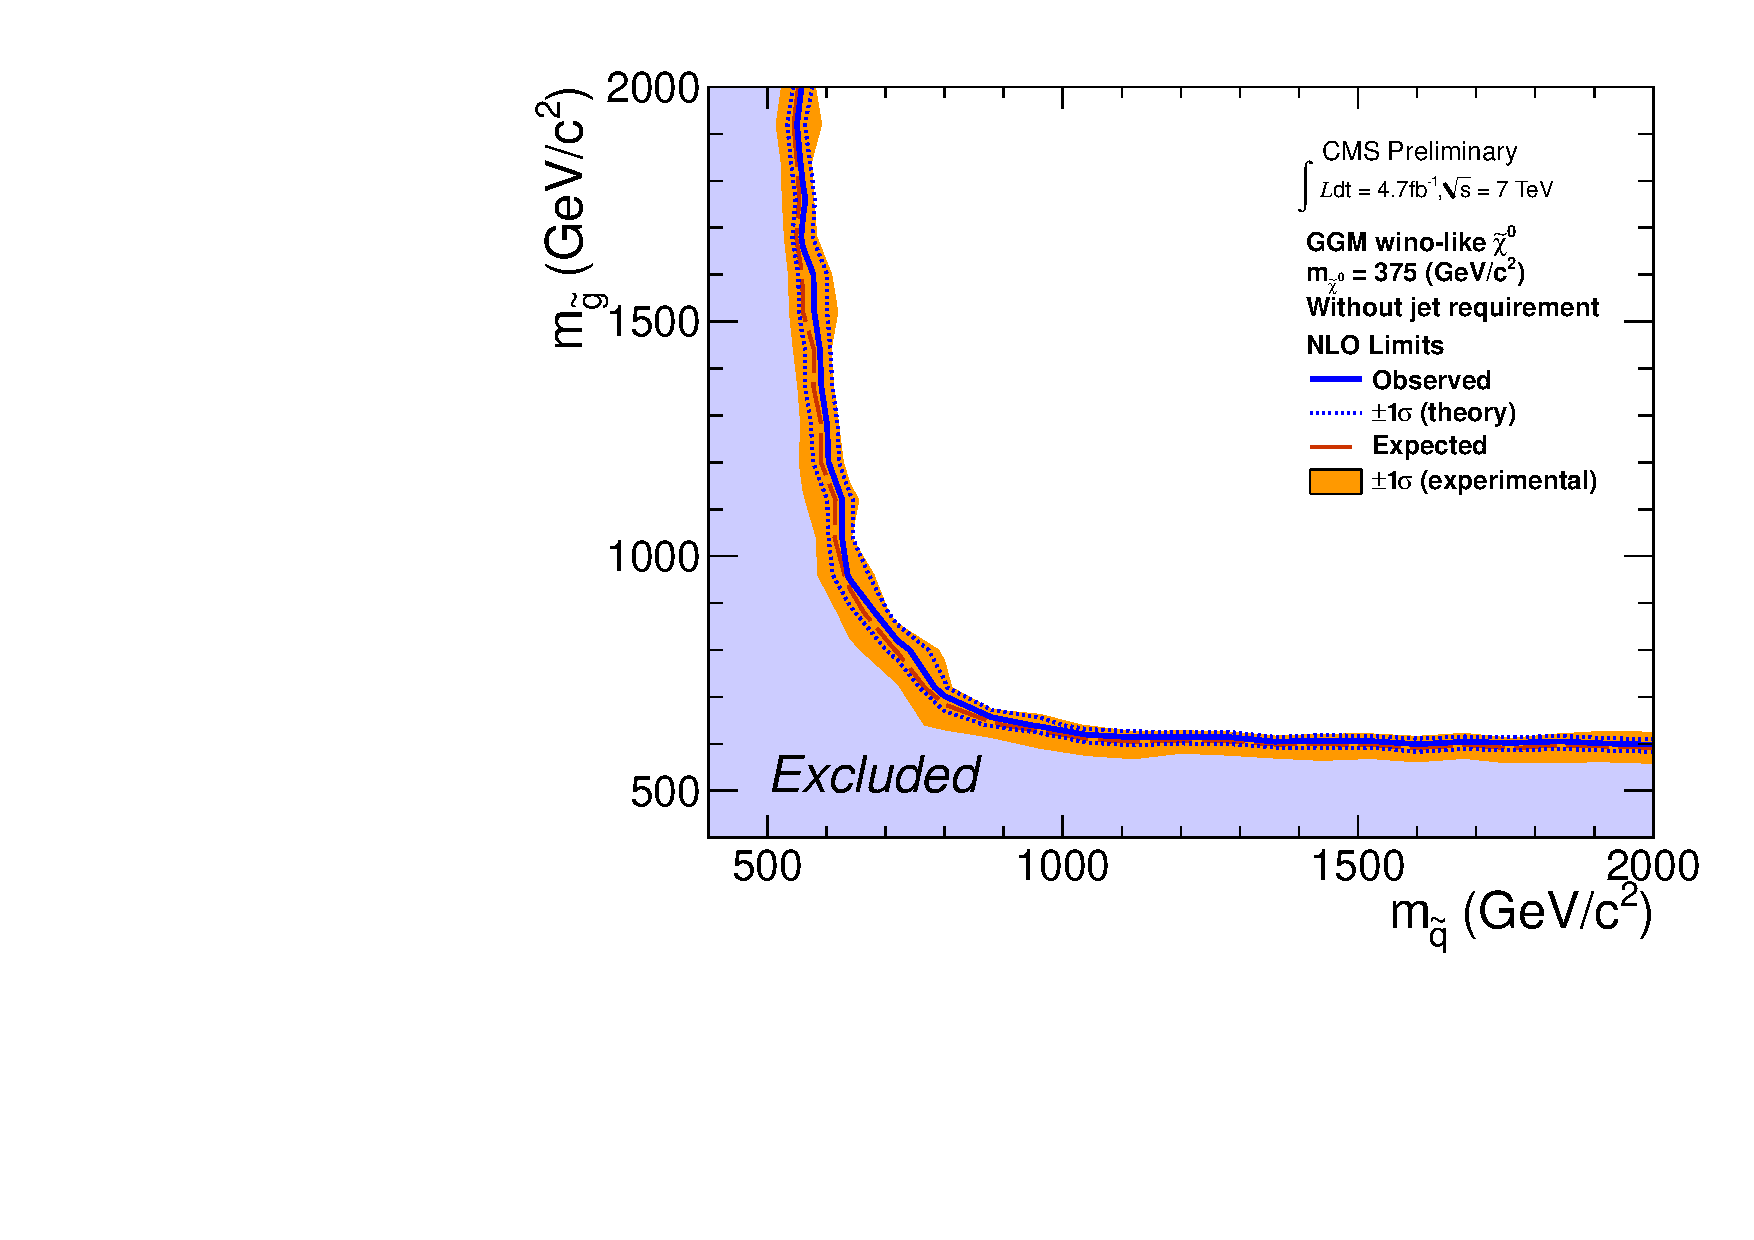
\includegraphics[scale=0.3]{can_excl02_wino_mN375_met100_nojet}}
	\hspace{1cm}
	\subfloat[$M_{1}$ decoupled ($M_{1}$ = 3.5 TeV), $M_{2}$ = 375 GeV, $M_{3}$ vs. $m_{\tilde{q}}$, $\geq1$ jet.]{\label{fig:exclusion_contours_mgluino_vs_msquark_wino_1jet}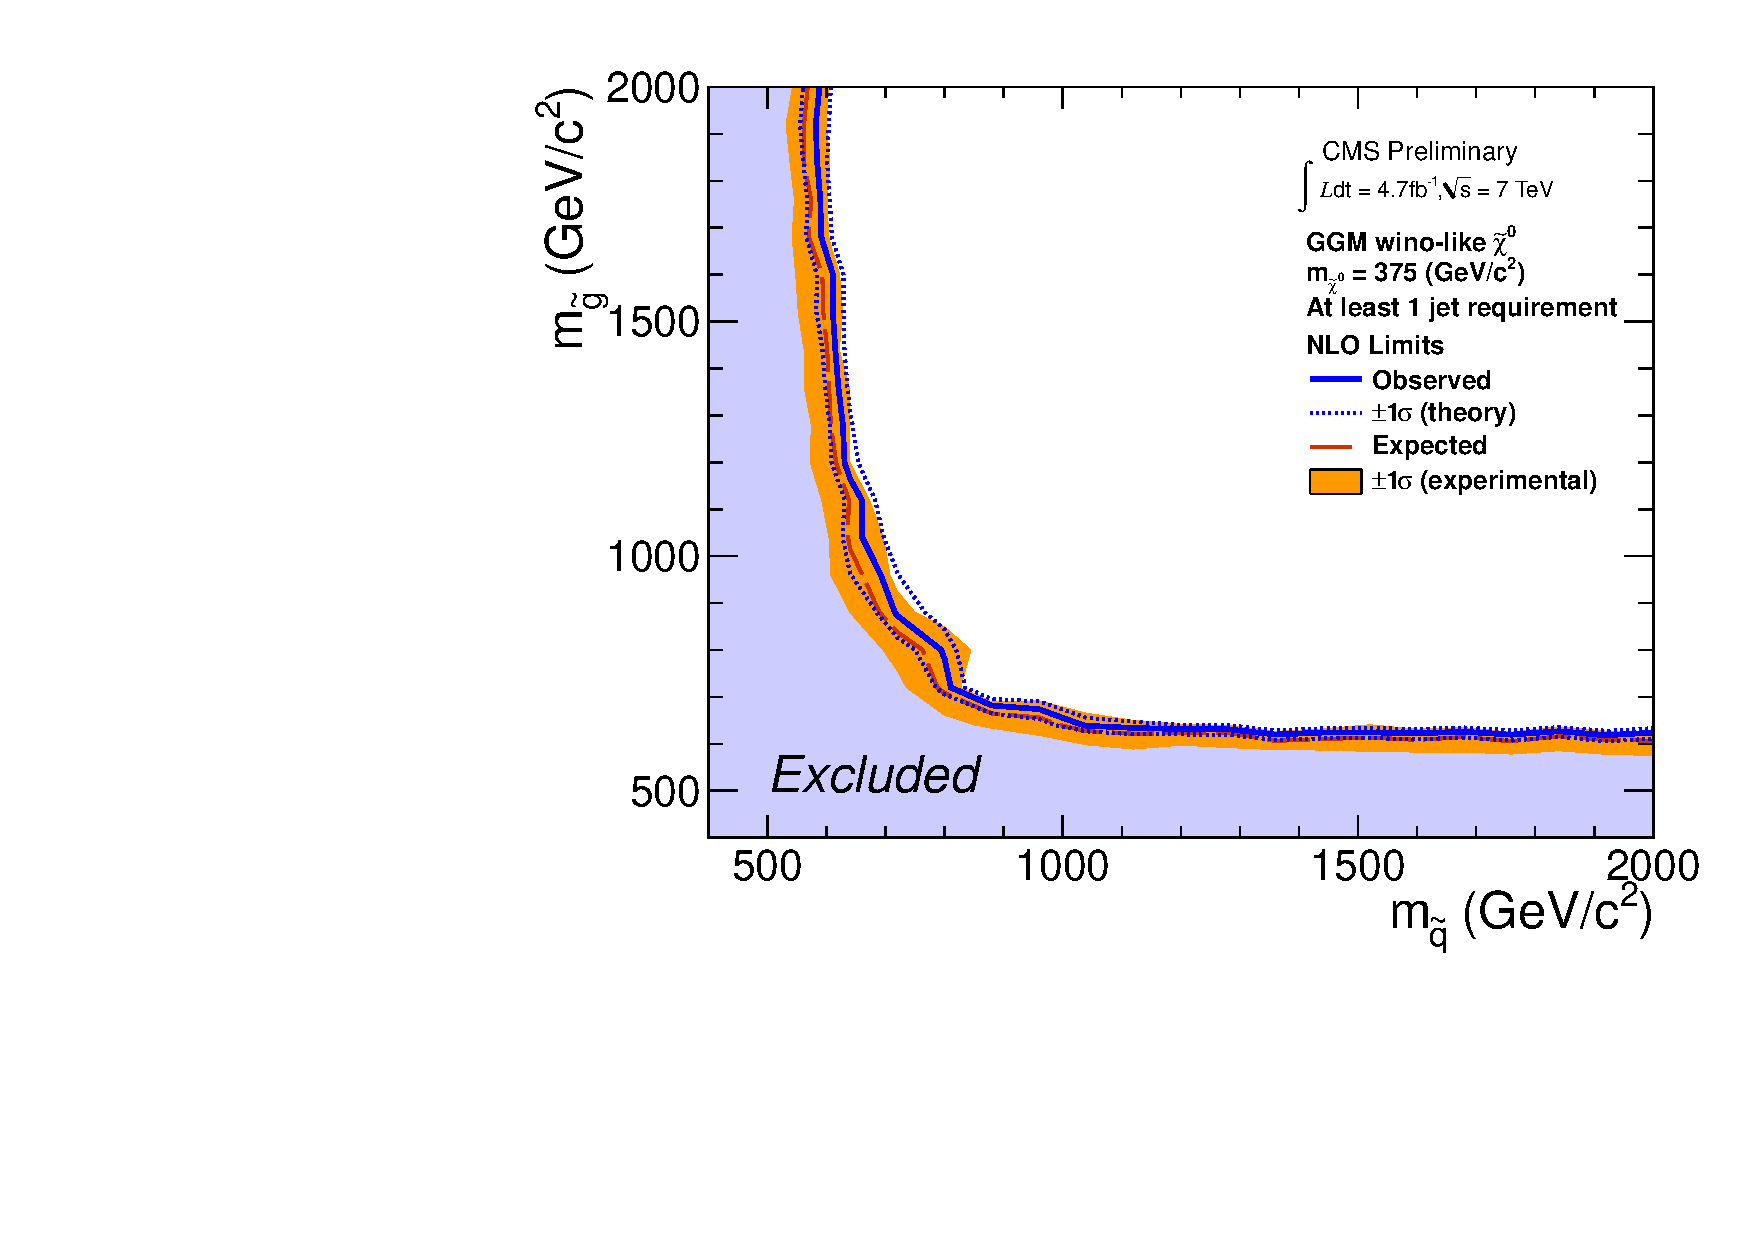
\includegraphics[scale=0.3]{can_excl02_wino_mN375_met100_1jet}}
	\\
	\subfloat[$m_{\tilde{q}}$ decoupled ($m_{\tilde{q}}$ = 2.5 TeV), $M_{3}$ vs. $M_{1}$, $\geq0$ jets.]{\label{fig:exclusion_contours_mgluino_vs_mbino_old}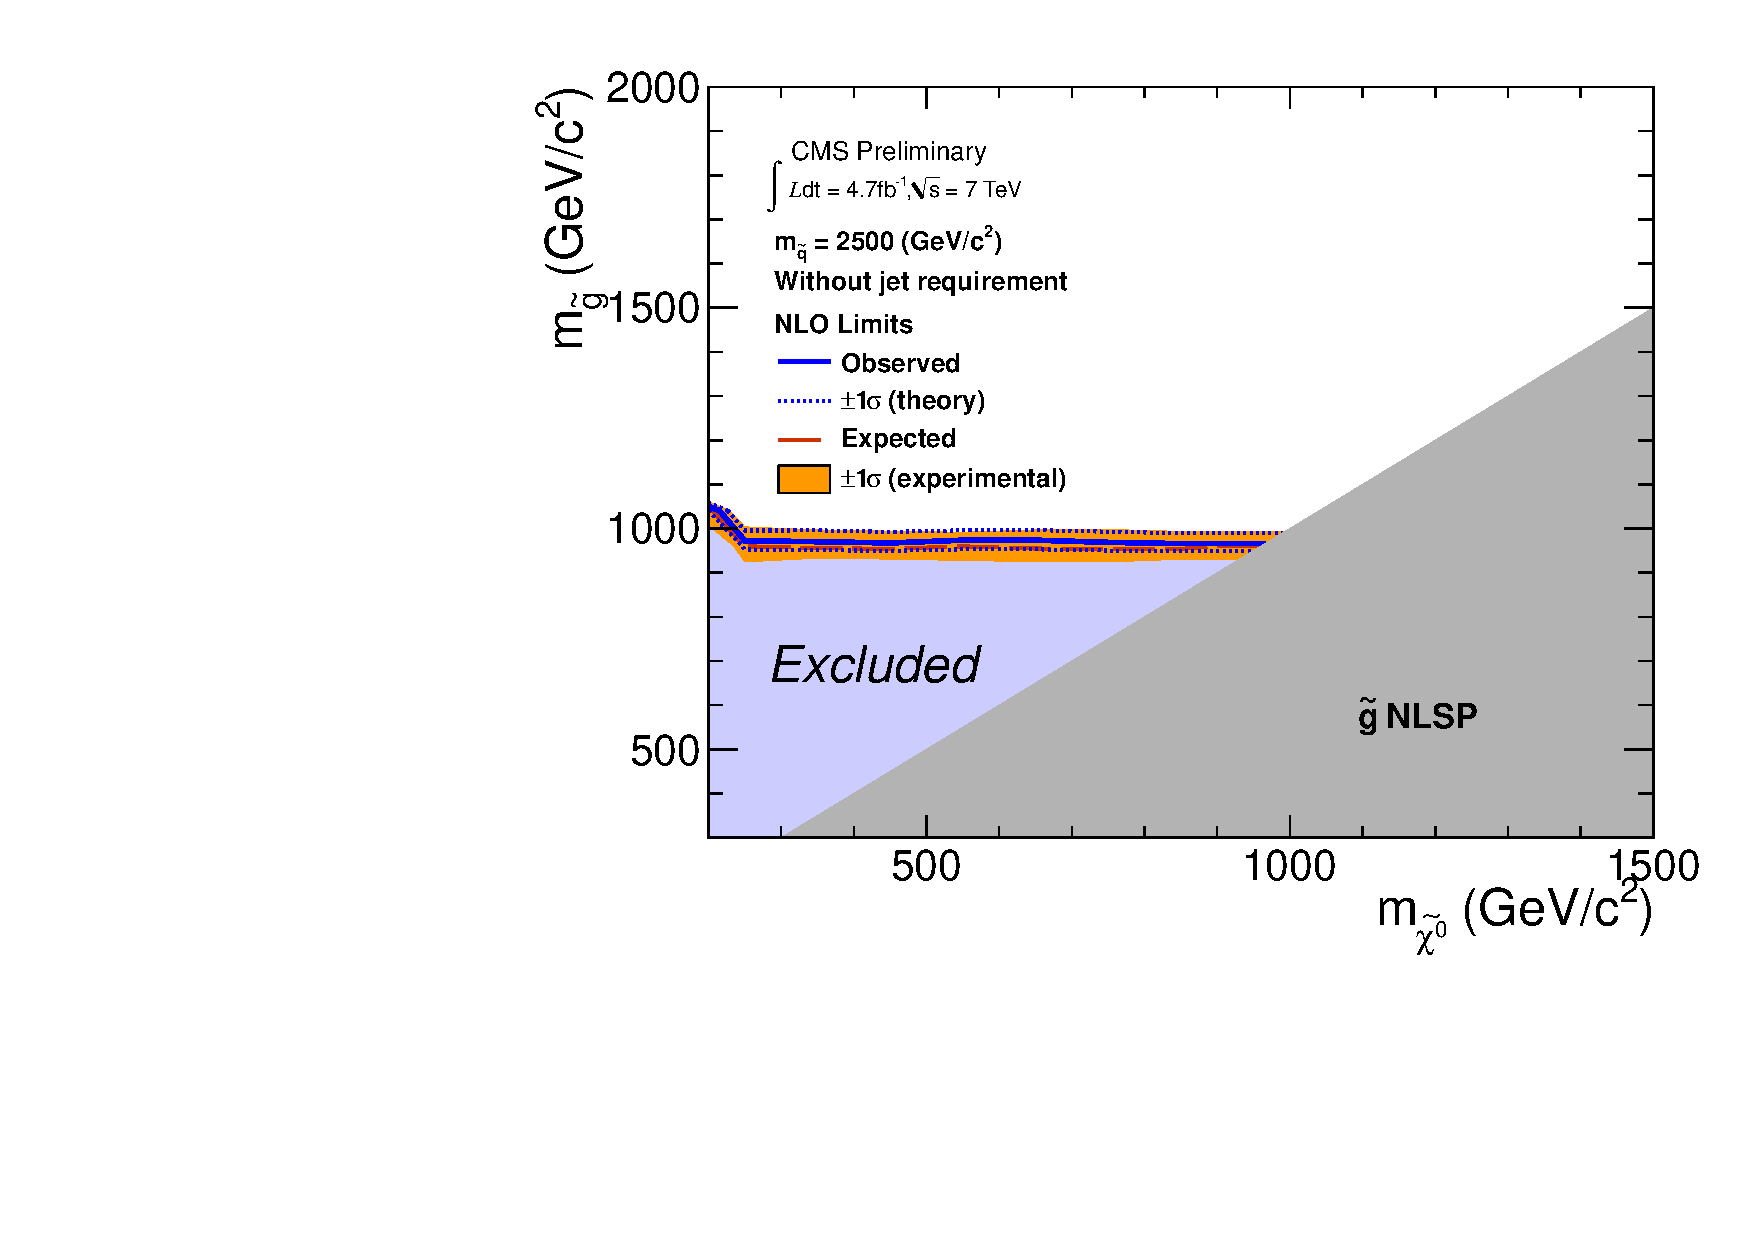
\includegraphics[scale=0.3]{can_excl02_bino_mNScan_met100_nojet}}
	\hspace{1cm}
	\subfloat[$m_{\tilde{q}}$ decoupled ($m_{\tilde{q}}$ = 2.5 TeV), $M_{3}$ vs. $M_{1}$, $\geq1$ jet.]{\label{fig:exclusion_contours_mgluino_vs_mbino_old_1jet}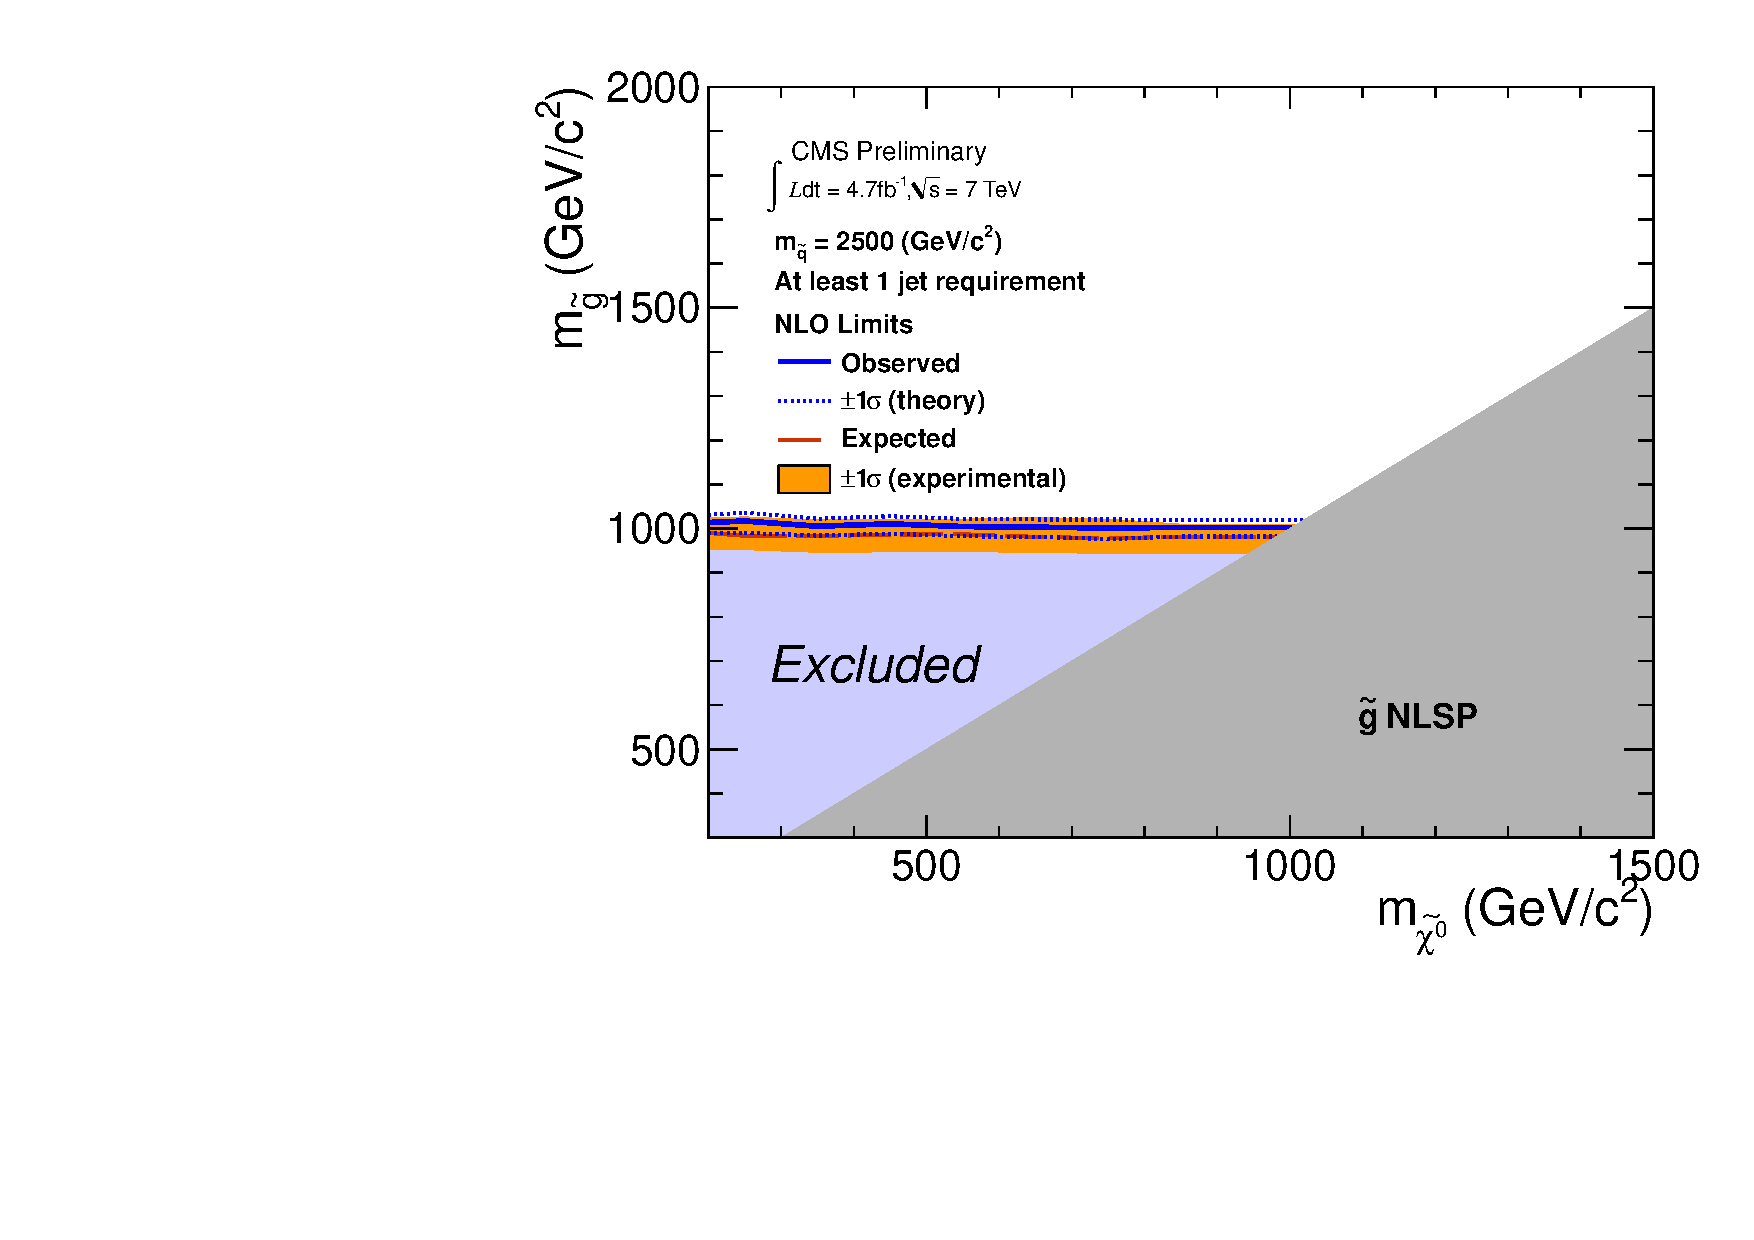
\includegraphics[scale=0.3]{can_excl02_bino_mNScan_met100_1jet}}
	\caption{Exclusion contours for the three different scenarios described in Sec.~\ref{sec:Simplified Models}.}
	\label{fig:exclusion_contours}
\end{figure}

In the plots in Fig.~\ref{fig:exclusion_contours}, the expected limit (i.e. the contour derived from $\sigma\times(1 - \mu_{\mathrm{exp,scan}}^{95\%\mathrm{CL}})$) is drawn in dark orange and the $1\sigma$ experimental band around the expected limit (i.e. the shaded region between the contours derived from $\sigma\times(1 - \mu^{95\%\mathrm{CL}}_{\pm1\sigma\mathrm{,scan}})$) is drawn in light orange.  The values of $\mu_{\mathrm{exp,scan}}^{95\%\mathrm{CL}}$ and $\mu^{95\%\mathrm{CL}}_{\pm1\sigma\mathrm{,scan}}$ only reflect the experimental uncertainties given in Sec.~\ref{sec:Profile Likelihood}.

The observed limits (derived from $\sigma\times(1 - \mu_{\mathrm{obs,scan}}^{95\%\mathrm{CL}})$) and $1\sigma$ theoretical error bands around the observed limits in Fig.~\ref{fig:exclusion_contours} are drawn in blue.  The contours that define this band are derived from $\pm(\sigma_{\pm1\sigma} - \sigma\mu_{\mathrm{obs,scan}}^{95\%\mathrm{CL}})$, where $\sigma_{\pm1\sigma}$ is the nominal value of the predicted cross section $\pm$ the one-standard-deviation theoretical error on the predicted cross section.  In this way, the experimental and theoretical errors, the latter due to imperfect knowledge of the predicted cross section, are shown separately.  Comparing with Fig.~\ref{fig:sig_xsec}, one can easily see that the shapes of the exclusion curves are driven by the contours in the expected cross section plane.  In all the plots, the observed limit is slightly higher than the expected limit, reflecting the fact that the background prediction is slightly higher than the observation.

The dominant theoretical uncertainties on the GMSB cross sections are due to:

\begin{itemize}
\item PDF uncertainty (4\%-100\% depending on model)
\item Renormalization scale uncertainty (0.036\%-25\% depending on model)
\end{itemize}
%
The PDF4LHC \cite{PDF4LHC} recommendations are used to calculate the effect of these uncertainties on the GMSB cross sections.  The recommendations state that PDF sets from MSTW08 \cite{MSTW08}, CTEQ6.6 \cite{CTEQ6}, and NNPDF2.0 \cite{NNPDF2_0} should be considered in the determination of the PDF uncertainties, because these three PDF sets include constraints from the Tevatron and from fixed target experiments, as well as from HERA \cite{HERA}, and are thus the most complete.

Each collaboration's PDF prediction comes from a global fit to experimental data with a certain number of free parameters.  The best fit parameters come from minimizing the $\chi^{2}$; increasing the $\chi^{2}$ by one from its minimum can be written in terms of the $N$-dimensional Hessian error matrix \cite{Hessian} where $N$ is the number of free parameters.  To form the $i^{\mathrm{th}}$ pair of members of the PDF set, the PDF is evaluated once at the parameter values given by the $i^{\mathrm{th}}$ eigenvector of the Hessian matrix, and then again at the parameter values given by the negative of the $i^{\mathrm{th}}$ eigenvector.  Each PDF set therefore contains 2$N$ members, corresponding to the positive and negative values of the $N$ eigenvectors \cite{PDF_primer}.

To calculate the PDF uncertainties for a given GMSB model, the leading order Pythia cross section is reweighted by a factor of the error PDF divided by the leading order PDF with which the model was generated.  This is repeated for each error PDF in a given PDF set.  The $\pm1\sigma$ deviations are proportional to the maximum difference between cross sections obtained this way.  The actual equation for the $\pm1\sigma$ errors is Eq. (43) of ref. \cite{PDF_primer}.  In the same way, the $\pm1\sigma$ errors are calculated for the CTEQ6.6, MSTW08, and NNPDF2.0 PDF sets.  
The total error is given by the half the difference between the largest $+1\sigma$ deviation and the smallest $-1\sigma$ deviation \cite{PDF4LHC}.

The uncertainties on the signal cross sections due to the choice of renormalization/factorization scale ($\alpha_{S}(M_{Z})$) are evaluated by calculating the PROSPINO next to leading order cross section once with $\alpha_{S}(M_{Z})$ halved, then once with $\alpha_{S}(M_{Z})$ doubled.  The lower error on the cross section is taken as the absolute difference between the nominal and halved-scale values of the cross section, while the upper error is taken as the absolute difference between the nominal and doubled-scale values.  The PDF and $\alpha_{S}$ uncertainties are added in quadrature to give the total PDF uncertainty.

Note that the quoted GMSB cross sections are evaluated at next to leading order using PROSPINO, but it is the leading order Pythia cross sections that are reweighted to the next to leading order MSTW08, CTEQ6.6, and NNPDF2.0 PDFs to get the error bands.  In addition, since to a good approximation the GMSB production cross sections for the $M_{3}$-$m_{\tilde{q}}$ scans only depend on $M_{3}$ and $m_{\tilde{q}}$, the same PDF errors per point are used for the $\tilde{B}$-like and $\tilde{W}$-like grids.

\end{document}